\documentclass[12pt,oneside,letterpaper,francais]{book}

%% \documentclass[12pt]{report}

\usepackage[french, english]{babel}
%\usepackage{isolatin1}
\usepackage[utf8]{inputenc}
\usepackage{url}
\usepackage{setspace}
\usepackage{verbatim}

\usepackage{udem_these_fr}

\newcommand{\todo}[1]{[TODO: {\it #1}]}

%\newcommand{\object}[1]{$\#<#1 \ldots>$}
\newcommand{\object}[1]{{\it #1}}

\newcommand{\ie}{{\textit{i.e.}}}

% Macros for R^nRS.

\makeatletter

\newcommand{\topnewpage}{\@topnewpage}
\newcommand{\authorsc}[1]{{\scriptsize\scshape #1}}

% Chapters, sections, etc.

\newcommand{\extrapart}[1]{
 % \chapter{#1}
  \chapter*{#1}
  \markboth{#1}{#1}
  \vskip 1ex
  \addcontentsline{toc}{chapter}{#1}}

\newcommand{\clearchapterstar}[1]{
  \clearpage
  \topnewpage[
    \centerline{\large\bf\uppercase{#1}}
    \bigskip]}

\newcommand{\clearextrapart}[1]{
  \clearchapterstar{#1}
  \markboth{#1}{#1}
  \addcontentsline{toc}{chapter}{#1}}

\newcommand{\vest}{}
\newcommand{\dotsfoo}{$\ldots\,$}

\newcommand{\sharpfoo}[1]{{\tt\##1}}
\newcommand{\schfalse}{\sharpfoo{f}}
\newcommand{\schtrue}{\sharpfoo{t}}

\newcommand{\singlequote}{{\tt'}}  %\char19
\newcommand{\doublequote}{{\tt"}}
\newcommand{\backquote}{{\tt\char18}}
\newcommand{\backwhack}{{\tt\char`\\}}
\newcommand{\atsign}{{\tt\char`\@}}
\newcommand{\sharpsign}{{\tt\#}}
\newcommand{\verticalbar}{{\tt|}}

\newcommand{\coerce}{\discretionary{->}{}{->}}

% Knuth's \in sucks big boulders
\def\elem{\hbox{\raise.13ex\hbox{$\scriptstyle\in$}}}

\newcommand{\meta}[1]{{\noindent\hbox{\rm$\langle$#1$\rangle$}}}
\let\hyper=\meta
\newcommand{\hyperi}[1]{\hyper{#1$_1$}}
\newcommand{\hyperii}[1]{\hyper{#1$_2$}}
\newcommand{\hyperj}[1]{\hyper{#1$_i$}}
\newcommand{\hypern}[1]{\hyper{#1$_n$}}
\newcommand{\var}[1]{\noindent\hbox{\it{}#1\/}}  % Careful, is \/ always the right thing?
\newcommand{\vari}[1]{\var{#1$_1$}}
\newcommand{\varii}[1]{\var{#1$_2$}}
\newcommand{\variii}[1]{\var{#1$_3$}}
\newcommand{\variv}[1]{\var{#1$_4$}}
\newcommand{\varj}[1]{\var{#1$_j$}}
\newcommand{\varn}[1]{\var{#1$_n$}}

\newcommand{\vr}[1]{{\noindent\hbox{$#1$\/}}}  % Careful, is \/ always the right thing?
\newcommand{\vri}[1]{\vr{#1_1}}
\newcommand{\vrii}[1]{\vr{#1_2}}
\newcommand{\vriii}[1]{\vr{#1_3}}
\newcommand{\vriv}[1]{\vr{#1_4}}
\newcommand{\vrv}[1]{\vr{#1_5}}
\newcommand{\vrj}[1]{\vr{#1_j}}
\newcommand{\vrn}[1]{\vr{#1_n}}


\newcommand{\defining}[1]{\mainindex{#1}{\em #1}}
\newcommand{\ide}[1]{{\schindex{#1}\frenchspacing\tt{#1}}}

\newcommand{\lambdaexp}{{\cf lambda} expression}
\newcommand{\Lambdaexp}{{\cf Lambda} expression}

\newcommand{\callcc}{{\tt call-with-current-continuation}}

% \reallyindex{SORTKEY}{HEADCS}{TYPE}
% writes (index-entry "SORTKEY" "HEADCS" TYPE PAGENUMBER)
% which becomes  \item \HEADCS{SORTKEY} mainpagenumber ; auxpagenumber ...

\global\def\reallyindex#1#2#3{%
\write\@indexfile{"#1" "#2" #3 \thepage}}

\newcommand{\mainschindex}[1]{\label{#1}\reallyindex{#1}{tt}{main}}
\newcommand{\mainindex}[1]{\reallyindex{#1}{rm}{main}}
\newcommand{\schindex}[1]{\reallyindex{#1}{tt}{aux}}
\newcommand{\sharpindex}[1]{\reallyindex{#1}{sharpfoo}{aux}}
\renewcommand{\index}[1]{\reallyindex{#1}{rm}{aux}}

\newcommand{\domain}[1]{#1}
\newcommand{\nodomain}[1]{}
%\newcommand{\todo}[1]{{\rm$[\![$!!~#1$]\!]$}}
%\newcommand{\todo}[1]{}

% \frobq will make quote and backquote look nicer.
\def\frobqcats{%\catcode`\'=13
\catcode`\`=13{}}
{\frobqcats
\gdef\frobqdefs{%\def'{\singlequote}
\def`{\backquote}}}
\def\frobq{\frobqcats\frobqdefs}

% \cf = code font
% Unfortunately, \cf \cf won't work at all, so don't even attempt to
% next constructions which use them...
\newcommand{\cf}{\frobq\tt}

% Same as \obeycr, but doesn't do a \@gobblecr.
{\catcode`\^^M=13 \gdef\myobeycr{\catcode`\^^M=13 \def^^M{\\}}%
\gdef\restorecr{\catcode`\^^M=5 }}

{\catcode`\^^I=13 \gdef\obeytabs{\catcode`\^^I=13 \def^^I{\hbox{\hskip 4em}}}}

{\obeyspaces\gdef {\hbox{\hskip0.5em}}}

\gdef\gobblecr{\@gobblecr}

\def\setupcode{\@makeother\^}

% Scheme example environment
% At 11 points, one column, these are about 56 characters wide.
% That's 32 characters to the left of the => and about 20 to the right.

\newenvironment{schemecode}{
  % Commands for scheme examples
  \newcommand{\ev}{\>\>\>\evalsto}
  \newcommand{\lev}{\\\>\evalsto}
  \newcommand{\unspecified}{{\em{}unspecified}}
  \newcommand{\scherror}{{\em{}error}}
  \setupcode
  \cf \obeytabs \obeyspaces \myobeycr
  \vspace{-1.5em}
  \selectlanguage{english}
  \begin{singlespace}
  %\begin{minipage}
  \begin{tabbing}%
\qquad\=\hspace*{5em}\=\hspace*{9em}\=\kill%   was 16em
\gobblecr}{\unskip
\end{tabbing}
%\end{minipage}
\end{singlespace}
\selectlanguage{french}
\vspace{-1.5em}
}

%\newenvironment{scheme}{\begin{schemenoindent}\+\kill}{\end{schemenoindent}}
\newenvironment{schemewithindent}{
  % Commands for scheme examples
  \newcommand{\ev}{\>\>\evalsto}
  \newcommand{\lev}{\\\>\evalsto}
  \renewcommand{\em}{\rmfamily\itshape}
  \newcommand{\unspecified}{{\em{}unspecified}}
  \newcommand{\scherror}{{\em{}error}}
  \setupcode
  \cf \obeyspaces \myobeycr
  \begin{tabbing}%
\qquad\=\hspace*{5em}\=\hspace*{9em}\=\+\kill%   was 16em
\gobblecr}{\unskip\end{tabbing}}

\newcommand{\evalsto}{$\Longrightarrow$}

% Rationale

\newenvironment{rationale}{%
\bgroup\small\noindent{\em Rationale:}\space}{%
\egroup}

% Notes

\newenvironment{note}{%
\bgroup\small\noindent{\em Note:}\space}{%
\egroup}

% Manual entries

\newenvironment{entry}[1]{
  \vspace{3.1ex plus .5ex minus .3ex}\noindent#1%
\unpenalty\nopagebreak}{\vspace{0ex plus 1ex minus 1ex}}

\newcommand{\exprtype}{syntax}

% Primitive prototype
\newcommand{\pproto}[2]{\unskip%
\hbox{\cf\spaceskip=0.5em#1}\hfill\penalty 0%
\hbox{ }\nobreak\hfill\hbox{\rm #2}\break}

% Parenthesized prototype
\newcommand{\proto}[3]{\pproto{(\mainschindex{#1}\hbox{#1}{\it#2\/})}{#3}}

% Variable prototype
\newcommand{\vproto}[2]{\mainschindex{#1}\pproto{#1}{#2}}

% Extending an existing definition (\proto without the index entry)
\newcommand{\rproto}[3]{\pproto{(\hbox{#1}{\it#2\/})}{#3}}

% Grammar environment

\newenvironment{grammar}{
  \def\:{\goesto{}}
  \def\|{$\vert$}
  \cf \myobeycr
  \begin{tabbing}
    %\qquad\quad \= 
    \qquad \= $\vert$ \= \kill
  }{\unskip\end{tabbing}}

%\newcommand{\unsection}{\unskip}
\newcommand{\unsection}{{\vskip -2ex}}

% Commands for grammars
\newcommand{\arbno}[1]{#1\hbox{\rm*}}  
\newcommand{\atleastone}[1]{#1\hbox{$^+$}}

\newcommand{\goesto}{$\longrightarrow$}

% The index

\def\theindex{%\@restonecoltrue\if@twocolumn\@restonecolfalse\fi
%\columnseprule \z@
%!! \columnsep 35pt
\clearpage
\@topnewpage[
    \centerline{\large\bf\uppercase{Alphabetic index of definitions of concepts,}}
    \centerline{\large\bf\uppercase{keywords, and procedures}}
    \vskip 1ex \bigskip]
    \markboth{Index}{Index}
    \addcontentsline{toc}{chapter}{Alphabetic index of 
 definitions of concepts,\hfil\penalty0 \hbox{\hspace*{2em} keywords, and procedures}}
    \bgroup %\small
    \parindent\z@
    \parskip\z@ plus .1pt\relax\let\item\@idxitem}

\def\@idxitem{\par\hangindent 40pt}

\def\subitem{\par\hangindent 40pt \hspace*{20pt}}

\def\subsubitem{\par\hangindent 40pt \hspace*{30pt}}

\def\endtheindex{%\if@restonecol\onecolumn\else\clearpage\fi
\egroup}

\def\indexspace{\par \vskip 10pt plus 5pt minus 3pt\relax}

\makeatother


\newcommand{\codeinput}[1]{\begin{singlespace}\verbatiminput{#1}\end{singlespace}}
\newcommand{\schemeinput}[1]{\begin{schemecode}\input{#1}\end{schemecode}}

\newcommand{\scheme}[1]{\selectlanguage{english}{\tt #1}\selectlanguage{french}}
\newcommand{\schemeresult}[1]{{\it #1}}

%% \hyphenation{ex-écu-tion} %% marche pas a cause de l'accent

\title{Développement de jeux vidéo en Scheme}

% remplir les champs...
\Auteur{David}{St-Hilaire}

\President{M.}{Mostapha}{Aboulhamid}{Ph.D.}

\Directeur{M.}{Marc}{Feeley}{Ph.D.}

\Membres{1}{M.}{Yann-Gaël}{Guéhéneuc}{Ph.D.}

%pour le doctorat seulement

%examinateur externe
%\Membres{2}{M.}{Membre}{deux}{Ph.D.}
%
%%representant du doyen de la FES
%\Membres{3}{M.}{Membre}{trois}{Ph.D.}

%Pour un doctorat, changer simplement \MSc par \PhD
%titre: 15 mots, max. 175 caractère
\MSc{Dévelopment de jeux vidéo en Scheme}
    {}
    {d'informatique et de recherche op\'{e}rationnelle}
    {informatique}
    {Décembre}
    {2009}

\setstretch{2}
\begin{document}

\setcounter{page}{1}
 \PagesCouverture

\resume


\vspace{2em}

\noindent {\bf Mots clés}: Language de programmation fonctionnels,
Scheme, jeux vidéo, programmation orientée objet.

\abstract

\selectlanguage{english}


\vspace{2em}

\noindent {\bf Keywords}: Functional programming languages, Scheme,
video games, object oriented programming.


\selectlanguage{french}

%% \maketitle
 
\tabledesmatieres

% \listedestableaux

\listedesfigures

% \listedesannexes

\remerciements

blablabla

% \preface
% 
% Préface...

\debutchapitres

%%%%%%%%%%%%%%%%%%%%%%%%%%%%%%%%%%%%%%%%%%%%%%%%%%%%%%%%%%%%%%%%%%%%%%%%%%%%%%%
\chapter{Introduction}
\label{Chap:Intro}

L'industrie du jeu vidéo devient de plus en plus importante dans le
domaine de l'informatique. Cette croissance est bien reflétée par
l'augmentation de 28\% des revenus provenant de la vente de jeux vidéo
aux États-Unis durant l'année 2007~\cite{NPD_Games_2007}. La place
occupée par l'industrie du jeu vidéo durant cette même année s'estime
à 76\% du marché de tous les logiciels vendus~\cite{NPD_Soft_2008}. 

L'engouement du marché du jeu vidéo incite les compagnies oeuvrant
dans le domaine à repousser les limites de l'état de l'art du
développement de jeux. La compétition est féroce et donc beaucoup
d'efforts doivent être investis dans la création d'un jeu afin qu'il
se démarque de la masse et devienne un nouveau \og Blockbuster Hit
\fg. Le président de la compagnie Française UbiSoft estime que le coût
moyen de développement d'un jeu sur une console moderne se situe entre
20 et 30 millions de dollars~\cite{cbc_ubisoft}. Si l'on estime le
salaire moyen d'un artiste ou d'un développeur de jeu vidéo à 60
000\$ par année, cela reviendrait à un travail d'environ 300 à 500
hommes par année.

Puisque la création d'un jeu vidéo peu nécessiter autant d'efforts, il
semble très intéressant de vouloir tenter de faciliter le
développement de ces derniers. Avec autant d'efforts mis en place,
même une petite amélioration sur le cycle de développement peu
engendrer une diminution énorme des coûts de production et aussi
améliorer la qualité des environnements utilisés par les développeurs.

Jusqu'à ce jour, la grande majorité des jeux vidéo sont écrits à
l'aide de langages de relativement bas niveau, par exemple en C, C++
ou encore C\#~\cite{CSHARP_SPEC}. Ces langages sont généralement
utilisés parce qu'ils sont déjà bien établis et que la main d'oeuvre
est facilement accessible.

\todo{expliquer haut niveau / bas niveau}

Les langages de haut niveau sont généralement caractérisés par le fait
qu'ils font une bonne abstraction du système utilisé et permettent
d'utiliser celles-ci de manière naturelle. Elles facilitent donc le
travail de programmation. Le coût de ces abstractions se répercute
généralement en un coût de performance du programme. Dans le passé, la
performance était critique dans les jeux vidéo, mais les consoles
modernes sont devenues plus performantes que la plupart des
ordinateurs personnels. Actuellement la performance n'est donc plus
aussi important. Aussi, les améliorations du domaine de la compilation
de langages de haut niveau font en sorte que les performances de ces
systèmes sont comparables à l'utilisation de langages de plus bas
niveau.

Ainsi, l'utilisation de langages de plus haut niveau pourrait
potentiellement améliorer les délais occasionnés par les cycles de
développement des jeux en permettant aux programmeurs et designers de
s'exprimer plus facilement. Le langage de programmation
Scheme~\cite{R5RS} semble être un bon candidat en tant que langage de
haut niveau. En effet, le langage Scheme offre les fonctionnalités de
haut niveau suivantes:

\todo{Gardes les bullets ou changer en texte??}

\begin{itemize}
\item Typage dynamique
\item Fonctions de premier ordre
\item Système de macros évolué
\item Accès direct aux continuations du calcul
\item Un système de déboggage très efficace
\end{itemize}

Ces particularités du langage Scheme sont discutées plus en détail
dans le chapitre \ref{Chap:Scheme}.

Le système Gambit-C~\cite{Gambit4}, l'une des implantations de Scheme
les plus performantes~\cite{GAMBIT_BENCHMARKS} sera utilisée pour
effectuer les expériences pratiques. Ce système comporte de nombreuses
extensions pouvant être très utiles au développement de jeux vidéo. On
y retrouve entre autres des tables de hachages ou des \textit{threads}
(processus légers).

Il semble donc qu'une utilisation judicieuse de ce système pourrait
faire bénéficier des projets aussi complexes que le sont les
productions de jeux vidéo.

\section{Problématique}
Ce mémoire de maîtrise vise à répondre à la problématique suivante:

\todo{Inserer dans un texte ou garder en quotation?}

\begin{quote}
  Quelles sont les forces et les faiblesses du langages de
  programmation Scheme pour le développement de jeux vidéo.
\end{quote}

\section{Méthodologie}

%% Afin de pouvoir répondre à la problématique posée, nous avons utilisé
%% l'approche

%% \begin{itemize}
%% \item Dev 1er jeu simple pour determiner les besoins pour Scheme
%% \item Augmenter Scheme pour repondre a ces besoins
%% \item Ecrire un nouveau jeu utilisant les techniques developpees pour le 1er jeu
%% \end{itemize}

Afin de pouvoir répondre à la problématique posée, nous avons étudié
les caractéristiques de Scheme et du compilateur Gambit-C, ainsi que
les besoins au niveau du développement de jeux vidéo. Concurremment, 2
jeux ont été développés pour raffiner nos approches et les évaluer
dans un contexte réel.

Le premier jeux a servi de plate-forme d'exploration permettant
d'élaborer une méthodologie qui semble efficace pour le développement
de jeux. Afin d'obtenir une telle méthodologie, plusieurs itérations
de développement ont été effectuées, chacune permettant d'explorer de
nouveaux aspects sur la manière de résoudre les problématiques
associées à la création de jeux, par exemple comment arriver à
synchroniser des entités dans le jeux ou comment arriver à décrire
efficacement un système de détection et de résolution de collisions.

Suite à l'écriture de ce jeu, un deuxième jeu, plus complexe, a été
développé afin de consolider les techniques précédemment utilisées et
étendre ces techniques dans le cadre de ce nouveau jeu comportant de
nouveaux défi, comme l'implantation d'une intelligence artificielle.



\section{Aperçu du mémoire}
Ce mémoire est composé de quatre parties. La première partie est une
introduction qui traite de programmation fonctionnelle, du langage de
programmation Scheme et des outils de développement disponibles, en
particulier le compilateur Gambit-C. Ce chapitre donne un aperçu
général de ces langages et permet de saisir les concepts fondamentaux
du langage Scheme. Une présentation de l'industrie des jeux vidéo et
des défis découlant du développement suit ce chapitre.

La deuxième partie du mémoire porte sur des extensions faites au
langage Scheme qui ont été utilisées dans le but d'améliorer le
développement de jeux vidéo. On y présente la programmation orientée
objet et un système d'objets conçu pour répondre aux besoins de la
programmation de jeux vidéo. Un système de coroutines conçu dans les
mêmes optiques est également présenté.

La troisième partie du mémoire porte sur l'expérience acquise par
l'auteur en effectuant l'écriture de 2 jeux vidéo simples, mais
possédant suffisamment de complexité pour exposer les problèmes
associés à la création de jeux vidéo et comment tirer profit du
langage de programmation Scheme pour résoudre ces problèmes. Une
présentation des travaux reliés aux résultats présentés suit ce
dernier chapitre. On y parle de l'utilisation d'autres langages
pour le développement de jeux vidéo et cite des exemple d'utilisation
du langage Scheme dans des jeux vidéo commerciaux et de l'expérience
tirée de cette utilisation par les développeurs.

Finalement, une conclusion apporte la lumière sur la problématique
exposée dans ce mémoire. Le point sur l'expérience acquise pour le
développement de jeux vidéo en Scheme y est fait et les avantages et
inconvénients ou problèmes obtenus seront exposés.




%%%%%%%%%%%%%%%%%%%%%%%%%%%%%%%%%%%%%%%%%%%%%%%%%%%%%%%%%%%%%%%%%%%%%%%%%%%%%%%
\chapter{Développement de jeux vidéo}
\label{Chap:JV}

Les jeux vidéo font parti d'un domaine de l'informatique en pleine
effervescence grâce à une demande constante de nouveaux
produits. 

L'histoire des jeux vidéo possède déjà un demi-siècle de créations de
tout genres qui ont contribué à générer l'engouement actuel pour ces
derniers. Une brève historique des jeux vidéo sera présentée dans ce
chapitre afin de pouvoir illustrer l'évolution des jeux vidéo et de
permettre de situer dans le temps où se situent les jeux développés
pour ce mémoire.

L'industrie du jeu vidéo actuelle est le moteur qui permet aux jeux
vidéo de continuer à évoluer et se raffiner. Un aperçu global de
l'industrie du jeu vidéo est ainsi donné dans ce chapitre.

Finalement, les besoins aux niveau de la programmation exprimés par
les jeux vidéo sont énoncées afin de permettre de pouvoir cerner les
composantes importantes pour un langage de programmation utilisé pour
le développement de jeux.


\section{Historique}

L'histoire des jeux vidéo s'étale sur environ un demi-siècle et
renferme une mine d'informations importante qui permet d'exposer la
manière avec laquelle les jeux vidéo évoluent. Seulement un bref
résumé de cette histoire est présenté afin de donner présenter les
grandes ligne de l'évolution des jeux au cours des cinquante dernières
années~\cite{VIDEOGAMES_history}~\cite{HISCORE}.

\todo{Mettre des references partout, ou bien ne pas en mettre du tout?}

%% http://en.wikipedia.org/wiki/History_of_video_games

\subsection{Préhistoire 1948-1970}
Les jeux vidéo ont fait leurs apparitions avant même les premiers
ordinateurs. En effet, le \textit{Cathode Ray Amusement
  Device}~\cite{CRTAD} fit sont apparition en 1948. Il s'agissait d'un
jeu rendu sur un tube cathodique simulant le lancement de missiles sur
des cibles. 

Vers le début des années 1960, quelques jeux ont fait leurs apparition
sur les premiers ordinateurs universitaires, notamment au \textit{MIT}
et à l'université de Cambridge. On y retrouve notamment le jeu
\textit{Spacewar!} qui est l'un des premier jeu multi-joueurs mettant
les joueurs en adversité dans leurs vaisseaux spatiaux pouvant lancer
des missiles. 

Avec un intérêt stimulé envers le potentiel de divertissement
qu'offrait les jeux vidéo de l'époque, le développement de machines
dédiées aux jeux vidéo a ainsi débuté.

\subsection{Système arcade 1970-1985}
En 1971, des étudiants de l'université de Standford ont porté le jeu
\textit{Spacewar!} sur une machine fonctionnant avec de l'argent (de
la monnaie). Ce fut la première machine arcade.

Par la suite, le développement de telles machines est devenu très
répandu. En 1972, la compagnie \textit{Atari} fut fondé et démarra
l'industrie du jeu vidéo sur arcade avec le jeu \textit{Pong}, un jeu
de tennis de table permettant à un joueur de jouer contre une
intelligence artificielle ou bien de se mesurer à un autre joueur.

Ce fut alors l'âge d'or des machines d'arcade où l'on a créé beaucoup
de jeu au contenu diversifié. Parmi ceux-ci, \textit{Space
  Invaders}(1978) et \textit{PacMan}(1980) furent extrêmement
populaires. 

Malgré que les jeux d'arcades étaient très simple, ils étaient
beaucoup appréciés pour l'amusement qu'ils procuraient aux joueurs qui
tentaient toujours de se surpasser.

\todo{Marc, quelles genre de machines est-ce que c'etait? Processeur
  8bit?}

On retrouve toujours des salles d'arcades de nos jours, mais celles-ci
sont devenues beaucoup moins populaire que les consoles de jeu qui se
retrouvent dans nos salons.

\subsection{Premières consoles 1972-1984}

La première console de jeu vidéo, le \textit{Magnavox Odyssey} fut son
apparition en Amérique du Nord en 1972. Cette console permettant aux
joueurs de jouer sur le télévision assis confortablement dans leurs
salon. Elle permettait aussi d'insérer des jeux sous forme de
cartouches. Un total de 28 jeux ont été disponible pour cette console,
qui malgré l'absence de périphérique audio, a été vendu pour environ
300 000 exemplaires.

Plusieurs autres consoles ont par la suite été créées. Allant d'une
version console de \textit{Pong} jusqu'à des consoles plus puissante
comme le \textit{ColecoVision} qui démarrèrent l'ère des consoles
8-bit. La vocation principale de ces consoles n'étaient pas d'innover
dans le développement de jeu, mais plutôt de porter les jeux
d'arcades populaires sur leurs consoles.

\subsection{Ordinateurs personnels 1977-...}
Les premiers ordinateurs personnels furent leurs apparition vers la
fin des années 1970, dont notamment l'ordinateur \textit{Apple II}
produit par \textit{Apple Inc.}. Ces ordinateurs personnels offraient
plus de puissance que les consoles de l'époque et offraient la
possibilité aux amateurs de créer leurs propres jeux.

Les jeux d'ordinateurs étaient distribués sur beaucoup de média
différents. La distribution allait de cassettes, aux disquette, en
passant bien sur par des échanges postaux de code sources.

En 1982, le jeux \textit{Lode Runner} fut développé pour les
ordinateurs \textit{Apple II}. Ce jeux d'action fut l'un des premiers
jeu comprenant un éditeur de niveaux.

Aussi, le jeu \textit{Rogue} fut créé durant les années 1980, pour les
premiers système Unix. Il fut le pionnier d'un nouveau genre de jeu
(surnommé \textit{Roguelike}) qui différait beaucoup des jeux
d'actions retrouvés en sales d'arcades ou sur consoles. Il présentait
une interface visuelle très minimaliste. La narration, qui était un
point central du jeu, était effectuée de manière textuelle et le
joueur interagissait aussi de manière textuelle avec le jeu.

Les jeux d'ordinateurs ont longtemps été supérieurs aux jeux de
consoles puisque les ordinateurs étaient toujours à la fine pointe de
la technologie, et les consoles traînaient un peu derrière en terme de
technologies. Ainsi, on retrouvait des jeux ayant de meilleurs
graphique ou utilisant des périphériques plus variés sur les
ordinateurs personnels. Ainsi, les jeux d'ordinateurs existait dans un
monde parallèle à celui des consoles, ne se livrant pas de compétition
réelle.

Par contre, avec l'avènement des consoles modernes qui sont plus
performantes que la plupart des ordinateurs personnels, cet énoncé
n'est plus valide. Ainsi, les jeux sur des consoles actuelles
rivalisent avec les jeux d'ordinateurs.


\subsection{Consoles portables 1980-...}
Les toutes premières consoles portables furent développées par la
compagnie \textit{Mattel Toys} qui créèrent les jeux \textit{Auto
  Race} et \textit{Football} qui étaient distribués sur des consoles
de la taille d'une calculatrice, ne nécessitant pas de téléviseurs
externes à la console et étaient dédiées à un seul jeu. Ces consoles
furent un succès rapportant plusieurs centaines de millions de dollars
à leurs créateurs.

Par la suite, les grandes compagnie du jeu vidéo comme
\textit{Nintendo} et \textit{Bandai} se sont intéressée à de telles
consoles et en produisirent plusieurs exemplaires des consoles
\textit{Game \& Watch} qui contenaient des succès d'arcades tel
\textit{Mario's Cement Factory} et \textit{Donkey Kong Jr.}.

Le même concepteur de ces consoles à par la suite fusionner ces
dernière avec le contrôleur du \textit{Nintendo Entertainement
  System}(NES) pour obtenir la première console à grand succès: le
\textit{GameBoy}. Cette console qui offrait un écran monochrome fut
vendue à 118 million d'exemplaire dans le monde. Le jeu le plus vendu
sur cette console fut nulle autre que le jeu \textit{Tetris} qui a
vendu environ 33 millions d'unités.

Les consoles ont continuées d'évoluer grandement et elles sont
actuellement équivalente aux consoles de une ou deux génération
précédente. Par exemple, le Sony \textit{PlayStation Portable}
rivalise en matière de puissance de matériel à la précédente console
de Sony, le \textit{PlayStation 2}. On peut donc développer des jeux
très complexe sur ces consoles portables, mais ils ne peuvent toujours
pas rivaliser avec les jeux sur consoles ou d'ordinateurs.

\subsection{Consoles intermédiaires 1984-2006}
Au début des années 1980, plusieurs consoles étaient disponibles sur
le marché, mais une saturation de mauvais jeux et des problèmes de
mauvaises gestions ont fait en sorte que l'industrie du jeux vidéo à
connu une grande dépression vers en 1983. Par exemple, il y a eu une
plus grande production d'unités du jeu \textit{PacMan} qu'il n'y avait
eu de console d'Atari vendues.

Cette dépression a pris subitement fin avec la sortie de la console
produite par \textit{Nintendo}, le \textit{Nintendo Entertainement
  System} (NES) qui connu un succès fulgurant en vendant 62 millions
de consoles dans le monde. La grande qualité des jeux produits ont
certainement favorisé l'adoption de cette nouvelle console. On
retrouve entre autre des jeux de tout genre comme le jeu de
plate-forme \textit{Super Mario Bros}, le jeux d'aventure \textit{The
  Legend of Zelda} et le jeu d'action aventure \textit{Metroid}.

Par la suite, la compagnie SEGA sortit un compétiteur sérieux au NES,
le \textit{Master System}, qui rivalisait en terme de puissance
matérielle et de prix. Depuis ce temps, c'est la guerre des consoles
qui se livre où lorsqu'une compagnie développe un nouveau jeu ou une
nouvelle console, les compétiteurs ne tardent pas à produire un jeu ou
console équivalent pour les utilisateurs de leurs produits.

\subsection{Consoles modernes 2005-...}
Les consoles modernes sont généralement conçues avec du matériel à la
fine pointe de la technologie et tentent de séduire un certain public
cible.

Au moment de l'écriture de ce mémoire, on retrouve la console
\textit{Wii} de Nintendo conçu pour un publique constitué de joueurs
occasionnels grâce au contrôleur révolutionnaire de cette console
permettant de jouer en effectuant des mouvement plus naturels.

D'un autre côté compétionnent le \textit{PlayStation 3} de Sony et le
\textit{XBox 360} de Microsoft qui cherchent à convaincre les joueurs
plus sérieux d'utiliser leur système en offrant des consoles à la fine
pointe de la technologie et à prix très raisonnable en comparaison aux
prix des ordinateurs de jeu équivalents. 



\section{Industrie du jeu vidéo}
Comme mentionné dans le chapitre \ref{Chap:Intro}, l'industrie du jeu
vidéo est très importante et génère des milliards de dollars de
revenus par années. Ce profit provient d'une grande diversité de
joueurs, allant de jeunes enfants jusqu'à leurs grands-parents avec
une population féminine presque aussi importante que celle
masculine. Il en résulte donc qu'une grande diversité de jeux et de
plates-formes de jeux se retrouvent sur le marché.

Ces produits possèdent plusieurs caractéristiques de qualité communes
auxquelles les consommateurs s'attendent à obtenir en effectuant
l'acquisition d'un nouveau titre. Ces attentes du consommateur peuvent
se traduire essentiellement par les besoins suivant:

\begin{itemize}
\item Exposer un \textit{gameplay} amusant
\item Offrir de beaux rendus graphiques et un affichage visuel
  agréable
\item Avoir une composante multi-joueurs
\item Optionnellement contenir une narration 
\end{itemize}

Ces besoins semblent simple, \textit{a priori}, mais impliquent
beaucoup de travail et imposent des contraintes sévères au
développeurs de jeux vidéo.

Afin qu'un jeu puisse offrir un \textit{gameplay} intéressant au
joueurs, une étroite collaboration entre les développeurs et les
designers doit être établie. Cela implique aussi de faire beaucoup
d'essaies de possibilités en testant sur des prototypes et en
effectuant de nombreux cycles de développement du jeu.

En ce qui concerne le rendu graphique du jeu, en plus des designers du
jeu, c'est aussi avec les artistes que les développeurs doivent
s'accorder dans le but de concevoir un moteur de rendu répondant bien
aux besoins de leurs créations et, leurs créations doivent être bien
sûr faites en respectant les contraintes imposées par le matériel ou
sera déployé le produit. Ainsi, le moteur de rendu doit pouvoir être
facilement extensible afin de pouvoir accommoder facilement les
nouvelles idées et les nouveaux concepts à intégrer.

Une composante multi-joueur, tout dépendant si elle implique des
parties faites sur le réseau ou non, pourrait nécessiter une grande
rigeur de programmation afin d'assurer une stabilité de connections et
empêcher les joueurs de tricher. Ces sujets ne sont pas discuter dans
ce mémoire.

La diversité des jeux développés a mené à une caractérisation des jeux
et une classification de ceux-ci. Les principaux genres de jeux sont:

\begin{itemize}
\item Action: Jeux rapides demandant souvent de l'habileté de la part
  des joueurs.
\item Stratégie: Jeux à rythme plus lent, exigeant une réflection plus
  profonde de la part des joueurs.
\item Jeux de Rôles: Jeu où la narration de l'histoire occupe une
  place importante et où les personnages de l'histoire subissent une
  évolution graduelle en fonction du temps.
\item Simulation: Jeux qui tentent de représenter fidèlement des
  phénomène réels comme la conduite automobile, des sports, etc...
\item \textit{Casual}: Jeux simples visant à être utilisés par des
  joueurs occasionnels. Le jeu \textit{Tetris} est considéré comme
  appartenant à ce genre.
\end{itemize}

Il existe d'innombrables autres genres et genres hybrides de ces
catégories, mais celles-ci donnent une idée de la diversité du contenu
des jeux vidéo produits.

\todo{Ajouter du texte liant a la prochaine section?}



\section{Contraintes de programmation}

Le développement de jeu vidéo implique une programmation sous des
contraints sévères afin que le jeu respecte les normes de l'industrie
et respecte les attentes des joueurs.

Une contrainte importante portant sur les jeux vidéo est relié à
l'efficacité algorithmique résultant du programme développé. En effet,
la fluidité d'un jeu est critique face à l'immersion du joueur dans
l'univers créé par le jeu. Les jeux doivent donc être des programmes
très efficaces de manière à inviter le joueur à entrer le plus
possible dans la narration du jeu.

Une autre contrainte importante relié au développement de jeu est la
modularité du code produit. En effet, afin que les efforts placés dans
la production d'un jeu vidéo puissent être réutilisés dans les
productions subséquentes, des abstractions doivent être bien faites
afin de faciliter la réutilisation de ces dernières.

\todo{Autres choses?}

\subsection{Fluidité}


\subsubsection{Taux de rafraîchissement}
Une contrainte très importante dans le développement d'un jeu vidéo
est la fluidité de celui-ci. Lorsqu'un film est projeté sur un écran
de cinéma le taux de rafraîchissement de l'image est d'environ 30
trames par secondes. Par contre, les images captées par les caméra
contiennent du \og flou de mouvement \fg, effet créé par le mouvement
s'étant produit durant la capture de cette image. Ce flou permet à
notre cerveau d'estimer ou de faire l'extrapolation du mouvement dans
une trame et donc de croire l'illusion créée par la projection des
images.

Par contre, dans un jeu vidéo, les images rendues sur l'écran sont
parfaitement nettes et ne contiennent donc pas ce flou de mouvement,
ce qui vient réduire la crédibilité de l'illusion faite par la
succession des images à l'écran. Il faut donc augmenter le taux de
rafraîchissement à environ 60 trames par secondes pour obtenir le
niveau de crédibilité du projection cinématographique.

\todo{references necessaire?}

Ceci étant dit, un taux de rafraîchissement de 60 trames par secondes
n'est pas nécessaire pour tout les jeux. Cela varie grandement avec la
nature des jeux. Par exemple, un jeu de stratégie où les joueurs
jouent à tours de rôles possède peu d'animations et donc pourrait très
probablement être satisfaisant avec un taux de rafraîchissement de 30
trames par secondes.

Aussi, il est possible que les designers du jeu acceptent de réduire
volontairement le taux de rafraîchissement afin d'avoir plus de temps
pour rendre une image. Un jeu possédant un taux de rafraîchissement de
60 trames par secondes implique que les images sont rafraîchies tous
les 16 millisecondes, ce qui ne laisse pas beaucoup de temps pour
effectuer le calcul du moteur du jeu en plus du rendu de
l'image. Heureusement, les cartes vidéo modernes sont capables de
faire une bonne partie du rendu laissant ainsi le ou les processeurs
principaux libres pour exécuter le moteur du jeu.

Il n'en demeure pas moins que toute la logique du jeu doit être aussi
optimisée que possible afin que le processus de rendu des trames soit
transparent au joueur.

\subsubsection{Réponse quasi temps réelle}

Une autre implication de la fluidité requise par un jeu vidéo est le
délais de réponse face aux entrées du joueur. Ce délais aussi doit
être aussi faible que possible pour donner l'impression que le
personnage dans le jeu ne soit qu'une extension de la volonté du
joueur. Ainsi le traitement des entrées du joueurs se doit aussi
d'être très efficace afin de ne pas encombré le moteur du jeu qui n'a
déjà pas beaucoup de temps pour effectuer son travail.

\subsection{Modularité}

En plus de devoir être efficacement implanté, un jeu vidéo moderne se
doit d'être aussi modulaire que possible. Pour y arriver, le couplage
entre les différentes composantes de ce dernières doit être faible. 

Le développement de logiciel favorisant la modularité est une qualité
standard en génie logiciel, mais elle vient très bien se marier avec
le développement de jeu, surtout de jeux modernes, car ce sont de
projets de très grande envergure impliquant beaucoup de
programmeurs. Il en résulte qu'un bon design modulaire permet de bien
séparer les tâches à effectuer de manière parallèles par des équipes
spécialisées. Si le projet est bien géré, cela pourrait certainement
réduire le coût de développement de tels projets.

Aussi, une bonne modularité permet de créer des composantes qui sont
cohésives et donc qui permettent d'être réutilisée par la suite. Une
réutilisation de composantes complexes tel un moteur de physique évite
de faire un travail supplémentaire non trivial pour chaque nouveau
projet. Ainsi, il est clair que l'effort supplémentaire placé pour
bien modulariser les composantes d'un jeu seront retables pour le
développement des prochains jeu.

Bien sûr, toute abstraction possède sont coût, notamment en coût de
performances. Ainsi, il faut bien pouvoir estimer les endroits où
l'utilisation de modules externes n'apportera pas de trop grands
impacts de performances.

Il est clair qu'un langage de programmation ayant un bon potentiel
d'abstraction, comme c'est généralement le cas pour les langages de
haut niveau, facilite cette tâche. Un système orienté objet ou un bon
système de module permettraient certainement aussi à bien modulariser
les composantes d'un jeu.

\subsection{Malléabilité}

Puisque le développement d'un jeu implique généralement de faire
beaucoup de prototypage, le code d'un jeu se doit d'être très
malléable afin d'aider à faire des changements rapidement au moteur du
jeu pour tester de nouvelles idées, sans ajouter un trop grand coût
pour le faire.

La modularité du jeu aura un effet positif sur la malléabilité en
permettant de modifier les mécanismes internes des composantes sans
trop affecter le reste du programme. Par contre, un langage de
programmation offrant une bonne puissance d'abstraction serait tout
aussi efficace, car il permet de pouvoir ajouter facilement de
nouvelles abstractions où les besoins de changement apparaissent.


\section{Conclusion}
Dans ce chapitre, l'industrie du jeu vidéo, avec son histoire, ont été
mis en lumière afin d'exposer l'évolution des jeux vidéo et de motiver
l'intérêt de travailler à améliorer le développement de ceux-ci.

Les jeux vidéo sont passés rapidement d'idées farfelues comme ce fut
le cas pour le \textit{Cathode Ray Amusement Device} à une industrie
complète générant des milliards de dollars annuellement. Il y a un
grand intérêt à vouloir diminuer le coût de développement de
ceux-ci. 

Les coûts de développement de jeux modernes sont de l'ordre des
millions de dollars et impliquent des dizaines voir des centaines
d'artistes, de programmeurs et de designers. Ainsi, mêmes de toutes
petites accélérations d'un cycle de développement, pourrait avoir de
l'impacte sur le travail de beaucoup de gens et ainsi se traduire en
de grandes économies sur les coûts de développement.

Les contraintes impliqués au niveau de la programmation par le
développement de jeux vidéo ont été étudiés. Ces derniers se résument
par les concepts de fluidité, modularité et de malléabilité du jeu
vidéo. Le respect de la contrainte de fluidité résulte en une bonne
immersion pour le joueur, qui est nécessaire afin que le jeu soit
considéré comme \og jouable \fg. La modularité facilite le
développement collaboratif et parallèle tout en permettant d'améliorer
la réutilisation des composantes communes à plusieurs jeux. L'aspect
de la malléabilité du code permet d'accélérer le prototypage du jeu.

Il semble donc que le choix d'un langage permettant de pouvoir
facilement répondre à ces contraintes pourrait certainement faciliter
le développement de jeux vidéo et ainsi, engendrer des économies
substantielles aux compagnies de l'industrie et rendant plus
accessible le développement de jeu aux plus petites compagnies
possédant des budgets moins importants.




%%%%%%%%%%%%%%%%%%%%%%%%%%%%%%%%%%%%%%%%%%%%%%%%%%%%%%%%%%%%%%%%%%%%%%%%%%%%%%%
\chapter{Le langage Scheme}
\label{Chap:Scheme}

Dans le cadre d'un projet donné, le choix d'un langage de
programmation a beaucoup d'influence sur la structure du code écrit
pour la réalisation de celui-ci. Plusieurs facteurs influencent ces
différences. Par exemple, un langage à typage statique résultera en du
code qui se doit d'être bien structuré, mais qui sera beaucoup moins
malléable par la suite. Ainsi, afin d'optimiser les efforts
développement pour un projet, une bonne analyse des besoins exprimés
par le projet est de rigeur pour pouvoir faire le choix d'un langage
répondant le mieux possible à ceux-ci.

En se basant sur les besoins et les contraintes énoncées dans le
chapitre \ref{Chap:JV}, nous proposons l'utilisation du langage de
programmation Scheme comme outil principal de développement de jeux
vidéo. Il s'agit d'un langage de très haut niveau qui semble être un
candidat idéal afin de permettre un développement efficace de jeux
vidéo. 

Ce chapitre donne une historique du langage Scheme afin de mettre en
situation le langage et donné un aperçu de son origine. Par la suite,
une brève explications de concepts de bases du langage est
donnée. Plus d'informations sur les bases de Scheme peuvent êtres
obtenues dans la littérature~\cite{R5RS}~\cite{SICP}. Finalement, les
particularités du langages sont mise en lumière dans le but de faire
comprendre au lecteur quelles sont l'ampleur de celles-ci dans le but
de développer des jeux vidéo.

\todo{d'autres idées?}

\section{Héritage LISP}
\label{Scheme:hist}

Le langage Scheme est une forme épurée du tout premier langage de
programmation de haut niveau, le langage LISP. Ainsi, pour illustrer
les origines de Scheme, une courte histoire du langage LISP est
présentée. Par la suite, les langages de programmation qui furent
inspirés du langage Scheme sont mentionnés en expliquant brièvement
les racines commune à Scheme est les principales disparités.

\subsection{Histoire de LISP}
Le langage LISP est le tout premier langage de programmation de haut
niveau qui fut conçu et est le deuxième plus vieux langage de
programmation toujours utilisé. Son histoire débute au MIT
(\textit{Massachusetts Institute of Technology}), dans le début des
années 1960, lorsque John McCarthy publia un article décrivant ce
langage~\cite{LISP_ORIGINS}. Le langage original était relativement
du LISP d'aujourd'hui mais introduisait déjà des concepts fondamentaux
comme l'utilisation de listes pour représenter du code et le concept
de ramasse miettes.

Le langage fut aussitôt adopté par la communauté de recherche en
intelligence artificielle, puisque l'utilisation de traitement
symbolique permettait de pouvoir facilement développer de nouveaux
algorithmes dans ce domaine.

LISP évolua par la suite en de nombreux dialectes différents, chacun
apportant ses propres extensions au langage. En 1984, Guy Steele
publia un livre proposant d'unir ces dialectes dans le langage
\textit{Common LISP}~\cite{CLISP}. Ce livre fut par la suite la
fondation du standard créé pour le langage \textit{Common
  Lisp}~\cite{ANSI_CLISP}. Il en résulte donc une spécification très
complexe du langage qui s'est trouvé gonflé pour les multiples
dialectes lui ayant donné naissance. Ainsi, Common Lisp possède
beaucoup de bagage, mais il devient difficile pour un programmeur de
pouvoir maîtriser tout les concepts de base de ce langage.

\subsection{Avènement de Scheme}
Peu avant la création de Common Lisp, Guy Steele et Gerald J. Sussman
conçurent la spécification d'un nouveau dialecte du langage LISP
appelé Scheme~\cite{SCHEME_ORIGINS}. Ce dialecte était sensiblement
différent des autres dialectes de LISP existant puisqu'au lieu
d'ajouter des nouvelles composantes ou d'étendre le langage, il
l'épura au maximum afin d'en extraire l'essence même. La spécification
du langage étant écrite sur une trentaine de pages faisait contrastes
aux spécifications des autres dialectes, notamment à Common Lisp qui
vint peu après qui s'étalent sur plusieurs centaine de pages. Il en
résultat que plusieurs implantations du langage apparurent grâce à la
spécification beaucoup plus accessible.

Scheme devint ainsi populaire et est présentement l'un des deux
dialecte les plus utilisé de LISP, en concurrence avec Common Lisp. On
retrouve pas moins d'une cinquantaine d'implantation disponible, dont
une douzaine sont considérées comme étant des implantations
majeures. Ces implantation majeures offrent non seulement plusieurs
extensions du langage, mais aussi de très bonnes performances grâce à
l'implantation d'optimisations de compilation avancées.

Le langage Scheme impose une philosophie de minimalisme à ces
programmeurs en ne leur fournissant que la base dans le
standard. Cette philosophie est souvent apprécié car elle mène à
utiliser ce qui est vraiment nécessaire et faire soi même ce qui n'est
pas disponible, créant ainsi une bonne indépendance chez les
programmeurs Scheme. De plus, le langage est accompagné d'une centaine
librairies externes de traitement générique dénommées SRFI~\cite{SRFI}
(\textit{Scheme Request For Implementation}).

\subsection{Langages inspirés de Scheme}

Plusieurs langages de programmation récent furent inspirés dans
langages LISP. Pour la plupart, il s'agit de langages de script comme
JavaScript~\cite{ECMA-262}, Ruby~\cite{RUBY} ou Perl~\cite{PERL}. Ces
languages vont notamment chercher l'aspect dynamique de LISP afin de
pouvoir être interprétés. Ces langages utilisent aussi un ramasse
miettes afin de simplifier leurs utilisation. Finalement, certains
d'entre eux offrent des fonctions en tant que données de premières
classe, permettant ainsi l'utilisation de la programmation
fonctionnelle. 

Ces langages demeurent par contre toujours des sous-ensemble, en terme
de fonctionnalités, des langages LISP. Ils sont devenus populaires
pour leurs simplicité d'utilisation, mais un bon apprentissage de
Scheme pourrait certainement être plus bénéfique à long terme. Entre
autre, Scheme est un langage interprété \emph{et} compilé, permettant
de développer des application très efficaces.


\todo{Java??}


\section{Introduction au langage}
Tout en bénéficiant du riche héritage des langages LISP, Scheme
demeure un langage épuré et très simple à la base. Cette section vise
à présenter les bases du langages Scheme et de son implantation par le
système Gambit-C~\cite{Gambit4} afin de familiariser le lecteur avec
non seulement la syntaxe du langage, mais aussi les fonctionnalités de
base et les extensions au langages fournies par Gambit-C.

\subsection{Syntaxe}
La syntaxe de Scheme est une des caractéristique qui le distingue le
plus des autres langages de programmation. En effet, la syntaxe
utilisée est extrêmement simple. À la base, toute expression Scheme
est une expression symbolique, nommée aussi \textit{S expression}. Une
S expression est une forme de donnée structurée récursive qui doit
débuter par une parenthèse ouvrante, contient un nombre arbitraire de
données qui sont soit des atomes ou des S expressions et qui doit se
terminer par une parenthèse fermante. Les atomes sont des symboles,
des nombres, des valeurs booléennes, etc.. La figure \ref{FIG:sexp}
donne un exemple très simple de S expression contenant des
informations sur les prix de la nourriture dans une épicerie.\\

\begin{figure}[htb!]
  \schemeresult{((bananes 1.52)(bonbons 1/100))}
  \caption{Exemple simple de S expression}
  \label{FIG:sexp}
\end{figure}

En Scheme, ces S expressions sont considérées comme étant des listes
chaînées où chacun des éléments de la liste chaînée contient la valeur
associée à cet élément et un pointeur vers le prochain élément. Les
listes sont ainsi implantées en utilisant des paires. Le point
(\scheme{.}) est utilisé pour démarquer le premier élément d'une paire
du deuxième. La figure \ref{FIG:sexp->list} explicite la structure de
liste de l'exemple de S expression provenant de la figure
\ref{FIG:sexp} en utilisant la notation de paires..\\


\begin{figure}[htb!]
{{\it
    ((bananes . (1.52 . ())) . ((bonbons . (1/100 . ())) . ()))
    }}
  \caption{Équivalence de la S expression de la figure \ref{FIG:sexp}
    sous forme explicite de liste}
  \label{FIG:sexp->list}
\end{figure}

Cette forme est strictement équivalente à celle donnée précédemment et
correspond à la structure de donnée de base employé en Scheme, les
listes. Toutes deux correspondent à des valeurs du langage, mais ne
peuvent pas être données telles quel dans un programme car un
programme Scheme est aussi une S expression qui correspond à \emph{un
  appel de fonction} (ou à une forme spéciale du langage). Le premier
élément de la liste doit être un symbole qui correspond à cette
fonction ou cette forme spéciale et le restes des éléments sont les
argument qui sont eux aussi des programmes Scheme sous forme de S
expressions. Conséquemment, une notation préfixe est utilisée en
Scheme.

La distinction entre un appel de fonction et une forme spéciale est
l'ordre d'évaluation des paramètres. Pour un appel de fonction, chacun
des paramètres passés sont d'abord évalués et ensuite, la valeurs
correspondante à leurs évaluation sont passées à la fonction
appelée. Il s'agit donc d'un \emph{passage par valeur}. En opposition,
les formes spéciales possèdent des règles d'évaluation propres à
elles. Les formes spéciales de bases de Scheme peuvent être étendu par
des macros qui utilisent un passage de valeur par nom, où les
paramètres sont passés directement à la macro comme étant des données
Scheme. Le fonctionnement des macros Scheme est détaillé dans la
section \ref{Scheme:macros}.

Il existe également quelques exception syntaxiques aux S expressions
qui sont utilisées, entres autres, pour construire des données
constantes. On utilise le caractère \scheme{'} ou la forme spéciale
\textit{quote} pour signifier que la S expression subséquente est
constante, \ie  qu'elle ne doit pas être considérée comme un
programme Scheme, mais bien comme une valeur. L'utilisation du
caractère \scheme{è} est strictement équivalente à l'utilisation de la
forme spéciale correspondante. Une exemple d'utilisation est illustré
dans la figure \ref{FIG:quote}.\\


\begin{figure}[htb!]
  \begin{schemecode}
'((bananes 1.52)(bonbons 1/100))
(quote ((bananes 1.52)(bonbons 1/100)))
  \end{schemecode}
  \caption{Exemples d'utilisation de la syntaxe \textit{quote} et de
    la forme spéciale correspondante.}
  \label{FIG:quote}
\end{figure}

Après évaluation, ces deux morceaux de code retournent tous deux la
valeur \schemeresult{((bananes 1.52)(bonbons 1/100))}.

On retrouve une forme altéré du \textit{quote} nommée
\textit{quasiquote} qui permet des évaluations partielles à
l'intérieur d'une forme \textit{quote} en utilisant le caractère
\scheme{,} équivalent à la forme spéciale \scheme{unquote}. La figure
\ref{FIG:quasiquote} illustre un exemple d'utilisation.\\

\begin{figure}[htb!]
  \begin{schemecode}
`((bananes ,(+ 1.0 52/100)) (bonbons 1/100))
(quasiquote ((bananes (unquote (+ 1.0 52/100))) (bonbons 1/100)))
  \end{schemecode}
  \caption{Exemple d'utilisation des formes spéciales
    \scheme{quasiquote} et \scheme{unquote}}
  \label{FIG:quasiquote}
\end{figure}

L'utilisation de la forme \scheme{unquote} permet donc ici
l'évaluation de la S expression effectuant l'addition pour donner
comme résultat la liste donnée dans la figure \ref{FIG:sexp}.

Malgré le fait que, pour certains, le parenthèsage des programmes
Scheme peut sembler imposant, il en résulte un code \emph{structuré}
et \emph{sans aucune ambiguïté}. Cette structure permet aussi de
pouvoir utiliser très efficacement des outils de d'édition de S
expressions, accélérant ainsi l'écriture de programmes.

\subsection{Aperçu des fonctionnalités requise par le standard}

Le standard du langage Scheme~\cite{R5RS} est très minimaliste, mais
requiert toutes les fonctionnalités de bases requise par un langage de
haut niveau comme Scheme. On y spécifie que Scheme est un langage typé
dynamiquement, \ie que les vérifications de types sont
faites durant l'exécution d'un programme, et non durant la
compilation. Cette particularité fait en sorte que Scheme est un
langage qui peut être facilement interprété ou compilé. Les types de
bases du langages sont tous disjoints entre eux (aucun n'objet ne peut
appartenir a plus d'un de ces types, mais doit appartenir à un
seul). Ces types sont vérifiés par les prédicats \scheme{boolean?},
\scheme{pair?}, \scheme{symbol?}, \scheme{number?}, \scheme{char?},
\scheme{string?}, \scheme{vector?}, \scheme{port?},
\scheme{procedure?}. Chacun de ces types sont documentés et possèdent
des fonctions standards de création et d'utilisation.

Les valeurs booléennes sont dénotées par \scheme{\#t} et
\scheme{\#f}. Par contre, le langage tire profit du dynamisme du typage
et considère que toute valeurs différentes à \scheme{\#f} est vraie.

Les paires, comme mentionné précédemment, sont les structures de
données de bases en Scheme. La fonction de création d'une paire se
nomme \scheme{cons} et les accesseurs aux premier et deuxième valeurs
sont nommés respectivement \scheme{car} et \scheme{cdr}. La figure
\ref{FIG:cons} illustre la création programmatique de la S expression
de la figure \ref{FIG:sexp}.\\

\begin{figure}[htb!]
  \begin{schemecode}
(cons (cons 'bananes (cons 1.52 '()))
      (cons (cons 'bonbons (cons 1/100 '()))
            '()))
  \end{schemecode}
  \schemeresult{((bananes 1.52)(bonbons 1/100))}
  \caption{Exemple de création programmatique de listes}
  \label{FIG:cons}
\end{figure}

Les symboles se sont spécifié uniquement par du texte dans le
programme et sont utilisé comme données, mais surtout pour faire des
liaisons dans le programmes. En effet, les variables sont représentées
par des symboles. Ainsi, pour utiliser un symbole comme une donnée
(donc un symbol constant), la forme spéciale \scheme{quote} doit être
utilisée. Aussi, plusieurs formes spéciales de liaisons sont spécifiée
dans le standard. Les plus fondamentales étant \scheme{define} et
\scheme{let}. La forme spéciale \scheme{define} permet la déclaration
de variables globales ou locales permettant la récursion. La forme
spéciale \scheme{let} permet la création de liaisons locales
non-récursives. La figure \ref{FIG:deflet} illustres de création de
liaisons globales, locales et d'utilisation de symboles comme
données. Le morceau de code présenté définit une fonction globale qui
vérifie si tout les éléments d'une liste sont strictement inférieurs à
10. Ainsi l'appel \scheme{(drole-de-fonction (list 1 11 4))} s'évalue
à la valeur \schemeresult{non}.\\

\begin{figure}[htb!]
  \begin{schemecode}
(define (drole-de-fonction x)
  (let ((premier (car x))
        (deuxieme (cdr x)))
    (if (< premier 10)
        (if (null? x)
            'oui
            (drole-de-fonction deuxieme))
        'non)))
  \end{schemecode}
  \caption{Exemple de créations de liaisons et d'utilisation de
    symboles comme données}
  \label{FIG:deflet}
\end{figure}

On y retrouve ainsi une spécification pour le calcul numérique qui
offre la possibilité de faire du calcul sur nombres flottants,
entiers, réels et même complexes. 

L'utilisation caractères et les chaînes de caractères est très
simple. Les caractères en tant que donné sont précédés par
\scheme{\#\textbackslash} et les chaînes de caractères sont facilement
convertibles en listes de caractères pour une manipulation plus \og
Schemiène \fg ou l'on peut accéder directement et modifier des
caractères dans l'objet de type \scheme{string}.

\todo{vectors}

\todo{ports}

\todo{procedures, apply, appels terminaux}

\subsection{Extensions présentées par Gambit-C}

\section{Programmation fonctionnelle}
Le langage Scheme est à la base un langage fonctionnel. Ces derniers
sont caractérisés par une programmation centrée sur l'appel de
fonctions dites avec une transparence référentielle, où la valeur de
retour d'une fonction dépend uniquement des paramètres et non de
l'état du système. Ce type de programmation fait contraste à la
programmation impérative qui est centrée sur la notion d'état et de
mutation de l'état de l'exécution d'un programme. Les programmes
écrits en utilisant des langages sont généralement beaucoup plus
facile à comprendre, ce qui attire un grand nombre de chercheurs à
contribuer au développement et l'utilisation de tels langages dans le
milieu commercial. 

Une caractéristique importante des langages de programmation
fonctionnelle est la présence de fonctions de premier ordre, \ie que
les fonctions sont des objets appartenant aux valeurs du
langages. Elles peuvent donc être créées et manipulées comme tout
autre valeurs. Ces fonctions sont aussi appelées fermetures, car
lorsqu'elles sont créés, elle conserve l'environnement d'exécution
dans lequel elle se trouvait lors de sa création. 

Ce concept ouvre la porte à la création d'abstractions très
intéressantes: les fonctions d'ordre supérieures. Celles ci reçoivent
des fonctions en paramètre les manipulent en souvent en retournent de
nouvelles. La figure \ref{FIG:hof} illustre un exemple d'écriture et
d'utilisation de fonctions d'ordre supérieurs. La premières fonctions
définie prend une fonction en paramètre et applique cette fonction sur
chacun des éléments de la liste passée comme deuxième paramètre. La
deuxième fonction prend une fonction à deux paramètres comme premier
argument et prend le deuxième paramètre à appliquer à cette fonction
en deuxième argument, dans le but de faire une application partielle
de cet argument à cette fonction. L'exemple utilise ensuite ces deux
fonctions afin de créer une nouvelle à partir de celle donnée où l'on
aura retiré 1 à chaque élément.\\

\begin{figure}[htb!]
  \begin{schemecode}
(define (map f lst)
    (if (pair? lst)
        (cons (f (car lst)) (map f (cdr lst)))
        '()))
(define (flip f y)
    (lambda (x) (f x y)))
(map (flip - 1) '(1 2 3 4 5))
  \end{schemecode}
  \schemeresult{(0 1 2 3 4)}
  \caption{Exemple de création et d'utilisation de fonctions d'ordres
    supérieures.}
  \label{FIG:hof}
\end{figure}

L'utilisation de fonctions d'ordre supérieure permet l'abstraction
d'algorithmes de manière très générique. Une autre fonction d'ordre
supérieur très utilisée est la fonction \scheme{foldl} qui permet
d'utiliser chacun des éléments d'une liste pour calculer un résultat
unique. La figure \ref{Scheme:fold} illustre l'utilisation de cette
fonction pour faire la somme et le produit des nombres dans une liste.\\

\begin{figure}[htb!]
  \begin{schemecode}
(define (foldl f acc lst)
    (if (not (pair? lst))
        acc
        (foldl f (f acc (car lst)) (cdr lst))))
(foldl + 0 '(1 2 3 4 5))
  \end{schemecode}
  \schemeresult{15}
  \begin{schemecode}
(foldl * 1 '(1 2 3 4 5))
  \end{schemecode}
  \schemeresult{120}
  \caption{Fonction d'ordre supérieure \scheme{foldl}.}
  \label{Scheme:fold}
\end{figure}

\subsection{Programmation fonctionnelle pure}

Une programmation dite purement fonctionnelle respecte de manière
stricte le paradigme de la programmation fonctionnelle, \ie que les
fonctions sont des entités mathématique qui ne sont pas affectées par
l'état du système. Ce type de programmation est originaire d'avant
même la création des premiers ordinateurs. C'est dans les années 1936
que nul autre qu'Alonzo Church a introduit le formalisme mathématique
de définition de fonctions mathématique dénommé lambda calcul non
typé~\cite{LAMBDA_CALCULUS}. Ce formalisme introduit des notations
afin de définir des fonctions anonymes qui sert de base aux langages
de programmation fonctionnels. La figure \ref{FIG:lambda-calcul}
illustre la définition de la fonction \scheme{flip} définie en Scheme
dans la figure \ref{FIG:hof}.\\

\begin{figure}[htb!]
  \center
  $\lambda f \rightarrow \lambda y \rightarrow \lambda x \rightarrow f x y$
  \caption{Définition de la fonction \scheme{flip} en lambda calcul
    non typé}
  \label{FIG:lambda-calcul}
\end{figure}

Ces fonctions sont considérées comme pures car elles sont exemptes de
mutations de l'état du calcul. Ainsi, le résultat de l'application
d'une fonction (appellée $\beta$-reduction en lambda calcul) ne dépend
que des paramètres de ces dernières.

Comme déjà mentionné dans la section \ref{Scheme:hist}, le lambda
calcul a donné naissance une famille de langages dont la racine est le
langage LISP. Parmi cette famille, les langages ML~\cite{SML} et
Haskell~\cite{HASKELL} sont parmi les plus connu de ceux qui adhèrent
fidèlement au modèle de calcul de Alonzo Church.

Le langage Scheme est lui aussi un langage fonctionnel, mais il n'est
pas considéré comme étant pur puisque les mutations de l'état du
programme sont permises. En effet, des opérateurs tels que
\scheme{set!}, \scheme{set-car!} ou encore \scheme{vector-set!}
permettent la modification de liaison ou du contenu de cellules
mémoires. Ainsi, Scheme partage le meilleur des deux mondes en
laissant la liberté au programmeur de choisir le paradigme de
programmation qui lui apparaît le plus approprié. Par contre, un abus
de mutation est considéré comme étant de très mauvais style en Scheme.

Ainsi, les l'utilisation de fonctions en tant que données de premières
classes permet de pouvoir faire de puissantes abstractions
algorithmiques. De plus, l'utilisation des paradigme de programmation
fonctionnelle facilite beaucoup la modularisation du logiciel. En
effet, puisque peu ou pas de mutations d'état sont utilisées, il
devient alors facile de pouvoir combiner différents modules ensembles,
sans avoir d'interférences dans l'état du programme, ce qui n'est pas
nécessairement le cas avec des modules impératifs dépendant
directement de l'état du programme pour leur exécution.


\section{Macros}
\label{Scheme:macros}

Les macros d'un langage de programmation sont des systèmes utilisés
pour faire des abstractions qui sont résolues durant la compilation
d'un fichier sources. Dans sa forme la plus élémentaire, un système de
macro peut être implanté sous la forme d'un pré-processeur de code qui
ne fait que du remplacement de patrons par une expansion textuelle
directe. C'est ce genre de système de macro que l'on retrouve entre
autre dans le langage C. Ce type de macro, quoi que très simple,
permet de faire déjà beaucoup d'abstractions allant à des abstractions
d'optimisations à des expansions conditionnelles de code permettant de
développer des librairies sur plusieurs plates-formes. La figure
\ref{Scheme:c-macros} illustre des exemples de macros C. Dans cet
exemple, on défini la macro \scheme{swap} qui interchange la valeur de
deux variables entre elles. La fonction main retournera 1 si et
seulement si le symbole \scheme{\_\_WEIRD\_OS\_\_} est défini, et
retournera 0 sinon. On peut imaginer un système d'exploitation fictif
qui s'attend à une valeur de statut de terminaison de processus qui
doit être égale à 1 pour signaler la terminaison normale d'un
processus. Puisque normalement, le statut de terminaison normal d'un
processus est 0, on utilise une expansion conditionnelle à la présence
d'un symbole qui ne devrait qu'être présent que lorsque l'on se trouve
dans ce système fictif.\\

\begin{figure}[htb!]
  \begin{verbatim}
#define swap(x,y) do { int tmp; tmp = x; x = y; y = tmp; } while(0)
int main(){
  int x = 0;
  int y = 1;
#ifdef __WEIRD_OS__
  swap(x,y);
#endif
  return x;
}
  \end{verbatim}
  \caption{Exemple de macro C avec expansion conditionnelle.}
  \label{Scheme:c-macros}
\end{figure}

De telles macros comportent beaucoup de problèmes potentiels. Non
seulement, elle ne sont limitées qu'a faire des remplacements
syntaxiques très primitifs, mais aussi sont souvent la sources de
problèmes reliés au changement du contexte syntaxique des arguments de
la macro ou à une expansion dans un contexte qui n'était pas
prévu. Ces problèmes sont souvent très difficile à trouver car ils ne
surviennent que le programme est compilé, bien après l'expansion des
macros. Il en résulte que le code compilé ne contient aucune trace des
macros et donc le compilateur donne souvent des erreurs qui ne sont
pas reliées avec la vraie source du problème, soit la définition de la
macro en question.

La syntaxe préfixe extrêmement simple de Scheme donne la chance au
langage de posséder la même syntaxe que les structures de données de
base de ce dernier. Ceci ouvre la porte à implanter un système de
macro très puissant, un système de macro procédural. 

Plusieurs systèmes d'expansions de macro sont disponible en Scheme. Le
plus simple d'entre eux est celui qui provient directement de LISP, la
forme spéciale \scheme{define-macro}. Avec cet expanseur, une macro
Scheme est une fonction dont les paramètres \emph{ne sont pas évalués}
avant d'être passés au corps de la fonction. Il en résulte ainsi que
le code étant en position d'argument est considéré par la macro comme
étant des données Scheme (listes, symboles, nombres, etc...). Puisque
la macro Scheme est une fonction, elle possède toute la puissance du
langage à sa disposition. La S expression retournée par la macro sera
le résultat de l'expansion de celle-ci et sera donc évalué durant
l'exécution du programme à l'endroit où l'appel de la macro se
retrouvait.

Un exemple simple mais convaincant de macro Scheme est illustré dans
la figure \ref{Scheme:macro-ex1}. Cette macro sert à définir des
variables constantes correspondant à des nombres de la série de
Fibonacci. Le nombre \scheme{n} passé à la macro est utilisé pour
calculer le n\ieme nombre de Fibonacci \emph{durant l'expansion de la
  macro} pour générer le code présenté dans la figure
\ref{Scheme:macro-ex1-exp}. Ainsi, le code résultant de l'expansion
est par la suite évalué durant l'exécution du programme, et il est
possible de faire référence à la variable \scheme{fib10}.\\

\begin{figure}[htb!]
  \begin{schemecode}
(define-macro (define-fib n)
    (letrec ((fib (lambda (n) (if (< n 3) 1 (+ (fib (- n 1)) (fib (- n 2)))))))
      `(define ,(string->symbol (string-append "fib" (number->string n)))
         ,(fib n))))
(define-fib 10)
  \end{schemecode}
  \caption{Exemple simple de macro Scheme.}
  \label{Scheme:macro-ex1}
\end{figure}

\begin{figure}[htb!]
  \begin{schemecode}
(define fib10 55)
  \end{schemecode}
  \caption{Résultat de l'expansion de la macro présentée dans la
    figure \ref{Scheme:macro-ex1} avec 10 comme paramètre.}
  \label{Scheme:macro-ex1-exp}
\end{figure}

Cet exemple très simple n'a pas utilisé le passage de paramètre par
nom dont disposent les macros Scheme, \ie que la macro de la figure
\ref{Scheme:macro-ex1} n'a pas utiliser le fait que le code passé en
paramètre est une donnée Scheme, puisqu'un nombre s'évalue en lui même
en Scheme. Il est intéressant de noter qu'un appel à cette macro comme
\scheme{define-fib (+ 1 2))}, est une erreur. En effet, puisque la
macro s'attend à avoir un nombre en paramètre, mais elle reçoit plutôt
de ce cas ci la liste \scheme{(+ 1 2)}, puisque l'évaluation de
l'addition ne sera fait que durant l'exécution du programme.

Un exemple simple de macro tirant profit du fait que l'argument est
passé par nom est illustré dans la figure \ref{Scheme:macro-ex2}.\\

\begin{figure}[htb!]
  \begin{schemecode}
(define-macro (inc! var) `(set! ,var (+ ,var 1)))
(let ((x 1))
    (inc! x)
    x)
  \end{schemecode}
  \schemeresult{2}
  \caption{Exemple simple de macro utilisant le passage par nom à profit.}
  \label{Scheme:macro-ex2}
\end{figure}

Cette macro très simple utilise le passage par nom pour permettre
d'incrémenter la valeur d'une variable. Un exemple plus complexe de
macro utilisant le passage par nom est donné dans la figure
\ref{Scheme:macro-ex3}. Cette macro permet d'augmenter le langage
Scheme d'une nouvelle forme spéciale qui correspond à une forme simple
d'itération. \\

\begin{figure}[htb!]
  \begin{schemecode}
(define-macro (for var init limit . body)
  `(let loop ((,var ,init))
     (if (< ,var ,limit)
         (begin ,@body
                (loop (+ ,var 1))))))
(let ((v (make-vector 5)))
  (for x 0 5 (vector-set! v x x))
  v)
  \end{schemecode}
  \schemeresult{\#(0 1 2 3 4)}
  \caption{Exemple de macro ajoutant une nouvelle forme spéciale au langage.}
  \label{Scheme:macro-ex3}
\end{figure}

Cette macro comporte, par contre plusieurs problèmes. L'un d'entre eux
est relié à l'introduction de la variable \scheme{loop}. L'ajout de
cette variable peut causer le problème connu sous le nom de
\emph{Capture de Variables}. En effet, la macro n'aura pas le
comportement escompté si l'un de ses paramètres possède une référence
à une variable déjà existante nommée \scheme{loop}. Le problème de
capture de variables était tout aussi présent dans les macro à la C et
constituait pour ce type de macro un problème insolvable. Par contre,
il est possible d'éviter ce problème en Scheme en générant un nom de
variable pour \scheme{loop} qui est assurément unique. L'implantation
Gambit-C offre la fonction \scheme{gensym} pour ces besoins.

Le problème de capture de nom est associé au phénomène appelé hygiène
des macros. Ce problème peut être résolu manuellement comme suggéré,
mais il existe aussi d'autres expansées de macro assurant l'hygiène
des macros, dont entre autres la forme spéciale
\scheme{syntax-rules}~\cite{SCHEME_HYG_MACRO}. La réécriture de la
macro \scheme{for} en utilisant un système de macro hygiénique est
donnée dans la figure \ref{Scheme:macro-ex4}. Cette figure donne aussi
un exemple d'utilisation de la macro mettant à l'épreuve l'hygiène de
celle-ci. On constate que malgré le fait qu'aucun effort n'a dû être
mis en place pour éviter les collisions de noms pour la variable
\scheme{loop} introduite, la macro réalise le comportement attendu
d'elle dans des conditions potentiellement problématiques.

\begin{figure}[htb!]
  \begin{schemecode}
(define-syntax for
    (syntax-rules ()
      ((for var init limit body ...)
       (let loop ((var init))
         (if (< var limit)
             (begin body ...
                    (loop (+ var 1))))))))
(let ((v (make-vector 5)))
    (for loop 0 5 (vector-set! v loop loop))
    v)
  \end{schemecode}
  \schemeresult{\#(0 1 2 3 4)}
  \caption{Macro \scheme{for} hygiénique}
  \label{Scheme:macro-ex4}
\end{figure}

Malgré le fait que l'expansion de macro faite avec
\scheme{define-macro} puisse impliquer des collisions de variables,
elle permet une plus grande liberté d'écriture. En effet, parfois la
collision de nom peut, par exemple, être intentionnelle. Aussi, le
problème est facilement résolu avec l'utilisation de symboles uniques.

Ainsi, en utilisant les macros de Scheme, il est possible d'ajouter
des nouvelles formes spéciales au langages. On peut ainsi créer des
langages spécifiques au domaine (\textit{Domain specific languages}),
en se créant un langage complet ou partiel au dessus de Scheme à
l'aide des macros. Ces langages sont conçus dans le but de résoudre un
problème précis et l'utilisation de macros permet pouvoir exprimer ce
langage en Scheme, sans aucun coûts additionnels.


\section{Continuations}

L'état d'un calcul en cours d'exécution est souvent implanté ou
illustré par une pile d'exécution. C'est le modèle d'implantation
utilisé en C et dans la plupart des langages de programmation. Ainsi,
l'exécution d'un appel de fonction empile l'adresses de retour et
utilise le dessus de la pile pour les variables locales à la
fonction. Lorsque la fonction termine, l'adresse de retour est dépilée
et le contrôle revient à l'endroit de l'appel de
fonction. L'environnement d'exécution de cet appel est contenu
partiellement dans l'état de la pile et devient donc perdu lorsque
l'appel se termine.

En Scheme, le modèle d'exécution, quoi que similaire, est sensiblement
différent. L'évolution de l'exécution d'un programme est implanté par
des continuations. Ces dernières sont des fermetures qui représentent
le reste du calcul à faire à un moment du calcul donné. La
continuation initiale d'un programme est la terminaison de ce dernier,
puisque après avoir exécuter le programme, il ne restera plus rien à
faire.

Les figures \ref{Scheme:cont-ex1} et \ref{Scheme:cont-ex2} illustrent
la continuation d'un appel de fonction dans un calcul très
simple. Ainsi, après avoir exécuté l'appel de la fonction \scheme{f},
le reste du calcul à effectuer peut être représenté par une fermeture
attendant le résultat de l'appel de fonction en entrée. \\

\begin{figure}[htb!]
  \begin{schemecode}
(+ a (- [f x y] 2))
  \end{schemecode}
  \caption{Exemple simple de calcul en Scheme}
  \label{Scheme:cont-ex1}
\end{figure}

\begin{figure}[htb!]
  \begin{schemecode}
(lambda (res-f) (+ a (- res-f 2)))
  \end{schemecode}
  \caption{Continuation de l'appel de la fonction \scheme{f} présenté
    dans la figure \ref{Scheme:cont-ex1}}
  \label{Scheme:cont-ex2}
\end{figure}

Le langage Scheme offre la possibilité de réifier la continuation d'un
calcul donné par l'entremise de la forme spéciale
\scheme{call-with-current-continuation} souvent disponible aussi via
\scheme{call/cc}. La figure \ref{Scheme:cont-ex3} donne un exemple de
la réification d'un calcul similaire à celui présenté dans la figure
\ref{Scheme:cont-ex1}. La mutation de la variable \scheme{k} est
utilisée afin de permettre une sauvegarde de la continuation et dans
le but de la réutiliser plus tard.

\begin{figure}[htb!]
  \begin{schemecode}
(define k \#f)
(define f (lambda (x y) (* x y)))
(+ 3 (- (call/cc (lambda (cont) (set! k cont) [f 5 6])) 2))
  \end{schemecode}
  \schemeresult{31}
  \begin{schemecode}
(k 10)
  \end{schemecode}
  \schemeresult{11}
  \caption{Réification d'une continuation à l'aide \scheme{call/cc}}
  \label{Scheme:cont-ex3}
\end{figure}

Ainsi, la sauvegarde d'une continuation permet de conserver l'état du
calcul et la réutilisation de celui-ci.

\subsection{Exemples d'utilisations}
L'utilisation de continuations ajoute beaucoup de puissance au niveau
de la programmation en Scheme, si elle est habilement exécutée. Cette
section présente quelques utilisations intéressantes permettant
d'entrevoir les possibilités qu'offre cet aspect de Scheme.

\subsubsection{Échappement au flux de contrôle}
Un exemple simple d'utilisation de continuation est pour l'échappement
au contrôle d'une fonction. Bien sûr, un programmeur a toujours le
contrôle du programme qu'il écrit, mais il peut y avoir des situation
qui exigent l'utilisation de fonctions externes dont on ne peut pas
modifier le contenu. De telles situations peuvent mener à des
inefficacités algorithmiques. La figure \ref{Scheme:bad-fold} illustre
une utilisation de la fonction d'ordre supérieur \scheme{foldl}
présentée dans la figure \ref{Scheme:fold} afin d'implanter un
algorithme permettant de déterminer s'il existe au moins une valeur
supérieure à 10 dans une liste. En utilisant la fonctionnalité de
traces qu'offre Gambit-C, on constate que malgré le fait que
l'utilisation d'une fonction d'ordre supérieur permet d'implanter
facilement cet algorithme, il en résulte en du code inefficace,
puisque l'appel à \scheme{foldl} va analyser tous les éléments de la
lite, même après avoir trouvé une valeur supérieure à 10.

\begin{figure}[htb!]
  \begin{schemecode}
(trace foldl)
(define (exists-greater-than val lst)
    (foldl (lambda (false x) (if (> x val) x false))
           \#f
           lst))
(exists-greater-than 100 (list 1 102 3 2 7 12))
  \end{schemecode}
  {{\it
\textbar \textgreater (foldl proc \#f '(1 102 3 2 7 12))\\
\textbar \textgreater (foldl proc \#f '(102 3 2 7 12))\\
\textbar \textgreater (foldl proc 102 '(3 2 7 12))\\
\textbar \textgreater (foldl proc 102 '(2 7 12))\\
\textbar \textgreater (foldl proc 102 '(7 12))\\
\textbar \textgreater (foldl proc 102 '(12))\\
\textbar \textgreater (foldl proc 102 '())\\
\textbar 102\\
102
}}
  \caption{Utilisation non efficace de \scheme{foldl}.}
  \label{Scheme:bad-fold}
\end{figure}

On doit donc ré-écrire le méta comportement offert par \scheme{foldl}
afin de pouvoir arrêter la recherche aussitôt qu'une valeur supérieure
à 10 est trouvée. Cela vient à l'encontre du principe d'abstraction
mène à une mauvaise maintenabilité du code. 

Les continuations nous offres par contre la possibilité d'utiliser la
méta fonction \scheme{foldl}, sans perte de performances. La figure
\ref{Scheme:better-foldl} indique comment s'y prendre. En réifiant la
continuation au début du calcul de la fonction
\scheme{exists-greater-than}, cette continuation capture le reste du
calcul à faire après cet appel de fonction et donc, lorsque cette
continuation, liée à la variable \scheme{return}, est appelée, il en
résulte que le flot de contrôle branche vers la suite du calcul en
prenant comme valeur de retour la valeur trouvée.

\begin{figure}[htb!]
\begin{schemecode}
(trace foldl)
(define (exists-greater-than val lst)
    (call/cc
     (lambda (return)
       (foldl (lambda (retval x) (if (> x val)
                                     (return x)
                                     retval))
              \#f
              lst))))
(exists-greater-than 100 (list 1 102 3 2 7 12))
\end{schemecode}
    {{\it
\textbar \textgreater (foldl proc \#f '(1 102 3 2 7 12))\\
\textbar \textgreater (foldl proc \#f '(102 3 2 7 12))\\
102
    }}
  \caption{Utilisation d'une continuation pour échapper au flot de
    contrôle.}
  \label{Scheme:better-foldl}
\end{figure}

\subsubsection{Recherche par retour sur trace}
Un autre exemple d'utilisation intéressant de continuations est dans
la création d'un système de recherche par retour sur trace
(\textit{backtracking}). La figure \ref{Scheme:backtrack} illustre un
exemple simple de recherche d'un triplet de nombres entiers tel que
$x^2 = y^2+z^2$.

\begin{figure}[htb!]
  \begin{schemecode}
(define fail (lambda () (error "can't backtrack")))
(define (in-range a b)
  (call/cc (lambda (cont) (enumerate a b cont))))
(define (enumerate a b cont)
  (if (> a b)
      (fail)
      (let ((save fail))
         (set! fail (lambda () (set! fail save)
                               (enumerate (+ a 1) b cont)))
         (cont a))))
(let ((x  (in-range 1 9))
      (y  (in-range 1 9))
      (z  (in-range 1 9)))
  (if (= (* x x) (+ (* y y) (* z z)))
      (list x y z)
      (fail)))
  \end{schemecode}
  \schemeresult{(5 3 4)}
  \caption{Exemple de recherche par retour sur trace}
  \label{Scheme:backtrack}
\end{figure}

Dans cet exemple simple, la fonction \scheme{fail} représente une
liste chaînée de retour arrières permettant de revenir à une étape de
décision précédente et de poursuivre le calcul en prenant une nouvelle
décision à cet endroit. Cet exemple illustre bien l'élégance qui peut
résulter de l'utilisation judicieuse de la forme spéciale
\scheme{call/cc}.

\subsection{Forme d'écriture de code en CPS}

En Scheme, on distingue deux types d'appels de fonction, les appels
terminaux et les appels non-terminaux. Un appel terminal est un appel
dont la continuation est la même que la continuation de la fonction
dans laquelle il se trouve, sinon, il s'agit d'un appel
non-terminal. La figure \ref{Scheme:fact} illustre l'implantation
traditionnelle de la fonction factoriel en Scheme. On constate que
cette fonction contient un seul appel terminal: l'appel à la fonction
\scheme{*}. Cet appel possède la même continuation que celle de la
fonction \scheme{fact} puisque le calcul qui reste après cet appel est
en fait la suite du calcul à l'appel original de \scheme{fact}.

\begin{figure}[htb!]
  \begin{schemecode}
(define (fact n)
  (if (< n 2)
      1
      (* n (fact (- n 1)))))
(fact 10)
  \end{schemecode}
  \schemeresult{3628800}
  \caption{Exemple de fonction contenant des appels terminaux et
    non-terminaux.}
  \label{Scheme:fact}
\end{figure}

Les appels terminaux sont sujet à une optimisation
intéressante. L'optimisation d'appels terminaux consiste à changer la
continuation d'un appel terminal directement par la continuation de la
fonction dans laquelle se trouve cet appel. Dans le cadre de l'exemple
de la fonction \scheme{fact} la continuation de l'appel à \scheme{*}
dans la figure \ref{Scheme:fact} est la même que celle de la fonction
factoriel. Supposons que nous appelons cette continuation
\scheme{k}. Ainsi, la continuation de \scheme{*} pourrait être
représentée par la fonction \scheme{(lambda (r) (k r))}.
L'optimisation d'appels terminaux revient à utiliser directement
\scheme{k} comme continuation à la multiplication. Ainsi, le flot de
contrôle du calcul n'a plus besoin de revenir dans \scheme{fact}
lorsque la multiplication est terminée, mais peut continuer
directement le calcul. Cette optimisation est requise pour toute
implantation de Scheme par la spécification du langage.

Il existe un style d'écriture de code appelé \textit{Continuation
  Passing Style} ou style en forme CPS qui consiste à expliciter
toutes les continuations dans un programme. Une propriété intéressante
de ce style d'écriture est que tous les appels sont des appels
terminaux. La figure \ref{Scheme:cps-fact} contient la réécriture de
la fonction factoriel présentée dans la figure \ref{Scheme:fact}. On
peut constater que cette réécriture a appliqué l'optimisation d'appels
terminaux.

\begin{figure}[htb!]
  \begin{schemecode}
(define (minusk n1 n2 k) (k (- n1 n2)))
(define (timesk n1 n2 k) (k (* n1 n2)))
(define (factk n k)
  (if (< n 2)
      (k 1)
      (minusk n 1 (lambda (r)
                    (factk r (lambda (r2)
                               (timesk n r2 k)))))))
(factk 10 (lambda (x) x))
  \end{schemecode}
  \schemeresult{3628800}
  \caption{Forme CPS de la fonction factoriel}
  \label{Scheme:cps-fact}
\end{figure}

Cette transformation est souvent utilisée par les implantations de
Scheme car elle facilite l'implantation de l'optimisation d'appels
terminaux en rendant tous les appels comme terminaux. Ce style de
programmation permet aussi d'utiliser de manière élégantes la
puissance d'abstraction des langages fonctionnels en permettant de
diviser le calcul en petites parties facilement interchangeable et
modulaires.





\section{Gestion mémoire automatique}

L'écriture de code effectuant gestion de la mémoire d'un programme à
toujours été une partie délicate du développement d'un logiciel. Non
seulement, il est très facile de faire des erreurs, mais ces erreurs
sont très difficiles à détecter et à être trouvées. Les problèmes
reliées à une mauvaise gestion de la mémoire sont classifiées en deux
catégories: des fuites de mémoire ou des pointeurs fous. Les fuites de
mémoire sont causées par la rétention de mémoire par des objets qui ne
sont plus utilisés par le programme et les pointeurs fous sont des
pointeurs toujours accessible par le programme, mais dont l'espace
mémoire correspondant a été récupéré par le système d'exploitation.

Dans les deux cas, ces erreurs sont très problématiques. C'est
probablement pour cette raison que déjà très tôt, cette gestion a été
automatisée par des systèmes de gestions automatiques de mémoire. Les
premiers systèmes de gestion de mémoires automatique, appelles aussi
ramasses miettes, apparurent avec le langages LISP. Le principe de
base est simple, il s'agit de parcourir la mémoire utilisée par le
programme en partant des \emph{racines} de celui-ci. Les racines sont
tous les points d'accès aux données accessibles, comme par exemple les
variables globales ou locales d'une fonction en cours
d'exécution. Lorsque la mémoire est parcourue, on garde trace des
zones accessibles. Après avoir parcouru toute la mémoire accessible,
il ne suffit que de récupérer automatiquement les zones qui ne sont
plus accessibles par le programme.

Bien sûr, la gestion de mémoire automatique se fait avec un certain
\emph{coût en temps de calcul}. La répartition de se temps dépend
grandement de la technique de gestion utilisée. Aussi, les algorithmes
de parcours de mémoire se doivent d'être \emph{conservateurs} afin
d'assurer de ne pas causer de pointeurs fous. Ainsi, il peut y avoir
des cas où le système de gestion pense qu'un pointeur est toujours
accessible, alors qu'en réalité, il ne sera plus jamais utilisé par le
programme créant ainsi des fuites de mémoires. Ces fuites sont
toutefois beaucoup plus difficile à créer que des fuites de mémoires
lorsqu'une gestion manuelle de mémoire est utilisée.


\subsection{Survol des techniques}
Plusieurs techniques de gestion de mémoire automatique ont été
développées au cours des années. Cette section effectue un bref survol
de ces différentes techniques. Plusieurs articles effectuant une revue
des techniques sont disponibles pour fournir plus de détails sur ces
techniques sur le
sujet~\cite{GC_REVIEW1}~\cite{GC_REVIEW2}~\cite{GC_REVIEW3}. 

Une des techniques les plus simples de gestion de mémoire automatique
est le \textit{mark and sweep}~\cite{LISP_ORIGINS}. Cette technique
consiste à traverser la mémoire à partir des racines et à marquer
chacun des espaces mémoire rencontrés lors du parcours. Ensuite, tous
les espaces mémoires alloués sont parcourus et tout ceux qui ne sont
pas marqués sont récupérés. Cette technique est très simple, mais
telle quelle, peut mener à des problèmes de fragmentations de la
mémoire. De plus, elle requiert de traverser toute la mémoire utilisée
par deux fois, impliquant donc un certaine pause dans l'exécution du
programme.

Une autre technique classique se nomme \textit{Stop And
  Copy}~\cite{STOP_AND_COPY}. De manière similaire au \textit{Mark And
  Sweep}, cette technique parcours les zones mémoires utilisées à
partir des racines. Par contre, le \textit{Stop And Copy} doit séparer
la mémoire disponible en deux zones distinctes, l'une dans laquelle
les allocations sont effectuées et l'autre demeure réservée. Lorsque
le ramasse miettes atteint un objet en mémoire, il le copie vers la
nouvelle zone réservée et laisse une indication de sa nouvelle
position dans son ancien emplacement. Toutes les zones mémoires sont
ainsi copiées et compactées et donc, les allocations subséquentes sont
par la suite dans la nouvelles zone mémoire, résultant en une
désallocation implicite des espaces inutilisées dans la zone
précédente. Cette technique est légèrement plus efficace que le
\textit{Mark And Sweep} traditionnel, mais nécessite le double
d'espace mémoire pour faire la gestion de la mémoire. Cette technique
est utilisée dans l'implantation Scheme Gambit-C.

Une amélioration notable de la technique du \textit{Mark And Sweep} a
donné naissance aux ramasses miettes
générationnels~\cite{GEN_GC}. Sans entrer dans les détails, cette
technique divise la mémoire en plusieurs générations. Les objets
récemment alloués sont conservés dans la pouponnière puis, lorsque
ceux-ci sont conservés plus longtemps, sont déplacés vers une
génération plus ancienne, et ainsi de suite. Seul la pouponnière est
parcourue lors de chaque récupérations et lorsque celle-ci devient
remplie, elle déclenche une récupération dans la génération au dessus
d'elle. Cette algorithme est beaucoup plus efficace, car les objets
récemment alloués ont une petite durée de vie moyenne, contrairement
aux objets déjà retenus qui eux ont une meilleur chance d'être
toujours retenus. Tout comme les deux techniques précédentes, les
ramasses miettes générationnels nécessitent l'arrêt du programme
durant l'opération récupération, qui peu, dans le pire cas,
s'effectuer sur toute la mémoire.

Afin de remédier au problème d'arrêt complet de l'exécution du
programme, deux nouveaux types de ramasses miettes ont été
développées: les ramasses miettes incrémentaux (ou
temps-réels)~\cite{INCR_BAKER}. Ceux-ci utilisent un algorithme de
marquage à trois couleurs de la mémoire afin de permettre de faire
partiellement le travail de récupération et de poursuivre
l'application dans le but de continuer plus tard. Il en résulte donc
que les pauses dues à la récupérations peuvent être contrôlées et de
temps constant.

\subsection{Conclusion}

Malgré que les techniques de récupération automatique de mémoire
impliquent des coût supplémentaires en utilisation du processeur et de
la mémoire, le gain en productivité pour le développement est
tellement supérieur qu'ils sont devenus adoptés par presque tout les
nouveaux langages de programmations. 

Le fait que l'exécution du programme puisse être arrêtée durant le
moment de la récupération est potentiellement problématique pour
l'écriture de jeux vidéo, car ceux-ci se doivent d'avoir des bonnes
performances et ce, de manière continues. Ainsi, une attention
particulière devra être apportée sur l'utilisation de la mémoire
d'avoir de trop grandes pauses de récupération.



\section{Dynamisme du langage}

Le langage Scheme est un langage à typage dynamique, faisant ainsi
contraste aux langages fonctionnels de la famille \textit{ML}. Un
typage dynamique se distingue par des vérifications de types
effectuées durant l'exécution d'un programme. Un typage statique,
quant à lui, effectuera les vérifications de types durant la
compilation. Ainsi, la principale différence entre les deux approches
est le moment où les erreurs de programmation apparaissent. 

Un typage statique fournira des erreurs de types beaucoup plus tôt
dans le processus de développement et permettent de pouvoir exécuter
un code libre de toutes vérification de types. Une particularité des
systèmes typés statiquement consiste à avoir des structures de code
plus rigides, demandant possiblement beaucoup d'efforts pour être
modifié. 

Pour un typage dynamique, les erreurs ne surviendront que durant
l'exécution du programme et, pourraient ne jamais se produire, ou
difficilement se produire. De plus, un typage dynamique implique de
légères pertes de performances puisque les vérifications de effectuées
pendant l'exécution du programme. Par contre, des erreurs apparaissant
durant l'exécution peuvent être beaucoup plus faciles à corriger, si
le système est muni de bon système de déboggage. Aussi, un typage
dynamique permet au langage de pouvoir être interprété en plus de
pouvoir être compilé. L'interprétation permet un développement rapide
et facilite le prototypage grâce à la possibilité de faire de la
programmation en direct (\textit{live coding}). 

Les deux systèmes de typages peuvent être comparés à l'aide de
métaphores simples. Des programmes écrits dans des langages typés
statiquement peuvent être considérés comme des murs de briques. Les
types agissent comme du ciment entre les fonctions et donc la
modification de la structure nécessite des efforts pour la
refaire. Par contre, lorsque ces bases sont stables et solides, le
typage statique assure un adhération parfaite entre les blocs.  En
opposition, le typage dynamique peut être vu comme un système de
plantes vivantes, où les feuilles sont des fonctions ou des
modules. Le système permet une grande flexibilité d'évolution en
s'adaptant plus facilement aux changements et permet de pouvoir être
facilement modifié en cours de route pour donner le résultat
escompté. Un entretient régulier doit être par contre fait par la
suite pour éviter une évolution qui pourrait aller dans une mauvaise
direction.


\subsection{Interprétation et débuggage efficace}

Un langage typé dynamiquement à la possibilité d'être interprété
puisque les types ne doivent pas nécessairement être correct avant
l'exécution. On peut ainsi évaluer les instruction les unes à la suite
des autres dans un environnement global d'interprétation
(\textit{toplevel}). Cette particularité infuse beaucoup de puissance
au langage. Cela permet de pouvoir tester facilement les modules
écrits, de manière externe au système dans lequel il se trouve. Les
cas extrêmes peuvent ainsi facilement être vérifiés et donc donner une
bonne assurance sur le fonctionnement des algorithmes utilisés.

En cas d'erreur, le système est conçu afin de permettre de détecter
les erreurs et de pouvoir les diagnostiquer. Puisque l'environnement
est dynamique, une grande puissance d'introspection et d'analyse est
disponible. Le système Gambit-C permet de pouvoir non seulement
inspecter la pile de continuations courantes lors d'une exception,
mais permet l'introspection d'environnements de fermetures et la
possibilité de rétablir ces environnement et de pouvoir exécuter du
code arbitraire dans celui-ci afin de pouvoir trouver la source de
l'erreur. 

\todo{Exemple de debuggage??}

De plus, le dynamisme du langage peut pousser la puissance de
récupération d'erreurs encore plus loin en combinant le système de
débuggage de Gambit-C avec un protocole établi sur \textit{TCP-IP}
permettant de pouvoir faire du dégoggage à distance. On peut ainsi
analyser une erreur s'étant produite sur un processus distant, qui
pourrait potentiellement être exécuté sur un système embarqué ou un
appareil ne disposant pas d'interface permettant le déboggage. Par
exemple, James Long a utilisé ce système afin de pouvoir débugger des
processus Scheme exécuté sur un téléphone mobile.

Il en résulte donc que malgré un faible coût en performance lors de
l'exécution d'un programme, un système utilisant le typage dynamique
apporte beaucoup de puissance aux programmeurs et leurs fourni des
outils efficaces pour le développement de logiciels.

\todo{ajouter ref pour james long et tcpip?}


\section{Conclusion}

Cet aperçu des particularités du langage fonctionnel Scheme démontrent
clairement que le langage répond grandement aux besoins établis par
les jeux vidéo. Notamment, la puissance d'abstraction provenant de
l'aspect de programmation fonctionnel du langage et de sont puissant
système de macro permettrait de faciliter les abstractions nécessaires
à une bonne modularisation du code source et par la possibilité de
création de langages spécific au domaines répondant à des problèmes
précis pour l'écriture de jeux vidéo.Le dynamisme du langage apporte
des outils de développement puissant, comme un interprète et un
déboggeur à distance, mais aussi permet de faciliter le développement
itératif avec un approche par prototypage. La présence d'un ramasse
miettes évite la présence de beaucoup d'erreurs potentielles de
gestion de mémoire, mais pourrait causer des problèmes de
ralentissement lors de l'exécution de tels jeux. Finalement, la
possibilité de pouvoir réifier les continuations d'un programme en
cours d'exécution offre beaucoup de puissance expressive au
programmeur.

Le langage Scheme étant très simple à la base, il est essentiel de
développer des extensions de ce langage afin de pouvoir développer sur
une base solide créée pour les besoins spécifiques du types
d'application développé. L'expressivité du langage rend cette tâche
facile. Ainsi, deux extensions au langages Scheme ont été développées
dans le but de pouvoir répondre spécifiquement aux besoins des jeux
vidéo.


%%%%%%%%%%%%%%%%%%%%%%%%%%%%%%%%%%%%%%%%%%%%%%%%%%%%%%%%%%%%%%%%%%%%%%%%%%%%%%%
\chapter{Programmation orientée objet}
\label{Chapter:OO}


Scheme est un langage offrant beaucoup de ressources à l'état brut aux
programmeurs et leurs permet donc de pouvoir se bâtir les outils
personnalisés pour mieux répondre leurs besoins. 

Un paradigme absent du langage Scheme est celui de la programmation
orientée objet. Ce paradigme implique l'utilisation structures de
données hiérarchiques, les objets, favorisant la modularité et
l'abstraction de celles-ci. Le sous-typage résultant de la création de
méta-objet, les classes, permet entre autre l'utilisation générique de
fonctions (appelées des méthodes). 

Ces objets sont centrés sur la notion d'états, qui évoluent au fil de
l'exécution du programme. Malgré le fait que la notion d'état se marie
moins bien avec la programmation fonctionnelle, l'utilisation d'objets
pour représenter les entités dans un jeu est très naturelle et
appropriée. En effet, ces entités possèdent des caractéristiques
propres à elles et qui évoluent dans le temps. Par exemple, on peut
imaginer une balle qui possède une vitesse de déplacement et une
position. 

De plus, l'utilisation de méthodes permet de pouvoir, d'une part,
facilement réutiliser des comportements communs à des objets d'une
même hiérarchie de classe et, d'autre part, à pouvoir facilement
choisir un comportement approprié pour un objet donné, via le
\textit{dispatch} de méthode qui sélectionne automatiquement la
méthode la plus appropriée disponible pour un objet donné.

Le neuvième SRFI~\cite{SRFI_9} suggère un système très rudimentaire
d'objets qui fut implémenté et étendu par le système
Gambit-C~\cite{Gambit4}. Ce système permet la construction de manière
générique d'objets typés de manière hiérarchique simple. L'exemple de
la figure \ref{OO:gambit-obj} illustre l'étendu de ce qui peut être
tiré de ce système. On arrive donc à utiliser le polymorphisme pour
l'accès aux membres des objets issus de la même hiérarchie.

\begin{figure}[htb!]
  \begin{schemecode}
(define-type point x y)
(define-type point x y extender: define-point-type)
(define-point-type circle r)
(define (add p1 p2) (make-point (+ (point-x p1) (point-x p2))
                                (+ (point-y p1) (point-y p2))))
(add (make-point 1 2) (make-circle 3 4 5))
  \end{schemecode}
  \schemeresult{\#\textless point \#135 x: 4 y: 6\textgreater}
  \caption{Exemple de création d'objets hiérarchique et de
    polymorphisme simple de Gambit-C}
  \label{OO:gambit-obj}
\end{figure}

Ainsi, le système Gambit-C nous permet d'utiliser des concepts de la
programmation orientée objet, mais d'une manière très limitée. Cette
approche ne fournie aucune possibilité de créer des méthodes qui sont
au coeur du réel intérêt du polymorphisme. L'approche plus
traditionnelle quant à la déclaration de méthodes de classes est celle
utilisée par le langage de programmation Java~\cite{JavaSpec}. Cette
approche lie les méthodes à une et une seule classe. Les appels de ces
méthodes possèdent ainsi un argument caché (souvent nommé
\textit{self}) qui se trouve à être une instance de cette classe. Le
\textit{dispatch} dynamique s'effectue \emph{uniquement sur le type de
  ce premier argument}. C'est l'approche appelée \textit{dispatch}
simple (\textit{Single Dispatch}). Cette approche est bien adaptée
pour une interaction centrée sur un seul objet à la fois, mais est
très limitée pour des interactions \emph{génériques} sur plusieurs
objets à la fois. L'exemple de la figure \ref{OO:JavaDispatch}
illustre la manière d'utiliser des méthodes traditionnelles pour
effectuer du dispatch multiple. On constate que le \textit{dispatch}
se fait implicitement sur l'objet possédant la méthode, mais que le
dispatch sur d'autres objets doit être fait manuellement. L'exemple
illustré demeure encore très simple puisqu'il s'agit de
\textit{dispatch} double sur deux types, mais pourrait devenir très
complexe en se compliquant légèrement.

\begin{figure}[htb!]
  \begin{verbatim}
class Toto {
  public static void main(String[] args){
    Titi t = new Titi(1); Blub b = new Blub(2);
    System.out.println("t.add(t) = " + t.add(t));
    System.out.println("t.add(b) = " + t.add(b));
  }
} 
class Blub {
  int val;
  Blub(int x){ val = x; }
}
class Titi {
  int x;
  Titi (int x){ this.x = x; }
  int add(Object other){
    int y = -1;
    if (other instanceof Titi) { y = ((Titi)other).x; }
    else if (other instanceof Blub) { y = ((Blub)other).val; }
    return x+y;
  }
}
  \end{verbatim}
  {{\it
t.add(t) = 2\\
t.add(b) = 3
  }}
  \caption{Exemple d'utilisation de méthodes à la manière
    traditionnelle (en Java)}
  \label{OO:JavaDispatch}
\end{figure}


Le langage Common Lisp possède un système orienté objet, le Common
Lisp Object System~\cite{CLOS} (CLOS), qui diverge beaucoup de
l'approche traditionnelle. Entre autre, ce système offre une grande
flexibilité de comportement et une riche introspection via un
protocole de méta-objets~\cite{MOP}. Par contre, l'aspect le plus
intéressant de ce système est l'utilisation de fonctions génériques,
éliminant l'utilisation de méthodes traditionnelles. Une fonction
générique est un ensemble de fonctions possédant le même nom, et qui
possède des spécifications optionnelles de types pour ses
arguments. Lorsqu'un appel de fonction est fait sur une fonction
générique, le système décide alors de l'instance de la fonction
générique la meilleure à utiliser en fonction des instances
existantes, des types des arguments actuels et de leur nombre. On
obtient donc un système très dynamique effectuant du \textit{dispatch}
multiple. La figure \ref{OO:CLOS_ex} contient la définition d'une
fonction générique effectuant automatiquement le choix de la bonne
instance en se basant dynamiquement sur les types des arguments
passés.

\begin{figure}[htb!]
  \begin{schemecode}
(defclass Titi () ((x :accessor x :initarg :x)))
(defclass Blub () ((val :accessor val :initarg :val)))
(defgeneric add (p1 p2))
(defmethod add ((p1 Titi) (p2 Titi)) (+ (x p1) (x p2)))
(defmethod add ((p1 Titi) (p2 Blub)) (+ (x p1) (val p2)))
(let ((p1 (make-instance 'Titi :x 1))
            (p2 (make-instance 'Blub :val 2)))
        (print (add p1 p1))
        (add p1 p2))
  \end{schemecode}
  {{\it
2\\
3}}
  \caption{Exemple de \textit{dispatch} multiple écrit en CLOS.}
  \label{OO:CLOS_ex}
\end{figure}

Il est ainsi possible d'écrire de manière concise des fonctions
génériques effectuant un \textit{dispatch} sur plusieurs arguments à
la fois. On peut aussi constater que les fonctions génériques ne sont
pas définies dans l'espace de nom d'une classe en particulier. Ceci
résulte en un meilleur découplage entre les classes et les opérateurs
interagissant avec leurs instances.

Il serait donc très intéressant de pouvoir utiliser la programmation
orientée objet afin de pouvoir écrire des jeux vidéo en Scheme, afin
de pouvoir facilement abstraire les comportements communs à plusieurs
types d'objets tout en gérant de manière générique leurs
états. Plusieurs système objets sont déjà disponible pour des système
Scheme, dont la plupart sont inspirés de la puissance expressive de
CLOS. Pour Gambit-C, on retrouve entre autre le système orienté objet
Meroon~\cite{MEROON}. Ce système semble offrir de bonnes
performances. Par contre, il implique plusieurs limitations, dont le
fait que la hiérarchie de classe est limitée à un héritage
simple. Aussi, il n'est pas possible d'allouer des attributs de
classes, communs à toutes les instances. OOPS~\cite{OOPS} est un autre
système objet disponible pour Gambit-C. Celui-ci est beaucoup plus
générique que Meroon, mais après essaie à démontré des sérieux
problèmes de performances, ce qui ne peut pas être acceptables dans un
jeu vidéo.

Ainsi, un système d'objet a été écrit afin de répondre le mieux
possible aux besoins en efficacité d'un jeu vidéo, tout en apportant
le plus d'outils et de puissance d'abstraction que possible. Ce
système et les motivations derrière les choix fait pour le développer
sont décrits en détails dans le reste de ce chapitre.


\section{Description du système}

Le système de programmation orientée objet développé est fortement
inspiré du Common Lisp Object System et possède la plupart des
propriétés intéressantes de ce dernier. On retrouve entre autre un
héritage multiple de classes, du polymorphisme d'instance de classes
et surtout, des fonctions génériques à \textit{dispatch} multiple
personnalisé. Malgré ces fonctionnalités de haut niveaux, une
attention a été apporté aux performances, tout spécialement à l'accès
aux membres d'instances, puisque ces opérations sont très fréquentes
dans un jeu vidéo.

Le reste de cette section fourni un API (\textit{Application
  Programming Interface}) au système, tout en motivant l'ajout des
fonctionnalités clés de celui-ci et fournissant des exemples
d'utilisations.

\subsection{Définition de classes}
La définition de classes, faite via la forme spéciale
\textit{define-class}, est une version simplifiée de la forme
\scheme{defclass} de CLOS. La syntaxe de \scheme{define-class} est
présentée dans la figure \ref{OO:defclass-syntaxe}.

\begin{figure}[htb!]
  \begin{schemecode}
(define-class <class-name> (<super1> ...) <member1> ...)
  \end{schemecode}
  \caption{Syntaxe de la forme spéciale \scheme{define-type}.}
  \label{OO:defclass-syntaxe}
\end{figure}

Le méta symbole \scheme{<class-name>} représente le nom que portera la
classe définie. Suivant ce nom se trouve la liste de super classes,
données par leurs noms respectifs. Par la suite, les membres de la
classe sont donnés. Ces membres peuvent être un attribut d'instance
\scheme{(slot: <slot-name>)}, un attribut de classe
\scheme{(class-slot: <slot-name>)} ou un constructeur d'instances
\scheme{(constructor: <fun>)}.

Cette forme spéciale, à la base, est très similaire avec la forme
spéciale \scheme{define-type} fournie par Gambit-C et fut conçue pour
que les fonctions utilitaires générées soient compatibles avec celles
générées par \scheme{define-type}. Ainsi, une conversion d'un système
basé sur les objets de \textit{define-type} est extrêmement simple, il
ne suffit qu'à remplacer la définition du type par une définition de
classe de notre système d'objets. Les figures \ref{OO:define-type} et
\ref{OO:defclass-simple} illustrent la conversion de code nécessaire
pour passer d'une forme define-type à notre système objet. Aussi, le
choix d'utiliser des fonctions compatibles à \scheme{define-type} rend
la base du système d'objets triviale à utiliser par des nouveaux
utilisateurs déjà familier avec \scheme{define-type}.

\begin{figure}[htb!]
  \begin{schemecode}
(define-type point x y extender: define-point-type)
(define-point-type circle radius)
(let ((p1 (make-point 1 2)) (p2 (make-circle 3 4 5)))
  (sqrt (+ (expt (- (point-x p2) (point-x p1)) 2)
           (expt (- (point-y p2) (point-y p1)) 2))))
  \end{schemecode}
  \schemeresult{2.8284271247461903}
  \caption{Utilisation d'objets créés par la forme spéciale
    \scheme{define-type} de Gambit-C.}
  \label{OO:define-type}
\end{figure}

\begin{figure}[htb!]
  \begin{schemecode}
(define-class point () (slot: x) (slot: y))
(define-class circle (point) (slot: radius))
(let ((p1 (make-point 1 2)) (p2 (make-circle 3 4 5)))
  (sqrt (+ (expt (- (point-x p2) (point-x p1)) 2)
           (expt (- (point-y p2) (point-y p1)) 2))))
  \end{schemecode}
  \schemeresult{2.8284271247461903}
  \caption{Utilisation simple du système objets pour une utilisation
    similaire à celle pouvant être fait avec la forme \scheme{define-type}.}
  \label{OO:defclass-simple}
\end{figure}

Les fonctions utilitaires générées par la création de la classe
\scheme{point} sont:

\begin{itemize}
\item \scheme{(make-point <x-val> <y-val>)} : Construit une nouvelle
  instance de la classe avec \scheme{<x-val>} et \scheme{<y-val>}
  comme valeurs initiales d'attributs.

\item \scheme{(point-x <instance>)} : Assesseur de l'attribut
  \scheme{x} de l'instance passée en argument. Une fonction
  similairement générée pour l'attribut \scheme{y}.

\item \scheme{(point-x-set! <instance> <new-x-val>)} : Fonctions de
  changement de l'état de l'attribut \scheme{x}. Une fonction
  similairement générée pour l'attribut \scheme{y}.

\item \scheme{(point? <any-value>)} : Prédicat de type de la classe
  \scheme{point}. Cette fonction retourne la valeur \scheme{\#t} si la
  valeur passée est une instance de la classe \scheme{point} ou de
  n'importe qu'elle sous-classe de celle-ci. La fonction retourne
  \scheme{\#f} sinon.
\end{itemize}

En plus de pouvoir allouer des attributs d'instances, il est possible
d'allouer des attributs de classes, communs à toutes les instances de
la classe. Ainsi les informations communes à toutes les instances
peuvent être factorisées, tout en conservant l'encapsulation de
l'information dans l'objet. Il est important de noter qu'après la
déclaration de la classe, toutes les attributs de classes se
retrouvent dans un état non-initialisés et doivent donc être
initialisés avant de pouvoir être utilisés. L'héritage d'attributs de
classes fera en sorte que chaque sous-classe possède sa propre
instance de l'attribut, permettant ainsi des personnalisations des
instances de cette classe face à cet attribut. 

Puisque ces attributs sont communs, ils ne nécessitent pas d'instance
pour être accédés ou modifiés, mais ces fonctions d'accès ou de
modification de valeur d'attributs de classes permettent de prendre
tout de même une instance pour pouvoir utiliser ces fonctions de
manière dynamique, ou encore, polymorphique. La figure
\ref{OO:class-slot} illustre ce processus.

\begin{figure}[htb!]
  \begin{schemecode}
(define-class toto () (class-slot: t))
(define-class blub (toto))
(toto-t-set! 10) (blub-t-set! 'allo)
(toto-t)
  \end{schemecode}
  \schemeresult{10}
  \begin{schemecode}
(blub-t)
  \end{schemecode}
  \schemeresult{allo}
  \begin{schemecode}
(toto-t (make-toto))
  \end{schemecode}
  \schemeresult{10}
  \begin{schemecode}
(toto-t (make-blub))
  \end{schemecode}
  \schemeresult{allo}
  \begin{schemecode}
(toto-t-set! (make-blub) 'salut) (toto-t (make-blub))
  \end{schemecode}
  \schemeresult{salut}
  \caption{Exemple d'utilisation dynamique d'attributs de classes.}
  \label{OO:class-slot}
\end{figure}


En plus des créateurs d'instances à la \scheme{define-type}, le
système objet permet la définition d'un ou de plusieurs constructeurs
pour la création de nouvelles instances simplifiée. Ces constructeurs
sont plustôt des fonctions d'initialisation de nouvelles
instances. Elles \emph{doivent} avoir un premier argument
correspondant à l'instance à initialiser et peuvent posséder un nombre
arbitraire de paramètre. Ces constructeurs sont en fait utiliser pour
créer une nouvelle instance de la fonction générique \scheme{init!},
et donc, il est également possible d'utiliser la discrimination de
type faite par les fonctions générique, comme décrit dans la section
\ref{OO:genfun}. L'accès aux constructeurs se fait par la forme
spéciale \scheme{new} qui s'occupe de créer la nouvelle instance de
l'objet et d'appeler la fonction générique \scheme{init!}. La figure
\ref{OO:constructeurs} illustre l'utilisation de constructeurs
génériques d'objets.

\begin{figure}[htb!]
  \begin{schemecode}
(define-class titi () (slot: i))
(define-class toto ()
  (slot: t)
  (constructor: (lambda (self t) (toto-t-set! self t)))
  (constructor: (lambda (self (t titi)) (toto-t-set! self (titi-i t)))))
(let ((obj1 (new toto 1))
      (obj2 (new toto (new titi 2))))
  (pp (toto-t obj1))
  (toto-t obj2))
  \end{schemecode}
{{\it
1\\
2}}
  \caption{Utilisation générique de constructeurs}
  \label{OO:constructeurs}
\end{figure}

Finalement, l'utilisation de crochets (\textit{hooks}) sur les
fonctions assesseur et de modifications d'états d'attributs est
possible en ajoutant les des mots clés (\textit{keywords}) à
l'intérieur des attributs désirés. Il est possible de définir des
crochets en lecture ou en écriture avec respectivement les mots clés
\scheme{read-hooks:} et \scheme{write-hooks:}. Ces mots clés doivent
être le premier élément d'une liste qui contiendra tous les crochets
désirés. Des crochets d'attributs d'instance doivent prendre en
paramètre une référence vers l'instance en question et la valeur (ou
nouvelle valeur) de l'attribut. Les crochets d'attributs de classes ne
doivent pas prendre d'instances en paramètres.

\todo{Encore un exemple, ou bien est-ce deja suffisant? hehe}



\subsection{Définition de fonctions génériques}
\label{OO:genfun}

Toujours avec une forte inspiration du modèle éprouvé du système
objets de Common Lisp, le système d'objet développé possède des
fonctions génériques permettant de faire du \textit{dispatch} multiple
sur les arguments de celles-ci. Le choix d'adhérer à la philosophie de
LISP s'explique non seulement par le fait que nous souhaitions que
notre système d'objets puisse offrir le plus de puissance expressive
que possible aux programmeurs de jeux vidéo et, plusieurs problèmes se
retrouvant dans le développement jeux vidéo peuvent être exprimés de
manières très concise avec des fonctions génériques. 

La déclaration d'une nouvelle fonction générique se fait par le biais
de la forme spéciale

 \scheme{(define-generic <gen-fun-name>)} 

\noindent
qui ne prend que le nom de la fonction générique définie, puisque le
nombre de ses arguments peut être variable. Cette déclaration est
optionnelle, car si elle n'a pas été faite, elle sera ajoutée lors de
la déclaration de la première instance automatiquement.

Les déclarations d'instances de fonctions génériques se font par
l'entremise de la forme spéciale 

\scheme{(define-method (<gen-fun-name> <arg-desc1> ...) <body>)}

\noindent
qui possède une syntaxe similaire à une définition de fonction, mais
où la syntaxe des arguments a été étendue. Une description d'argument
est généralement une liste de la forme \scheme{(<arg-name arg-type>)},
où le premier élément est le nom de la variable et le deuxième le type
de celle-ci. Le type est normalement le nom de la classe à laquelle
l'instance peut appartenir (incluant le polymorphisme).

Une description d'argument peut être uniquement un symbole qui sera le
nom de la variable liée à la valeur passée en argument. Puisque dans
un tel cas, aucune information n'est donnée sur l'argument à recevoir,
aucune discrimination d'instance ne sera fait en utilisant cet
argument, outre le fait qu'il s'agit d'un argument de plus. Le type de
l'argument sera implicitement \scheme{*} et donc, une telle
déclaration est strictement équivalente à \scheme{(<arg-name> *)}. La
figure \ref{OO:genfun-ex} présente un exemple de déclarations et
d'utilisations d'instances d'une fonction générique effectuant des
additions sur des objets s'étalant sur plusieurs types et avec un
nombre variable de paramètres.

\begin{figure}[htb!]
  \begin{schemecode}
(define-class length () (slot: l))
(define-class point () (slot: x) (slot: y))
(define-class circle (point) (slot: radius))
(define-generic add)
(define-method (add x y) (+ x y))
(define-method (add x y z) (+ x y z))
(define-method (add (p1 point) (p2 point))
  (new point (+ (point-x p1) (point-x p2))
             (+ (point-y p1) (point-y p2))))
(define-method (add (p point) (l length)) (+ (point-x p) (length-l l)))
(let ((p (new point 1 2)) (l (new length 5)))
    (pp (add 10 11))
    (pp (add 10 11 12))
    (pp (point-x (add p p)))
    (pp (add p l)))
  \end{schemecode}
  {{\it
21\\
33\\
2\\
6}}
  \caption{Exemple de déclarations et d'utilisations d'une fonction
    générique.}
  \label{OO:genfun-ex}
\end{figure}

Le type d'un argument d'une méthode (instance de fonction générique),
peut être membre d'une syntaxe étendue permettant de faire de la
discrimination d'instances de fonctions génériques sur la
\emph{valeur} des paramètres passés. Cette syntaxe est l'une parmi:

\begin{itemize}
\item \scheme{(match-value: <value>)} : La valeur du paramètre actuel
  doit être égal (selon \scheme{equal}) à \scheme{<value>} pour
  pouvoir discriminer ce paramètre d'une fonction générique.

\item \scheme{(match-member-value: <class> <slot-name> <value>)} : Le
  paramètre actuel doit être une sous-classe de \scheme{<class>} et la
  valeur de son attribut \scheme{<slot-name>} doit être égale (selon
  \scheme{equal}) à \scheme{<value>}.

\item \scheme{(or <match1> ...)} : La valeur du paramètre doit
  correspondre à \emph{au moins une} des clause \scheme{<match>} pour
  pouvoir discriminer l'instance de la fonction générique
  correspondante. Les clauses \scheme{<match>} peuvent être des
  clauses \scheme{match-value} ou \scheme{match-member-value}.

\item \scheme{(and <match1> ...)} : La valeur du paramètre doit
  correspondre à \emph{toutes} les clauses \scheme{<match>} pour pouvoir
  discriminer l'instance de la fonction générique correspondante. Les
  clauses \scheme{<match>} peuvent être des clauses
  \scheme{match-value} ou \scheme{match-member-value}.

\end{itemize}

Un exemple simple de discrimination par valeur de paramètre est donné
dans la figure \ref{OO:genfun-val-dispatch}. Il est important de noter
que la discrimination fonctionne bien lorsque les instances effectuent
de la discrimination orthogonale, \ie que les possibilités ne se
recoupent pas entre elles. Une discrimination arbitraire pourrait se
produire si plusieurs instances peuvent être discriminées de manières
équivalentes pour un même appel.

\begin{figure}[htb!]
  \begin{schemecode}
(define-class point () (slot: x) (slot: y) (class-slot: zero))
(point-zero-set! (new point 0 0))
(define-method (div (p point) (n (match-value: 0)))
  'Error!)
(define-method (div (p point) n)
  (new point (/ (point-x p) n) (/ (point-y p) n)))
(define-method (div (p (and (match-member: point x 0)
                            (match-member: point y 0)))
                    n)
  (point-zero))
(pp (point-x (div (new point 1 2) 2)))
(pp (div (new point 1 2) 0))
(pp (eq? (div (new point 0 0) 5) (point-zero)))
  \end{schemecode}
{{\it
1/2\\
Error!\\
\#t}}
  \caption{Exemple de discrimination d'instance de fonctions
    génériques par la valeur des arguments.}
  \label{OO:genfun-val-dispatch}
\end{figure}


Une note importante reliée à l'utilisation des fonctions génériques
est que les instances discriminant sur une classe données doivent
apparaître \emph{après} la déclaration de celle-ci, sinon le
comportement est indéterminée.

Puisque le système d'objet supporte un héritage multiple, il est
possible qu'une fonction générique possède uniquement deux instance
correspondant à des super classes d'une classe donnée, comme c'est le
cas dans la figure \ref{OO:discrimination}. Les classes
\scheme{colored} et \scheme{circle} sont toutes deux des super classes
de \scheme{colored-circle} et il n'existe pas d'instance de la
fonction générique \scheme{test} discriminant directement sur le type
\scheme{colored-circle}, ainsi le système doit choisir entre les deux
instances disponibles puisque ces deux dernières sont utilisable pour
une instance de la classe \scheme{colored-circle}. L'algorithme
discrimine alors de la manière suivante: il considère que l'instance
de la fonction générique qui possède la plus profonde hiérarchie de
classe est la plus spécifique. Cette profondeur est approximée par la
somme du nombre de super classe que possède chacun des arguments de
l'instance de la fonction générique en question. Ainsi, l'instance
\scheme{(test (x colored))} obtient une valeur de 0, puisque
\scheme{colored} ne possède aucune super classe et l'instance
\scheme{(test (x circle))} obtient une valeur de 1, puisque la classe
\scheme{circle} est une sous-classe de \scheme{point}. C'est donc
l'instance utilisant un objet de type \scheme{circle} qui est
utilisée.

\begin{figure}[htb!]
  \begin{schemecode}
(define-class point () (slot: x) (slot: y))
(define-class circle (point) (slot: radius))
(define-class colored () (slot: color))
(define-class colored-circle (circle colored))
(define-method (test (x colored)) (pp 'colored))
(define-method (test (x circle)) (pp 'circle))
(test (new colored-circle 1 2 3 'red))
  \end{schemecode}
  \schemeresult{circle}
  \caption{Exemple illustrant l'algorithme de sélection d'instances de
    fonctions génériques.}
  \label{OO:discrimination}
\end{figure}

Finalement, la fonction \scheme{call-next-method} dans le contexte du
corps d'une instance de fonction générique pour appeler la prochaine
instance la plus approprié pour les arguments actuels passés. Si une
instance précise doit être appelée, il est également possible
d'utiliser un \textit{cast} pour effectuer l'appel spécifiquement
désiré. Le \textit{cast} est passé comme mot clé dans l'appel de la
fonction générique et sont argument doit être une liste des types de
l'instance à choisir. Un exemple d'utilisation de ces deux propriétés
est illustré dans la figure \ref{OO:cast}. La première création
d'instance de la classe \scheme{blue-circle} n'utilise que 2
arguments. L'appel au super constructeur avec \textit{cast} est
direct. Par contre, puisque la super classe \scheme{circle} de la
classe \scheme{blue-circle} est plus spécifique, elle est considérée
en premier pour l'appel à \scheme{call-next-method}. Cette classe
possède bien un constructeur à deux paramètre de type \scheme{*}, et
donc c'est cette instance qui se trouve à être appelée par cet
appel. Cette instance utilise elle même un appel à
\scheme{call-next-method}. Puisque la classe \scheme{circle} ne
possède qu'une seule super classe et que les arguments du constructeur
de celle-ci correspondent au constructeur de \scheme{circle}
actuellement utilisé, c'est alors ce super constructeur qui est
utilisé. Pour la deuxième construction d'objet, trois arguments sont
utilisés, mais aucun constructeur de la classe \scheme{blue-circle} ne
possède 3 arguments. Ainsi, c'est le constructeur le plus spécifique
qui est utilisé, soit celui de la super classe \scheme{circle}. Il en
résulte donc que le champs \scheme{color} de ce deuxième objet ne sera
pas initialisé par cette instantiation.

\begin{figure}[p!]
  \begin{schemecode}
(define-class point () (slot: x) (slot: y)
  (constructor: (lambda (self x y)
                  (pp 'point-constructor)
                  (point-x-set! self x) (point-y-set! self y))))
(define-class circle (point) (slot: radius)
  (constructor: (lambda (self x y)
                  (pp 'circle-constructor-1)
                  (circle-radius-set! self 1.0)
                  (call-next-method)))
  (constructor: (lambda (self x y r)
                  (pp 'circle-constructor-2)
                  (circle-radius-set! self r)
                  (init! cast: '(point * *) self x y))))
(define-class colored () (slot: color)
  (constructor: (lambda (self color)
                  (pp 'colored-constructor)
                  (colored-color-set! self color))))
(define-class blue-circle (circle colored)
  (constructor: (lambda (self x y)
                  (pp 'blue-cicrle-constructor)
                  (init! cast: '(colored *) self 'blue)
                  (call-next-method))))
(new blue-circle 1 2)
  \end{schemecode}
  {{\it
blue-cicrle-constructor\\
colored-constructor\\
circle-constructor-1\\
point-constructor\\
\textless blue-circle-obj x: 1 y: 2 radius: 3 color: blue \textgreater 
  }}
  \begin{schemecode}
    (new blue-cicrle 1 2 3)
  \end{schemecode}
  {{\it
circle-constructor-2\\
point-constructor\\
\textless blue-circle-obj x: 1 y: 2 radius: 3 color: undefined!  \textgreater
  }}
  \caption{Exemple d'utilisation de \textit{cast} et de
    \scheme{call-next-method} avec des fonctions génériques.}
  \label{OO:cast}
\end{figure}


\subsection{Fonctions et formes spéciales utilitaires}

Plusieurs fonctions et formes spéciales utilitaires sont disponible
afin de simplifier les tâches répétitives ou bien de permettre une
introspection limitée avec le système objet.

D'une part, on retrouve plusieurs fonctions permettant d'obtenir de
l'information sur les types d'instances ou de classes. Parmi
celles-ci, les principales sont:

\begin{enumerate}
\item \scheme{(instance-of? <any-value> <class-name>)} : Prédicat
  similaire au mot clé de même nom en Java qui permet de déterminer si
  la valeur passée est une instance de la classe spécifiée. Ce
  prédicat retourne vraie si et seulement si cette valeur est une
  instance directe (et non polymorphe) de cette classe. Cette fonction
  est donc beaucoup plus efficace que sa contrepartie
  \scheme{is-subclass?}.

\item \scheme{(is-subclass? <any-value> <class-name>)} : Prédicat
  similaire au précédent, qui retourne vrai si et seulement si la
  valeur est une instance (incluant les instance polymorphes) de la
  classe spécifiée.

\item \scheme{(find-class? <class-name>)} : Retourne le descripteur de
  la classe spécifiée si elle existe, ou \scheme{\#f} sinon.

\item \scheme{(get-class-id <any-value>)} : Retourne le nom de la
  classe associée à la valeur spécifiée. S'il s'agit d'une instance de
  classe, alors le nom de la classe sera retourné, sinon le type
  universel \scheme{*} sera retourné.

\item \scheme{(get-supers <class-name>)} : Retourne la liste de toutes
  les super classes associées à la classe spécifiée.
\end{enumerate}

D'autre part, trois formes spéciales sont fournies pour simplifier les
tâches répétitives pour la gestions d'instances de classes. Celles-ci sont:

\begin{itemize}
\item \scheme{(new <class-name> <value1> ...)} : Forme spéciale créant
  une nouvelle instance non-initialisée et appelant la fonction
  générique d'initialisation \scheme{init!} avec cette nouvelle
  instance et les valeur spécifiées.

\item \scheme{(update! <instance> <class-name> <slot-name> <fun>)} :
  Cette forme spéciale permet de pouvoir modifier facilement la valeur
  d'un attribut en fonction de sa valeur précédente. La fonction
  passée doit prendre un seul argument en paramètre, qui est la valeur
  courante de cet attribut. La valeur retournée par la fonction sera
  alors utilisée comme nouvelle valeur de cet attribut.

\item \scheme{(set-fields <instance> <class-name> ((<slot-name>
  <value>) ...))} : Cette forme spéciale permet de modifier de manière
  plus concise la valeur de plusieurs attributs en même temps. Elle
  est entre autre très utiles dans l'écriture de constructeurs
  d'instances.
\end{itemize}

La figure \ref{OO:specform} illustre un exemple d'utilisation de ces
formes spéciales.

\begin{figure}[htb!]
  \begin{schemecode}
(define-class point () (slot: x) (slot: y))
(define-class colored-circle (point) (slot: radius) (slot: color)
  (constructor:
   (lambda (self x y r c)
     (init! cast: '(point * *) self x y)
     (set-fields! self colored-circle ((radius r) (color c))))))
(let ((p (new colored-circle 1 2 3 'red)))
  (update! p point x (flip + 1))
  (point-x p))
  \end{schemecode}
  \schemeresult{2}
  \caption{Exemple d'utilisation des formes spéciales fournies par le
    système objet.}
  \label{OO:specform}
\end{figure}

Ainsi, l'introspection demeure très limitée en comparaison à celle
rendu disponible par le protocole de méta objet de CLOS, mais elle
demeure tout de même fonctionnelle.


\section{Implantation}

Afin de pouvoir implanter ce système objet comme une extension directe
du langage Scheme, les macros Scheme ont dû être utilisées. Il en
résulte donc en l'ajout d'un langage spécifique au domaine de la
programmation orientée objet.

Puisque l'expansion de macro Scheme se fait lors de la compilation
(lorsque le code est compilé), il devient très avantageux de faire le
plus de travail possible durant cette expansion afin de pouvoir
obtenir de bonnes performances lors de l'exécution. Par contre, afin
de pouvoir effectuer beaucoup de travail lors de cette expansion,
beaucoup d'informations doivent être disponible de manière statique,
ce qui brime la philosophie dynamique de la programmation en
Scheme. Ainsi, nous avons opté pour un compromis entre la division du
travail effectuer lors de la compilation et de celui effectuer lors de
l'exécution du système d'objets.

De plus, les informations recueillies lors de l'expansion macro sont
souvent nécessaire au fonctionnement du système lors de son exécution
et donc, un passage d'information entre ces deux mondes doit être
fait. Afin d'y arriver, les structures correspondantes (descripteurs
de classes, descripteurs de fonction génériques, etc...) sont recréés
durant l'exécution. Afin de pouvoir faire plus facilement la
distinction entre ces deux types de structures, les préfixes
\scheme{mt} (\textit{macro time} et \scheme{rt} (\textit{runtime})
sont utilisés dans le code source.

Les sections qui suivent expliquent les grandes lignes de
l'implantation de ce système objet et justifient les choix
d'implantations qui ont dû être faits.

\todo{Mettre en annexe le code source et le lie ici?}

\subsection{Implantation de define-class}

Le fonctionnement de \scheme{define-class} est intimement lié aux
structures de données utilisées pour conserver l'information sur les
classes et conserver l'information dans les instances. L'expansion de
la forme spéciale \scheme{define-class} résulte la définition de
plusieurs fonctions de création et d'accès au données d'instances,
mais aussi en la création d'un \emph{descripteur de classe}. Ce
dernier à pour rôle de conserver non seulement les super classes
associées à la classe définie, mais aussi elle conserve de
l'information sur comment accéder aux attributs d'une instance. En
effet, afin de permettre le polymorphisme d'attributs, une indirection
est nécessaire. Cette indirection permet aussi d'avoir des instances
de taille optimales. Malgré le fait qu'une indirection vient ralentir
légèrement l'accès aux attributs, puisqu'il y a généralement beaucoup
plus d'instances que de classes, cette approche a été utilisée. Ainsi,
la taille des descripteur de classe augmente linéairement en fonction
du nombre d'attributs des classes déjà définies lors de la création de
cette nouvelle classe. La figure \ref{OO:classdesc} illustre les
structures utilisées pour effectuer cette indirection sur l'accès aux
données durant l'exécution.

\begin{figure}[htb!]
  \center
  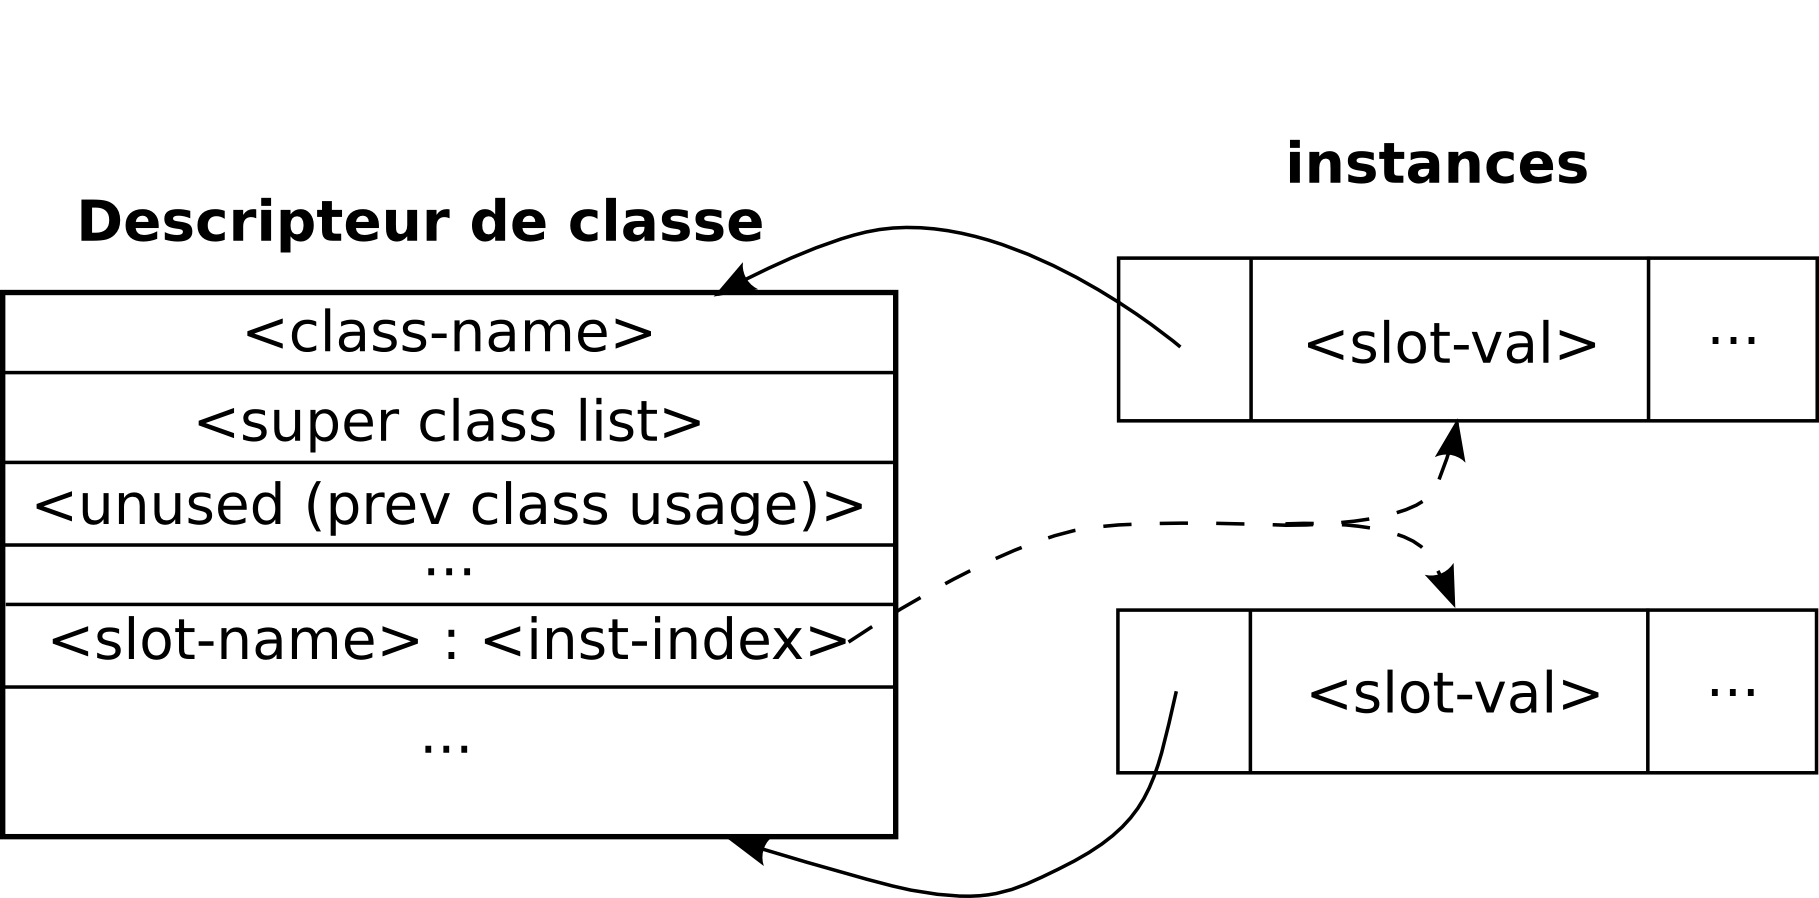
\includegraphics[scale=0.7]{oo-schema}
  \caption{Illustration des structures de données utilisées pour
    implanter l'exécution des classes et de leurs instances.}
  \label{OO:classdesc}
\end{figure}

Ainsi, l'endroit pour trouver l'index d'instance d'un champ donné
\emph{se trouve toujours au même endroit} dans tous les descripteurs
de classes. C'est ce qui permet de pouvoir utiliser les fonction
d'accès à un membre même avec une instance d'une sous-classe. Les
descripteurs de classes, tout comme les instances, sont implantés avec
des vecteurs Scheme afin d'avoir un accès rapide aux champs de ceux-ci.

Lorsque la forme spéciale \scheme{define-class} est expansée,
plusieurs informations sont extraites et traités afin de pouvoir
générer correctement les fonctions de création et d'accès aux
attributs. Entre autre, il faut obtenir la liste complète de tous les
attributs hérités par les classes parents à la classe décrite. Cette
information est stockée dans une table de hachage globale à
l'expansion macro nommée \scheme{mt-class-table} qui conserve
l'information disponible pour chaque classe déjà créées. Cette
information est aussi stockée sous forme de \emph{descripteurs de
  classes}, mais qui seront disponible uniquement pour l'expansion
macro. Ces derniers gardent trace du nom des classes créées, de leurs
hiérarchie et des indexes associés à leurs attributs. Ces indexes
correspondent à l'endroit dans les descripteurs de classes où l'on
trouvera les indexes d'indirection vers les instances.

Lorsque les nouveaux attributs (attributs non-hérités) sont inclus
dans descripteurs de classe de l'exécution, un compteur global
(expansion macro) est utilisé pour obtenir l'index du nouveau champs
dans le vecteur correspondant à ce descripteur. Un deuxième index,
local celui-ci, sera utilisé pour trouvé l'index de la position de
l'attribut dans l'instance. Ainsi, l'index global pointera vers
l'index d'instance dans le descripteur de classe. La création du
descripteur de classe pour l'expansion macro est donnée dans la figure
\ref{OO:classdesc-code}. Ce même objet sera recréé et utilisé comme
descripteur de classe durant l'exécution.

\begin{figure}[htb!]
  \begin{schemecode}
(let* ((instance-index 1) ; 0 -> class-desc
       (desc (make-class-desc
              name supers
              (if (pair? field-indices)
                  (- (slot-index
                      (cdar (take-right field-indices 1)))
                     1)
                  0))))
  (for-each
   (lambda (fi)
     (let ((index (slot-index fi)))
       (cond ((is-instance-slot? fi)
              (vector-set! desc index (instance-index++)))
             ((is-class-slot? fi)
              (vector-set! desc index 'unbound-class-slot))
             (else
              (error "Unknown slot type")))))
   (map cdr field-indices))
  desc)
  \end{schemecode}
  \caption{Création du descripteur de classe de l'expansion macro.}
  \label{OO:classdesc-code}
\end{figure}

Une fois cette information en main, toutes les fonctions d'accès et de
modification d'attributs peuvent être générées sans problèmes. La
plupart contiendront des indirections pour l'accès aux champs, sauf
pour les attributs de classes qui eux, se retrouvent directement dans
les descripteurs de classes. La figure \ref{OO:obj-struct} donne un
exemple concret de illustrant les structures utilisées lors de
l'exécution du système. On constate que le premier élément du vecteur
correspondant à l'instance créée est aussi un vecteur, qui lui,
correspond au descripteur de la classe \scheme{toto}. Le premier
élément de ce descripteur est le nom de la classe, le deuxième est la
liste des super classes par la suite viennent les indexes des
attributs dans l'instance. Par contre, puisque la classe \scheme{blub}
a été préalablement définie, le premier conteneur d'indirection a été
reservé pour le champs \scheme{b} de la classe \scheme{blub}. Ainsi,
l'indirection vers le champs \scheme{titi} se trouve dans le quatrième
éléments ($index = 3$) du descripteur. L'affichage de la fonction
d'accès au champs \scheme{titi} confirme bien ce fait et montre que la
valeur obtenue, en l'occurance 1, est utilisée comme index pour
obtenir la valeur du champs dans l'instance.

\begin{figure}[htb!]
  \begin{schemecode}
(define-class blub () (slot: b))
(define-class toto () (slot: titi) (class-slot: tutu))
(toto-tutu-set! 'allo!)
(new toto 12)
  \end{schemecode}
  \schemeresult{\#(\#(toto () unknown-slot 1 allo!) 12)}
  \begin{schemecode}
(pp toto-titi)
  \end{schemecode}
  \begin{verbatim}
(lambda (#:obj445)
  (vector-ref #:obj445
              (vector-ref (instance-class-descriptor #:obj445) 
                          3)))
  \end{verbatim}
  \caption{Exemple concret de structure d'instance, descripteur de
    classe et de fonction d'accès à un attribut par indirection.}
  \label{OO:obj-struct}
\end{figure}

Deux constructeurs d'instances sont finalement générés avec les
accesseurs. Le premier constructeur (\scheme{make-<class-name>})
construit et initialise \emph{tous} les champs d'une instance de la
même manière que procède le constructeur d'instance pour la forme
\scheme{define-type} de Gambit-C. Le deuxième
(\scheme{make-<class-name>-instance}) ne prend aucun argument et
produit une instance non-initialisée qui pourra être passée à
\scheme{init!}, la fonction générique d'initialisation d'objets. Par
défaut, une instance de cette fonction générique est créée, et fait
exactement le même travail que le premier constructeur. Aussi, une
fonction très rudimentaire d'introspection d'instance de classe est
aussi implantée sous la forme d'instances de la fonction générique
\scheme{describe}.


\subsection{Implantation de define-generic}

De manière similaire à la définition de nouvelles classes, des
informations sur les fonctions génériques définies et sur leurs
instances sont conservées dans une table de hachage globale durant
l'expansion macro et se nomme \scheme{mt-meth-table}. Ces informations
seront par la suite transférées vers l'exécution du programme sous la
forme de structures propres à chaque fonction génériques qui se
nomment \scheme{<genfun-name>-meth-table}. Ces structures contiennent
le nom de la fonction génériques, une table de hachage permettant de
vérifier rapidement l'existence d'une instance en utilisant le types
des arguments de cette fonction générique comme clé de la table et une
liste \emph{triée} des instances permettant d'accélérer le
polymorphisme de fonction génériques.

L'expansion macro de la définition d'une nouvelle fonction générique
résulte donc en la création de cette structure et en la création d'une
fonction, portant le nom de la fonction générique, qui a pour but de
faire le choix de la bonne instance, en fonction des paramètres qui
lui sont passés. La fonction de \textit{dispatch} générée pour la
fonction générique \scheme{init!} est illustrée dans la figure
\ref{OO:init!-gf}. Le code présenté a été légèrement modifié afin
d'illustrer uniquement l'essence du \textit{dispatch} effectué. On
constate que dans un premier temps, on cherche dans la table de
hachage de cette fonction générique si une instance associée aux types
des arguments passés (ou du \textit{cast} effectué) existe, et si ce
ne pas le cas, on cherche explicitement une instance admissible de
manière polymorphe à ces arguments.

\begin{figure}[htb!]
  \begin{schemecode}
(lambda (\#!key cast . args)
  (let ((types (cond ((pair? cast) cast) 
                     (else (map get-class-id args)))))
    (cond
      ((or (generic-function-get-instance init!-meth-table types))
           (find-polymorphic-instance? init!-meth-table 
                                       args types))
           => (lambda (method) 
                (apply (method-body method) args)))
      (else (error ...)))))
  \end{schemecode}
  \caption{Code expansé effectuant le \textit{dispatch} dynamique pour
    la fonction générique \scheme{init!}}
  \label{OO:init!-gf}
\end{figure}


L'algorithme qui détermine qu'elle instance est la plus spécifique
pour un ensemble d'argument donné est simple: On cherche a trouver la
première instance dont chacun des types est considéré équivalent au
type des arguments actuels \emph{dans une liste triée} des instances
en fonction spécificité. Le critère de spécificité est déterminé par
la profondeur dans la hiérarchie du type des arguments de l'instance,
\ie par la somme du nombre de classes parents pour chacun des types
des arguments passés. En ce qui concerne les types spéciaux comme
\scheme{match-value}, ces types sont considérés comme étant très
spécifiques et donc prioritaires à un simple correspondance du type
d'un objet. La figure \ref{OO:polymorphism} illustre le code utilisé
pour réalisé ce \textit{dispatch} polymorphique.

\begin{figure}[htb!]
  \begin{schemecode}
(define (find-polymorphic-instance? genfun actual-params actual-types)
  (let ((args-nb (length actual-params))
        (sorted-instances (generic-function-sorted-instances genfun)))
    (exists (lambda (method)
              (equivalent-types? (method-types method)
                                 actual-params
                                 actual-types))
            (filter (lambda (i) (= (length (method-types i)) args-nb))
                    sorted-instances))))
  \end{schemecode}
  \caption{Implantation de la recherche d'instances polymorphiques
    d'une fonction générique}
  \label{OO:polymorphism}
\end{figure}

Finalement, la fonction \scheme{call-next-method} fonctionne grâce au
mécanisme de variables dynamique fourni par Gambit-C. Une variable
dynamique interne (\scheme{\_\_\_call-next-method}) est utilisé pour
contenir un appel à la fonction générique appellée avec un
\textit{cast} spécial des arguments ou chaque argument est une liste
des super classes des types de l'instance actuellement
utilisée. Ainsi, lorsque cette appel est fait, l'on cherchera
l'instance polymorphique la plus spécifique pour ces types. Ainsi,
comme désiré, l'instance de cette fonction générique la plus
spécifique sera appelée

\subsection{Implantation de define-method}
L'expansion de la macro \scheme{define-method} est très simple, elle 
consiste en la création d'une structure de donnée qui contient le
corps de l'instance définie, ainsi que les types associés aux
arguments attendus. Cette structure existera durant l'expansion et
sera recréée lors de l'exécution du programme afin de pouvoir être
appelée par la fonction de \textit{dispatch}.




\section{Conclusion}
Ainsi un système objet complet a été développé dans le but d'étendre
le langage Scheme et d'y inclure les paradigme de la programmation
orientée objet. Ce système objet permet la déclaration de classes avec
héritage multiple et polymorphisme et de fonctions génériques
effectuant du \textit{dispatch} multiple. Ces choix de
caractéristiques ont été faite dans le but de donner le plus de
liberté aux programmeurs de jeux vidéo, tout en gardant en tête de
fournir de bonnes performances, tant en temps sur processeur qu'en
utilisation de la mémoire.

Les structures de données utilisées pour l'implantation d'objets sont
de tailles optimales, et ne requièrent qu'une indirection
supplémentaire afin de pouvoir accéder aux champs de ceux-ci. 

Les fonctions génériques utilisent des mécanisme de tri pré-calculé
afin d'accélérer le \textit{dispatch} d'instances de fonctions
génériques de manière polymorphe. 

Il serait maintenant très intéressant de modifier le système afin
qu'il supporte un protocole de méta objets. Un tel protocole donnerait
accès à une introspection très développée et permettrait aux
utilisateurs de modifier facilement le comportement du système selon
leurs besoins. 

Aussi, une modification du système afin de le rendre compatible avec
des objets de manière inter-modulaire serait une grande amélioration
en ce qui a attrait à la modularité du code. 

Par contre, une attention particulière devrait être portée aux coûts
en performance que ces modifications pourraient impliquer afin de
respecter la philosophie de base de ce système.



%%%%%%%%%%%%%%%%%%%%%%%%%%%%%%%%%%%%%%%%%%%%%%%%%%%%%%%%%%%%%%%%%%%%%%%%%%%%%%%
\chapter{Système de coroutines}
\todo{Système de threads offerts ne sont pas toujours
  satisfaisant. Mentalité Scheme: au lieu de contraindre ce qu'on veut
  faire en fonction de ce qui nous est offert, étendre le langage pour
  nous permettre de faire ce que l'on veut et surtout de la manière
  désirée.}

Le langage Scheme tel que décrit par le standard~\cite{R5RS} ne fourni
pas de système de \textit{threads}. Par contre, le document
\textit{Scheme Request For Implementation 18}~\cite{SRFI18} décrit un
\textit{API} de système de \textit{thread} concurrents. Le système
Gambit-C~\cite{Gambit4} supporte cet \textit{API} sous forme de
\textit{threads} verts. Ainsi, en plus d'avoir à utiliser les
mécanismes de synchronisations de \textit{thread} traditionnels afin
d'éviter les erreurs dues à la concurrence, aucun bénéfice en terme
d'accélération matérielle ne sera obtenu.

L'utilisation de \textit{threads} dans un jeu vidéo peut être très
pertinente et permettre de pouvoir exprimer de manière concise
beaucoup de concepts comme par exemple l'implantation de parties
multi-joueurs où ces derniers jouent à tours de rôles. Par contre, le
coût d'utiliser des synchronisation explicite est très élevé en temps
de développement et en utilisation du processeur lors de l'exécution. 

Par contre, un système de coroutines (appelé aussi \textit{threads}
coopératifs) permettrait d'éviter d'avoir à spécifier explicitement
ces synchronisations entre entités. En effet, si le flot de contrôle
est changé durant des moments opportuns, aucune synchronisation
supplémentaire n'est requise pour assurer des sections critiques. En
fait, le problème ne se pose même plus, mais disparaît
complètement. Ceci rend donc très attrayant de tels systèmes pour le
développement de jeux vidéo. Ils permettraient de pouvoir exprimer de
manière simple des changements de contextes dans le jeu, ou même, de
modulariser le comportement de chacune des entités du jeu.

Malheureusement, ni Scheme, ni Gambit-C n'offrent de tels système de
coroutines. Par contre, l'expressivité du langage Scheme, notamment
grâce à la réification de continuations rend la tâche tout à fait
accessible et réalisable. Ce chapitre vise donc à présenter un système
de \textit{threads} \emph{coopératifs} développé dans le but de aux
lacunes que présente le système de \textit{threads} offert par
Gambit-C en ce qui à attrait au développement de jeux vidéo.


\section{Description du langage}

Un système de \textit{threads} coopératifs implique donc que le
changement de contexte d'exécution associé aux changement de
\textit{threads} doit être fait de manière explicite par les
utilisateurs. Ces \textit{threads} coopératifs sont aussi connus sous
le nom de coroutines. Ainsi, ces changements de contextes peuvent être
faits aux moments opportuns, assurant ainsi l'intégrité des données.

Une synchronisation entre les différents \textit{threads} sera encore
nécessaire afin qu'ils puissent bien être orchestrer, mais les
synchronisation similaire aux section critiques ne seront plus
nécessaires. Afin de permettre aux coroutines de pouvoir communiquer
entre elles, une synchronisation par passage de message avec
\textit{pattern matching} à la Termite~\cite{Termite_paper} a été
adoptée. Ce mécanisme permet de pouvoir synchroniser de manière
élégante

De plus, le système a été conçu afin de permettre d'être utilisé de
manière récursive. Il est donc possible d'avoir une coroutine qui sera
elle-même un système de coroutine, et ainsi de suite. Cette
fonctionnalité a été implantée de manière à ce que le système soit le
plus générique possible. De plus, l'idée de système récursifs est
aussi très près du langage Scheme dans lequel la récursion de
fonctions est très courante et commune grâce à l'implantation de
l'optimisation d'appels terminaux.

Aussi, la notion de temps a été abstraite dans le système avec
l'introduction de compteurs de temps (\textit{timers}). Il est donc
possible de choisir non seulement une granularité temporelle en
spécifiant la fréquence de se compteur de temps, mais il est aussi
possible de spécifier un facteur d'accélération, permettant de pouvoir
accélérer la simulation en cours.

Le système se résume à un schéduleur de coroutine qui utilise une file
de coroutines prêtes pour choisir la prochaine coroutine à exécuter, à
une file de coroutine en attente sur le temps et à des coroutine en
attente de conditions, comme de la réception d'un message par
exemple. Lorsqu'une coroutine décide de passer la main à une coroutine
suivante ou lorsqu'elle ne doit plus attendre après le temps ou une
condition, elle se fait enfiler à la fait de la file d'attente de
coroutines prêtes. La figure \ref{Corout:system-schema} illustre
l'architecture globale du système.

\begin{figure}[htb!]
  \center
  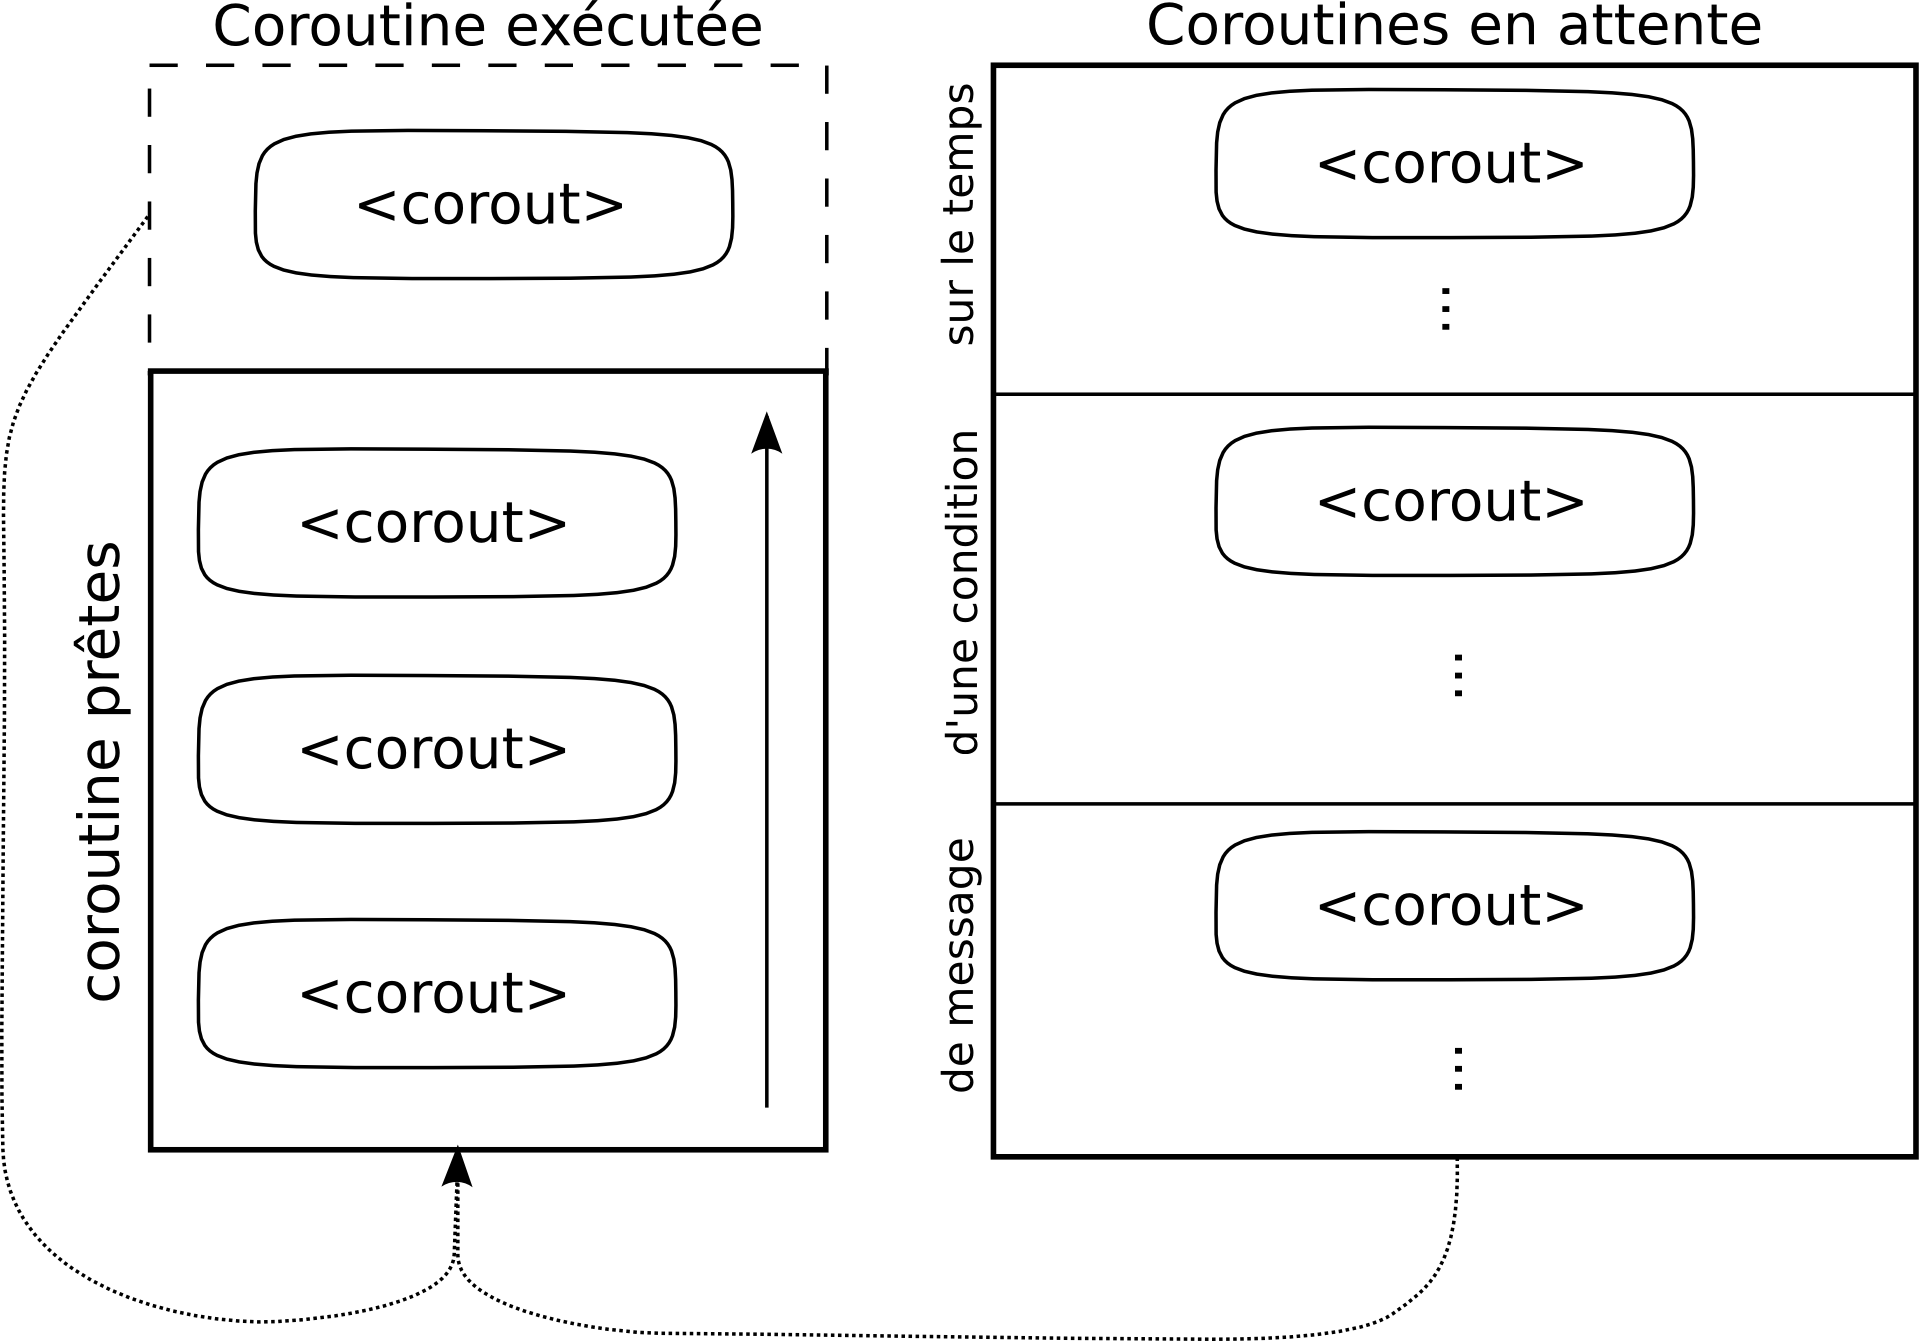
\includegraphics[scale=0.7]{corout-system}
  \caption{Architecture globale du système de coroutine}
  \label{Corout:system-schema}
\end{figure}

 Les sections suivantes décrivent un \textit{API} permettant
l'utilisation du système de coroutines créé.


\subsection{Création de coroutines}
Les coroutines sont des objets en eux même et peuvent être créés de
manière externe au système de coroutines pour, par la suite, être
intégrées à celui-ci. L'avantage de cette approche, utilisée aussi par
le système de \textit{threads} de Gambit-C, réside dans le fait que
les objets correspondant aux \textit{threads} peuvent être préparés à
l'avance et conservés jusqu'au moment opportun de leurs intégration
dans le système. Une nouvelle instance de coroutine s'effectue avec

\begin{schemecode}
(new corout <corout-id> <thunk>)
\end{schemecode}

\noindent
où \scheme{<corout-id>} est un symbol permettant d'identifier la
coroutine et le dernier argument est une fonction prenant aucun
argument (appelée aussi \textit{thunk}), qui contient le corps de
l'exécution de cette coroutine.

L'objet créé pourra être par la suite intégré à un nouveau système par
les fonctions d'initialisations \scheme{boot} et \scheme{simple-boot}
ou encore intégrés à une coroutine d'une simulation existante avec la
fonction \scheme{spawn-brother}. Ces fonction sont décrites plus bas.

Finalement, il est possible de rendre une coroutine prioritaire ou non
prioritaire en utilisant les fonctions \scheme{(prioritize! <corout>)}
et \scheme{(unprioritize! <corout>)}. Lors de leurs création, toute
les coroutines sont considérées comme étant non
prioritaire. Lorsqu'une coroutine devient prioritaire, elle sera
automatiquement \emph{la prochaine} a être exécutée lors d'un
changement de coroutine. Il est donc important que cette coroutine
enlève sa priorité pour éviter des boucles infinies par la suite.

\subsection{Démarrage du système}

Le système de coroutines peut être démarrer en utilisant la fonction 

\begin{schemecode}
(boot <timer> <return-val-handler> <corout1> ...)
\end{schemecode}

\noindent
dont le premier argument doit être un objet correspondant à un
compteur de temps pour le système, le deuxième paramètre est une
fonction permettant la gestion des valeurs de retours des coroutines
et par la suite viennent les coroutines qui seront présentent au
démarrage du système créé. L'ordre de ces coroutines est significatif
: il indique dans quel ordre seront exécutées les coroutines.

La création de \textit{timers} se fait par un appel à la fonction 

\begin{schemecode}
(start-timer! <period> [time-multiplier: <time-mult-value>]))
\end{schemecode}

\noindent
qui s'occupe de créer un objet faisant abstraction du temps avec une
granularité associé à la période (en secondes) spécifiée. La fonction
\scheme{(stop-timer! <timer>)} doit être utilisée afin d'arrêter le
compteur de temps, lorsque son utilisation n'est plus nécessaire.

La fonction s'occupant de gérer les valeurs de retour des coroutines
se doit de recevoir deux arguments, le premier étant le résultat
accumulé des précédentes terminaisons de coroutines et le deuxième
étant la valeur de retour de la dernière coroutine à avoir terminer
son exécution. La valeur de retour de cette fonction sera alors
utilisée comme la prochaine valeur accumulée lors de la terminaison
subséquente d'une coroutine, comme c'est le cas avec la fonction
\scheme{fold} (voir la figure \ref{Scheme:fold}).

La figure \ref{Corout:boot} présente un exemple de démarrage d'un
système de coroutine où le temps sera augmenté toutes les secondes et
où le résultat finale de la simulation sera la somme des valeurs
retournées par chacune des coroutines. Il est important de noter qu'il
ne faut pas oublier d'arrêter le \textit{timer} lorsqu'il n'est plus
nécessaire.

\begin{figure}[htb!]
  \begin{schemecode}
(let* ((c1 (new corout 'c1 (lambda () 1)))
       (c2 (new corout 'c2 (lambda () 2)))
       (c3 (new corout 'c3 (lambda () 3)))
       (timer (start-timer! 1.0))
       (result (boot timer + c1 c2 c3)))
    (stop-timer! timer)
    result)
  \end{schemecode}
  \schemeresult{6}
  \caption{Exemple de démarrage d'un système de coroutines}
  \label{Corout:boot}
\end{figure}

Le processus de démarrage peut être simplifié avec l'utilisation de la
fonction \scheme{(simple-boot <corout1> ...)} qui utilise un
\textit{timer} par défaut avec une période de $0.001$ secondes et
retourne la valeur de la dernière coroutine à être exécutée dans le
système comme valeur de retour du système. La figure
\ref{Corout:simple-boot} illustre le démarrage d'un système de
coroutines en utilisant \scheme{simple-boot}. 

\begin{figure}[htb!]
  \begin{schemecode}
(let* ((c1 (new corout 'c1 (lambda () 1)))
         (c2 (new corout 'c2 (lambda () 2)))
         (c3 (new corout 'c3 (lambda () 3))))
    (simple-boot c1 c2 c3))
  \end{schemecode}
  \schemeresult{3}
  \caption{Exemple de démarrage simple de système de coroutines}
  \label{Corout:simple-boot}
\end{figure}


\subsection{Manipulation du contrôle de flot}
Puisque le contrôle du flot d'exécution entre les coroutines doit être
explicité par l'utilisateur, une bonne diversité de fonctions
permettent la manipulation de celui-ci. Il est important de noter que,
sauf avec avis contraire, toutes les fonctions décrites dans cette
section doivent être exécutée \emph{par} une coroutine, \ie dans leur
corps.

La fonction la plus simple de manipulation du flot d'exécution est
\scheme{(yield)}. Celle-ci arrête temporairement la coroutine actuelle
et passe le contrôle à la \emph{prochaine} coroutine disponible. La
prochaine coroutine sera déterminée de manière déterministe avec une
simple file d'attente. La coroutine actuelle sera donc placée à la fin
de cette file d'attente (à moins d'être prioritaire). Ainsi, le retour
du contrôle à cette coroutine ne sera exécutée uniquement lorsque
toutes les autres coroutines prêtes auront décidée de passer la main à
la coroutine suivante. Il est également possible de choisir
explicitement à quelle coroutine le contrôle sera passé avec la
fonction:

\begin{schemecode}
(yield-to <corout> [for: <sec>] [forced-yield: <thunk>])
\end{schemecode}

\noindent
Cette fonction possède aussi une particularité intéressante. Elle
permet aussi, si spécifié, de limiter en temps l'exécution de la
coroutine. Cette particularité doit, par contre, être utilisée avec
modération car elle brime l'atomicité du système qui est garantie avec
les autres fonctions de changement de contexte. Elle permet ainsi de
pouvoir exécuter une coroutine qui n'interfère pas avec les autres,
tout en contrôlant l'étendu du calcul de celle-ci. Le mot clé
\scheme{forced-yield:} permet, quant à lui, spécifier la fonction qui
sera utilisé pour effectuer le changement de contexte forcé de cette
coroutine. La figure \ref{Corout:yield-to-ex} illustre un exemple
d'utilisation.

\begin{figure}[htb!]
  \begin{schemecode}
(let* ((c1 (new corout 'c1 (lambda () (write 1))))
       (c2 (new corout 'c2 (lambda ()
                             (yield-to c1 for: 0.1
                                       forced-yield:
                                         (lambda () (recv (go 'ok))))
                             (fib 32) (write 2) (! c1 'go))))
       (c3 (new corout 'c3 (lambda () (fib 32) (write 3)))))
  (simple-boot c2 c3))
  \end{schemecode}
  \schemeresult{132}
  \caption{Exemple d'utilisation de la fonction \scheme{yield-to}}
  \label{Corout:yield-to-ex}
\end{figure}

Une coroutine peut aussi décider de se mettre en attente pour une
certaine période de temps avec la fonction \scheme{(sleep-for <sec>)}
un certain nombre de secondes. Il en résultera que la coroutine
actuelle sera placée dans une file d'attente séparée et ne sera
ré-enfilée dans la file de coroutines prêtes uniquement lorsque le
délais prescrit sera dépassé. Cela n'implique pas que la coroutine
sera exécutée à ce moment là, car si cette file contient déjà des
coroutines en attentes, elle devra attendre sont tour pour pouvoir
poursuivre son exécution.

Il est également possible pour une coroutine d'intégrer des nouvelles
coroutines dans le système en utilisant les fonctions:

\begin{schemecode}
(spawn-brother <corout>)
(spawn-brother-thunk <corout-id> <thunk>)
\end{schemecode}

La première intégrera simplement la coroutine spécifiée dans la file
de coroutines prêtes. Cette coroutine \emph{ne doit pas} déjà être
présente dans le système. La deuxième fonction,
\scheme{spawn-brother-thunk} créera une nouvelle coroutine ayant comme
identificateur \scheme{<corout-id>} et la fonction spécifiée comme
corps et sera, par la suite, intégrée de même manière dans le système.

Une coroutine peut aussi altérer le fil de son exécution en modifiant
la continuation de son calcul par celui d'une autre coroutine ou d'un
\textit{thunk} (fonction sans argument) de manière similaire à la
forme spéciale \scheme{call/cc} de Scheme. Ainsi, un appel à la forme
spéciale \scheme{(continue-with <corout>)} fera en sorte que la
continuation de la coroutine devienne celle de cette autre
coroutine. De manière similaire, \scheme{(continue-with-thunk!
  <thunk>)} utilisera la fonction passée comme continuation du
calcul. La figure \ref{Corout:cont-mod} présente un exemple utilisant
ces deux formes spéciales. Lorsque la coroutine \scheme{c1} s'exécute,
sa continue change pour celle de \scheme{c2} qui change à sont tour
pour la fonction \scheme{t}. Ainsi, les suites des coroutines
\scheme{c1} et \scheme{c2} ne sont jamais exécutés puisque leurs
continuation ont été altérées.

\begin{figure}[htb!]
  \begin{schemecode}
(let* ((t (lambda () (pp 'bonjour) 0))
       (c2 (new corout 'c2
                (lambda () (continue-with-thunk! t) (pp 'allo ) 2)))
       (c1 (new corout 'c1
                (lambda () (continue-with c2) (pp 'salut) 1))))
  (simple-boot c1))
  \end{schemecode}
  {{\it
bonjour\\
0}}
  \caption{Exemple de modification de la continuation d'une coroutine}
  \label{Corout:cont-mod}
\end{figure}

Finalement, une coroutine peut changer sa continuation de manière plus
drastique en forçant la terminaison du fil d'exécution de celle-ci en
utilisant la fonction \scheme{(terminate-corout <return-val>)}. La
valeur de retour de la coroutine sera alors la valeur spécifiée en
paramètre. Il est aussi possible de faire terminer le système actuel
de coroutine, au complet, en faisant appel à \scheme{(kill-all!
  <return-val>)}. La valeur de retour finale de l'exécution du système
sera alors la valeur spécifiée.



\subsection{Environnement dynamique}
Un environnement dynamique est disponible pour les coroutines, lors de
leurs exécution. Cet environnement donne accès à de l'information sur
ce dernier. il comprend les paramètres:

\begin{itemize}
\item \scheme{(current-corout)} : retourne l'instance de la coroutine
  actuellement exécutée. 

\item \scheme{(timer)} : retourne l'objet d'abstraction du temps
  associé avec le système courant. La valeur actuelle du temps peut
  être obtenue facilement en appellent plustôt la fonction
  \scheme{(current-sim-time)}.

\item \scheme{(return-value)} : Valeur de retour accumulée des
  coroutines au moment de l'appel.
\end{itemize}



\subsection{Système de communication inter coroutines}
Le mécanisme principal de synchronisation des coroutines est basé sur
le passage de message, tel que fait dans le système de programmation
distribué Termite~\cite{Termite_paper}. Cette approche semble
naturelle pour la programmation de jeux vidéo où les coroutines
peuvent devenir des entités à part entière et pourraient ainsi
communiquer avec d'autres entités par ces mécanismes d'une manière
naturelle.

L'envoi de message se fait par la fonction \scheme{(! <corout> <msg>)}
qui s'occupe d'acheminer le message désiré à la coroutine spécifiée.

La réception de messages peut se faire avec deux fonctions distinctes
ou une forme spéciale:

\begin{itemize}
\item \scheme{(? [timeout: <sec>])} : Réception du premier message
  disponible avec attente bloquante. Un \textit{timeout} peut être
  spécifié afin de limiter l'attente faite. Si plusieurs messages sont
  disponible, le premier arrivé sera alors retourné, afin de respecter
  une politique équitable de réception de messages.

\item \scheme{(?? <predicat> [timeout: <secs>])} : Réception du
  premier message qui retourne vrai, selon le prédicat spécifié. Le
  prédicat doit prendre un seul argument, un message reçu. Comme pour
  la fonction \scheme{?}, l'attente bloquante peut être interrompue
  après un délais de temps, si ce dernier est spécifié.

\item \scheme{(recv (<pattern> <body>) ...)} : Cette forme spéciale
  permet la réception sélective de messages selon des patrons de
  filtrage par motifs (\textit{pattern matching}). Ces patrons
  permettent de pouvoir facilement exprimer la forme attendue du
  message et de pouvoir lier des variables locales à des parties du
  messages reçu et les utiliser dans le corps du patron. Lorsque
  plusieurs messages reçus peuvent correspondre aux motifs donnés, la
  sélection du message se fait en choisissant dans un premier temps le
  premier motifs possible, et par la suite le premier message
  répondant à ce motif. Ainsi l'ordre de spécification des motifs est
  importante et significative.

\end{itemize}

Les valeurs de délais d'attentes maximums spécifiés pour la réception
de messages impliquent qu'il est possible qu'une réception
échoue. Dans un tel cas, une exception de type
\scheme{mailbox-timeout-exception} est lancée par la fonction de
réception utilisée.

Les patrons utilisé dans le filtrage de motifs de la forme spéciale
\scheme{recv} diffèrent de ceux dans Termite. Ici, le patron doit être
une donnée Scheme. Lorsque, dans cette donnée, un symbole est précédé
d'une virgule (\textit{unquote}), le symbole est \emph{lié} à la
valeur trouvée à cet endroit du motif dans le message reçu. Les
formats de motifs reconnus sont les symboles, les mots clés, les
caractères, les valeurs booléennes, les nombres, les chaînes de
caractères, les listes et les vecteurs. La figure
\ref{Corout:recv-pat} illustre plusieurs motifs différents qui peuvent
être utilisés.

\begin{figure}[htb!]
  \begin{schemecode}
(recv (salut 'got-salut)                   ; symbol match
      ("bonjour" 'bonjour)                 ; strng match
      (1011 '11-or-1011?)                  ; number match
      ((a ,b c) (string b \#\textbackslash k))           ; list match
      (\#(a b ,c) c)                        ; vector match
      ((tata 1 \#(toto ,x) "titi") (+ x 1)) ; complex match
      (,anything anything))                ; can match anything
  \end{schemecode}
  \caption{Exemple de patrons pouvant être utilisés dans le filtrage
    par motifs de la forme spécial \scheme{recv}}
  \label{Corout:recv-pat}
\end{figure}

Une particularité intéressante de ce filtrage par motif reliée au fait
qu'il est possible d'utiliser des patrons de manière dynamique, \ie
qui n'apparaissent pas dans la forme spéciale, mais plutôt qui ont été
spécifiés grâce à la forme spéciale \scheme{(with-dynamic-handlers
  ((<pattern> <handler-body>) ...) <body>)}. Tous les appels à la
forme spéciale \scheme{recv} se trouvant dans le corps
(\scheme{<body>}) se trouveront augmenter de ces nouveaux patrons,
mais ces derniers seront considérés en dernier lieu. Il est donc
possible ainsi de pouvoir factoriser des patrons communs et de les
appliquer à tous les appels de la forme spéciale de réception de
message par filtrage de motifs.

Aussi, un mécanisme de liste de diffusion a été inclus. Ce mécanisme
simple permet d'enregistrer des coroutine dans une liste de diffusion
et, par la suite, d'envoyer à toutes les coroutines inscrite des
messages de manière simultanée. Quoi que très primitif, ce système
permet d'émuler la base de système de programmation
réactive~\cite{FRP}. Les fonctions de gestion et d'utilisation de
listes de diffusions sont:

\begin{itemize}
\item \scheme{(subscribe <list-id> <corout>)} : Inscription de la
  coroutine spécifiée à la liste de diffusion identifiée par le symbole
  choisi. Si la liste n'existait pas, elle sera créée.

\item \scheme{(unsubscribe <list-id> <corout>} : Désinscription d'une
  coroutine à une liste de diffusion.

\item \scheme{(broadcast <list-id> <msg>)} : Envoi d'un message à une
  liste de diffusion.
\end{itemize}

\subsection{Autres mécanismes de synchronisation}
En plus du mécanisme de messagerie sophistiqué du système de
coroutine, les coroutines disposent d'un système de sémaphores afin de
pouvoir exécuter des synchronisation de manière plus
traditionnelle. Ces dernières sont manipulés par les fonctions:

\begin{itemize}
\item \scheme{(new-semaphore <init-value>)} : Création d'une nouvelle
  sémaphore ayant comme valeur initiale \scheme{<init-value>}.

\item \scheme{(new-mutex)} : Création d'une nouvelle sémaphore ayant
  comme valeur initiale 1.

\item \scheme{(sem-locked? <sem>)} : Permet de vérifier s'il reste des
  ressources disponibles dans une sémaphore. S'il en reste, la
  fonction retournera vrai, ou faux sinon.

\item \scheme{(sem-lock! <sem>)} : Prend une ressource de la sémaphore
  spécifiée. Si aucune ressource n'est disponible, la coroutine se met
  en étant d'attente bloquante jusqu'à ce qu'une ressource soit
  libérée.

\item \scheme{(sem-unlock! <sem>)} : Libère une ressource de la
  sémaphore spécifiée. Aucune vérification n'est faite qu'en a
  s'assurer que la coroutine courante possède réellement cette
  ressource. Si des coroutines sont en attentes de ressources, la
  première à s'être mise en attente est alors réveillée.
\end{itemize}

L'utilisation de sémaphores n'est pas nécessaire, puisque
l'utilisation du système de messagerie permet d'effectuer n'importe
qu'elle synchronisation. Par contre, les sémaphores permettent de
pouvoir exprimer d'une manières différente des synchronisations et
donc donnent plus de liberté aux utilisateurs du système.

\subsection{Systèmes en cascades}

Le système de coroutine a été conçu de manière à pouvoir permettre de
créer des systèmes coroutines de manière cascadée, \ie de créer des
coroutines qui sont elles-mêmes des système de coroutines. La
procédure de création de ces derniers est simple, il ne suffit que de
démarrer un nouveau système de coroutine à l'intérieur d'une coroutine
existante. Par contre, un problème se pose: il devient alors
impossible de pouvoir retourner le contrôle aux coroutines appartenant
au système primordial, puisque \scheme{(yield)} ne fera que changer de
contexte que les coroutines du sous-système.

Ce problème est résolu par l'utilisation de la fonction
\scheme{(super-yield)} qui effectue un changement de contexte pour le
système de coroutine courant. Si le système courant ne se retrouve pas
dans un système cascadé, alors rien ne se produira. Une fonction
similaire, \scheme{(super-kill-all! <return-value>)} terminera
\emph{tous} les systèmes de coroutines se retrouvant dans
l'arborescence de système de coroutine présentement active. Un exemple
de système de coroutines en cascade est donné dans la figure
\ref{Corout:cascade}.  On constate que les appels à
\scheme{super-yield} ont bien effectué les changements de contextes de
des coroutines hôtes des sous-systèmes de coroutines (\scheme{s1} et
\scheme{s2}).

\begin{figure}[htb!]
  \begin{schemecode}
(let* ((ret (lambda (x) (pp `(now returning: ,x)) x))
       (c1 (new corout 'c1 (lambda () (ret 1))))
       (c2 (new corout 'c2 (lambda () (super-yield) (ret 2))))
       (c3 (new corout 'c3 (lambda () (ret 3))))
       (c4 (new corout 'c4 (lambda () (ret 8))))
       (c5 (new corout 'c5 (lambda () (super-yield) (ret 4))))
       (c6 (new corout 'c6 (lambda () (ret 2))))
       (timer (start-timer! 1.0))
       (s1 (new corout 's1 (lambda () (boot timer + c1 c2 c3))))
       (s2 (new corout 's2 (lambda () (boot timer - c4 c5 c6)))))
  (boot timer * s1 s2))
  \end{schemecode}
  {{\it
(now returning: 1)\\
(now returning: 8)\\
(now returning: 2)\\
(now returning: 3)\\
(now returning: 4)\\
(now returning: 2)\\
12}}
  \caption{Exemple de démarrage de système de coroutines en cascade}
  \label{Corout:cascade}
\end{figure}




\section{Implantation}

L'implantation de ce système de coroutine est centralisée sur
l'utilisation de la forme spéciale \scheme{call/cc} afin de permettre
la conservation de l'état courant d'une coroutine.

Un net avantage lorsque le système est directement implanté par
l'utilisateur est qu'il répond sur mesure aux demandes de ce dernier
et donc il peut s'exprimer dans une syntaxe simple, tout en conservant
un contrôle fin sur le comportement du système.

Cette section explique les mécaniques internes du système de
coroutines développé, en expliquant non seulement les structures de
données utilisées, mais aussi les algorithmes utilisés.

\subsection{Implantation des coroutines}

La structure de donnée des coroutine est implantée en utilisant le
système d'objets présenté dans le chapitre \ref{Chap:OO}. La structure
employée est illustrée dans la figure \ref{Corout:corout-class}. Elle
contient toutes les informations essentielles au fonctionnement de
celle-ci, dont entre autre sa continuation (\scheme{kont}), sa boîte
de messagerie, une sauvegarde de l'environnement d'un sous-système de
coroutine (\scheme{state-env}), etc... 

\begin{figure}[htb!]
  \begin{schemecode}
(define-class corout ()
  (slot: id)
  (slot: kont)
  (slot: mailbox)
  (slot: state-env) ;; should be unprintable
  (slot: prioritize?)
  (slot: sleeping?)
  (slot: delta-t)
  (slot: msg-lists)
  (constructor:
   (lambda (obj id thunk)
     (set-fields! obj corout
       ((id          id)
        (kont        (lambda (dummy) (terminate-corout (thunk))))
        (mailbox     (new-queue))
        (state-env   \#f)
        (prioritize? \#f)
        (sleeping?   \#f)
        (delta-t     \#f)
        (msg-lists   (empty-set)))))))
  \end{schemecode}
  \caption{Structure de donnée représentant une coroutine}
  \label{Corout:corout-class}
\end{figure}

La continuation primordiale d'une coroutine est sa terminaison de
manière \og propre \fg, \ie en utilisant la fonction de terminaison de
coroutines. C'est ce qui permet à une coroutine ayant comme corps
uniquement \scheme{(lambda () 1)} de terminer correctement avec la
valeur de retour 1.

La variable d'état \scheme{sleeping?} permet d'indiquer à
l'ordonnanceur de savoir si la coroutine qui vient de céder le
contrôle a été mise en veuille ou non, afin de savoir si cette
dernière doit retourner dans la file d'attente des coroutine prêtes.

\subsection{Timers}
Les timers sont aussi implantés comme des instances d'une classe
appartenant au système objet du chapitre \ref{Chap:OO}. Leurs rôle est
de fournir une abstraction temporelle pour le déroulement du système
de coroutines, qui peut être perçu comme une simulation. Cette classe
très simple contient des champs afin de garder compte du temps courant
de la simulation, de la période du timer, etc... 

Les timers doivent être rafraîchis régulièrement selon une période
fixe, ainsi il doivent être exécutés complètement à l'extérieur du
système de coroutine pour y arriver et donc, sont implantés en
utilisant le système de \textit{threads} de Gambit-C. Il en résulte
donc que ces derniers sont rafraîchis régulièrement de manière
concurrente avec le système de coroutines.

\subsection{Ordonnancement}
L'ordonnancement est le coeur du système de coroutine. Cet
ordonnancement évolue dans un environnement dynamique contenant l'état
du système de coroutines actif. Cet environnement dynamique comprend
les paramètres:

\begin{itemize}
\item \scheme{current-corout} : Paramètre contenant la coroutine
  actuellement exécutée. Lorsque celle-ci termine sont exécution, sa
  valeur de retour doit être placée dans ce paramètre pour signaler à
  l'ordonnanceur la terminaison de la coroutine.
\item \scheme{q} : File d'attente des coroutines prêtes à être
  exécutée (\textit{ready queue}).
\item \scheme{timer} : \textit{Timer} utilisé pour la simulation.
\item \scheme{time-sleep-q} : File prioritaire implantée avec un arbre
  rouge-noire qui contient les coroutines en attentes sur le temps.
\item \scheme{root-k} : Continuation primordiale, \ie continuation de
  du système de coroutine courant.
\item \scheme{return-value-handler} : Fonction utilisée pour accumuler
  les résultats de terminaison des coroutines.
\item \scheme{return-value} : Accumulateur de valeurs de retours des
  coroutines terminées.
\item \scheme{parent-state} : Sauvegarde de l'état du système de
  coroutine \emph{parent} au système actuel, dans des système
  cascadés. Cet état est décrit par les paramètres présentés ici.
\item \scheme{return-to-sched} : Continuation de l'ordonnanceur
\item \scheme{dynamic-handlers} : Liste de patrons dynamiques utilisés
  avec la forme spéciale \scheme{recv}.
\item \scheme{sleeping-coroutines}: Nombres de coroutines en
  attentes. Cette variable est nécessaire parce que l'accès aux files
  \scheme{q} et \scheme{time-sleep-q} n'est pas suffisante. En effet,
  les coroutines peuvent être en attente sur des mutex ou sur eux-même
  (reception d'un message), ainsi ce paramètre permet à l'ordonnanceur
  de savoir s'il existe toujours au moins une coroutine en attente.
\end{itemize}

La récursion de système fonctionne grâce à un système de sauvegarde
de cet état dans le paramètre \scheme{parent-state} dans un sens ou
dans le champs \scheme{state-env} d'un objet de coroutine dans
l'autre.

L'algorithme d'ordonnancement, en lui même, est très simple. Ce
dernier est présenté intégralement dans la figure
\ref{Corout:scheduler}. Dans un premier temps, la valeur de retour de
la coroutine précédente, si cette dernière a terminée, est traité ou
dans le cas échéant, elle est automatiquement remise dans la file
d'attente des coroutines prêtes. Par la suite, la file prioritaire de
coroutines en attente sur le temps est regardée afin réveiller toutes
coroutines ayant dépassé sont délais de sommeil. Finalement, la
première coroutine disponible dans la file de coroutines prêtes est
choisie comme prochaine coroutine et sont travail est poursuivi par un
appel à \scheme{resume-coroutine}. Si aucune coroutine ne se trouvait
dans la file \scheme{q}, alors une vérification des coroutines en
attente sur le temps est faite afin de déterminer s'il reste du
travail à faire. S'il y a des coroutine en attente sur le temps, alors
l'ordonnanceur se met en veille pour le délais d'attente
restant. Cette particularité se distingue nettement des simulations à
événements discrets qui auraient plutôt incrémentés leur horloge
interne directement de ce délais, chose qui est indésirable pour un
jeu vidéo. Par contre, si aucune coroutine n'est prête ou ne dort sur
le temps, alors le système ne peut plus rien faire. S'il existe
d'autres coroutines en veille (par exemple sur l'attente d'un
message), alors le système est un interblocage. Sinon, alors le
travail est terminé et donc, l'état du système parent est rétabli et
la continuation primordiale est invoquée.

\begin{figure}[htb!]
  \begin{schemecode}
(define (corout-scheduler)
    (manage-return-value)
    (wake-up-sleepers)
    (current-corout (dequeue! (q)))
    (cond
     ((corout? (current-corout))
      (resume-coroutine)
      (corout-scheduler))
     ((not (time-sleep-q-empty? (time-sleep-q)))
      (let* ((next-wake-time
              (time-sleep-q-el-wake-time
               (time-sleep-q-peek? (time-sleep-q)))))
        (thread-sleep! (/ (- next-wake-time (current-sim-time))
                          (timer-time-multiplier (timer)))))
      (current-corout \_\_\_scheduler-is-speeping\_\_\_)
      (corout-scheduler))
     (else
      (let ((finish-scheduling (root-k))
            (ret-val (return-value)))
        (if (> (sleeping-coroutines) 0)
            (error "Deadlock detected in coroutine system..."))
        (restore-state (parent-state))
        (continuation-return finish-scheduling ret-val)))))
  \end{schemecode}
  \caption{Algorithme d'ordonnancement}
  \label{Corout:scheduler}
\end{figure}

Le changement de contexte et le retour au contexte d'une coroutine
sont fait, à la base, par les fonctions \scheme{yield} et
\scheme{resume-coroutine}, illustrée respectivement dans les figure
\ref{Corout:yield} et \ref{Corout:resume-corout}. La figure
\ref{Corout:yield} illustre aussi la version permettant le changement
de contexte du système de coroutine. Ces fonctions illustre la base
même du système de coroutine, où la réification de continuations
permet la sauvegarde de l'état présent du calcul pour une utilisation
future. Comme l'indique la figure \ref{Corout:resume-corout}, l'état
de ces calculs sont poursuivis simplement par l'appel de ces
continuations sauvegardées dans la structure de donnée des
coroutine. Il est important de préciser que l'ordre dans lequel les
états des systèmes de continuations (pour des systèmes récursifs) sont
sauvegardés et restaurés est critique afin du bon fonctionnement de
ces appels. Par exemple, lors d'un appel à \scheme{super-yield},
l'état du système actuel doit absolument être sauvegardé avant de
restauré l'état du système parent pour éviter de le perdre.

\begin{figure}[htb!]
  \begin{schemecode}
(define (yield)
  (continuation-capture
   (lambda (k)
     (corout-kont-set! (current-corout) k)
     (resume-scheduling))))
(define (super-yield)
  (continuation-capture
   (lambda (k)
     (if (parent-state)
         (let ((state (save-state)))
           (restore-state (parent-state))
           (corout-state-env-set! (current-corout) state)
           (corout-kont-set! (current-corout) k)
           (resume-scheduling))))))

  \end{schemecode}
  \caption{Fonctions de changement de contexte explicite}
  \label{Corout:yield}
\end{figure}

\begin{figure}[htb!]
  \begin{schemecode}
(define (resume-coroutine)
  (continuation-capture
   (lambda (k)
     (return-to-sched k)
     (let ((kontinuation (corout-kont (current-corout))))
       (if (corout-state-env (current-corout))
           (let ((state (save-state)))
             (restore-state (corout-state-env (current-corout)))
             (parent-state state)))
       (continuation-return kontinuation 'go)))))
  \end{schemecode}
  \caption{Implantation du retour au contexte d'une coroutine}
  \label{Corout:resume-corout}
\end{figure}

La fonction \scheme{yield-to}, présentée dans la figure
\ref{Corout:yield-to}, diffère des autres fonctions de changement de
contexte, puisqu'elle permet aux utilisateurs de s'assurer que
l'exécution d'une coroutine ne dépassera pas un certain délais de
temps donné. Cette particularité a été implantée grâce à l'utilisation
des \textit{threads} de Gambit-C. Lorsqu'un délais maximal est
spécifié, un \textit{thread} secondaire est démarré est effectuera une
attente du délais prescrit de manière parallèle au système de
coroutine. Lorsque le délais est dépassé, il vérifie alors si la
coroutine exécutée est celle utilisée dans l'appel à \scheme{yield-to}
et si c'est le cas, il force cette coroutine a effectuer un appel de
changement de contexte qui peut être choisi par l'usager. Ce
changement de contexte forcé est possible grâce à la fonction
\scheme{thread-interrupt!} de Gambit-C qui permet au \textit{thread}
auxiliaire de force l'évaluation d'un \textit{thunk} dans
l'environnement du \textit{thread} exécutant le système de coroutines.

\begin{figure}[htb!]
  \begin{schemecode}
(define (yield-to corout \#!key (for \#f) (forced-yield yield))
  (let* ((interupt-body
          (lambda () (if (eq? (current-corout) corout) (forced-yield))))
         (timer-body
          (lambda ()
            (thread-sleep! (/ for (timer-time-multiplier (timer))))
            (thread-interrupt! (current-thread) interupt-body)))
         (timer-thread
          (and for
               (make-thread timer-body (gensym 'yield-to-timer)))))
    (if (not (corout-sleeping? corout))
        (begin
          (queue-find-and-remove! (lambda (x) (eq? x corout)) (q))
          (queue-push! (q) corout)
          (and timer-thread (thread-start! timer-thread))
          (thread-yield!)
          (yield)))))
  \end{schemecode}
  \caption{Implantation de \scheme{yield-to}}
  \label{Corout:yield-to}
\end{figure}



\subsection{Système de messagerie}

La fonctionnalité de messagerie du système de coroutines est à la base
très simple. Comme l'illustre la figure \ref{Corout:corout-class},
chaque objet coroutine possède une boîte de réception de
messages. Cette boîte est implantée simplement comme une file
d'attente, de manière similaire à la file d'attente des coroutines
prêtes utilisée par l'ordonnanceur.

L'envoi de message n'est qu'alors l'ajout d'un nouveau message dans
cette boîte de messages. Après cet ajout, le système vérifie si la
coroutine réceptrice était en attente d'un message et si c'est le cas,
alors cette dernière est remise en action dans l'ordonnanceur. La
figure \ref{Corout:!} illustre ce procédé d'acheminement de
message. Puisqu'il est possible de spécifier une valeur d'attente
maximale de messages, la coroutine en attente pourrait se retrouver
dans la file d'attente sur le temps des coroutines. Afin de pouvoir
distinguer une telle attente bornée d'un appel à \scheme{sleep-for},
l'état \scheme{interruptible?} est utilisé.

\begin{figure}[htb!]
  \begin{schemecode}
(define (! dest-corout msg)
  (enqueue! (corout-mailbox dest-corout) msg)
  (cond ((sleeping-on-msg? dest-corout)
         (corout-set-sleeping-mode! dest-corout \#f)
         (corout-enqueue! (q) dest-corout))
        ((and (sleeping-over-time? dest-corout)
              (interruptible? dest-corout))
         (time-sleep-q-remove! (sleeping-over-time?->node dest-corout))
         (corout-set-sleeping-mode! dest-corout \#f)
         (corout-enqueue! (q) dest-corout))))
  \end{schemecode}
  \caption{Envoi de messages entre coroutines}
  \label{Corout:!}
\end{figure}

La réception de messages se marie bien avec l'envoi. La coroutine
vérifies si un message est disponible et si c'est le cas retourne le
retourne. Sinon, alors deux cas sont possibles: soit la coroutine va
attendre jusqu'à la réception d'un nouveau message, soit cette attente
sera bornée dans le temps. Pour une attente bornée, la coroutine est
mise en veille pour la durée spécifiée, en spécifiant qu'elle peut
être interrompue par la réception d'un message. Sinon, alors l'état de
la coroutine est conservée et elle est considérée comme \og dormante
en attente de message \fg. Si le délais d'attente est dépassé, alors
une exception est lancée à l'utilisateur. La figure \ref{Corout:?}
illustre l'implantation de la fonction \scheme{?}, la plus simple pour
la réception de message. Elle permet par contre de donner une bonne
idée du procédé employé.

\begin{figure}[htb!]
  \begin{schemecode}
(define (? \#!key (timeout 'infinity))
  (define mailbox (corout-mailbox (current-corout)))
  (if (empty-queue? mailbox)
      (if (number? timeout)
          (sleep-for timeout interruptible?: \#t)
          (continuation-capture
           (lambda (k)
             (let ((corout (current-corout)))
               (corout-kont-set! corout k)
               (corout-set-sleeping-mode! corout (sleeping-on-msg))
               (resume-scheduling))))))
  (if (empty-queue? mailbox)
      (raise mailbox-timeout-exception)
      (dequeue! mailbox)))
  \end{schemecode}
  \caption{Réception de messages avec la fonction \scheme{?}}
  \label{Corout:?}
\end{figure}

L'implantation de la forme spéciale de réception de messages
\scheme{recv} est complexe et ne sera pas détaillée. Par contre, un
exemple d'expansion de cette macro est donné dans la figure
\ref{Corout:recv-exp}. On constate que le patron donné est vérifié en
premier lieu. Par la suite, si aucun messages ne correspondent à ce
patron, une vérification est faite parmi les patrons dynamique afin de
trouver un message pouvant être utilisé. Si aucun message n'est
trouvé, alors la coroutine est mise en veuille et recommencera la
vérification après avoir reçu un nouveau message.

\begin{figure}[htb!]
  \begin{schemecode}
(let ((\#:mailbox3058 (corout-mailbox (current-corout))))
  (let \#:loop3057 ()
    (cond ((queue-find-and-remove!
            (lambda (\#:msg3059) (match \#:msg3059 (\#(allo ,x) \#t) (,\_ \#f)))
            \#:mailbox3058)
           =>
           (lambda (\#:msg3060) (match \#:msg3060 (\#(allo ,x) x) (,\_ \#f))))
          ((find-value (lambda (pred) (pred)) (dynamic-handlers))
           =>
           (lambda (res) (unbox res) (\#:loop3057)))
          (else
           (begin
             (continuation-capture
              (lambda (k)
                (let ((corout (current-corout)))
                  (corout-kont-set! corout k)
                  (corout-set-sleeping-mode! corout (sleeping-on-msg))
                  (resume-scheduling))))
             (\#:loop3057))))))
  \end{schemecode}
  \caption{Expansion macro de \texttt{(recv (\#(allo ,x) x))}}
  \label{Corout:recv-exp}
\end{figure}


\section{Conclusion}

Ainsi, un système de coroutine a été implanté de manière à pouvoir
fournir aux programmeurs de jeux vidéo une interface à un système
permettant de pouvoir facilement exprimer des problèmes de changements
de contextes (notamment dans le cadre de jeux multi-joueurs), sans
avoir à se soucier de synchroniser les coroutines dans le but d'éviter
les problèmes de sections critiques.

Ce système offre ainsi une interface similaire à celle offerte par le
système Termite~\cite{Termite_paper}, orientée sur un calcul en série
au lieu de distribué. Il est ainsi possible de concevoir des
coroutines comme des entités évoluant dans un même environnement de
manière successive (comme s'est souvent le cas dans un jeu vidéo).

Le système a également été généralisé de manière à permettre une
utilisation en cascade de systèmes de coroutines. Ainsi, l'utilisation
du système ne se limite pas à un usage monolithique, mais permet de
séparer de tâches en sous-systèmes de coroutines.

L'utilisation de synchronisation de coroutines par envoi et réception
de messages est très naturelle et donc facile à utiliser. Lorsqu'elle
est combinée avec des listes de diffusion de message, on obtient un
style de programmation se rapprochant beaucoup des système de
programmation réactive~\cite{FRP}.

Il serait maintenant intéressant d'ajouter un système de profilage de
coroutine au système

\todo{Ouverture sur le profilage des coroutine}


%%%%%%%%%%%%%%%%%%%%%%%%%%%%%%%%%%%%%%%%%%%%%%%%%%%%%%%%%%%%%%%%%%%%%%%%%%%%%%%
\chapter{Évaluation et expériences}

Développement de jeu fait ayant comme but de trouver les problèmes
rencontrés durant la création de jeux vidéo et de proposer des
méthodes pour résoudre ces problèmes.

Aussi, on cherche à identifier les avantages que nous a fourni Scheme
et à identifier les inconvénients que pose l'utilisant du langage
Scheme pour le développement de ces jeux.

Débute par un jeu simple afin de trouver les problèmes de base et
trouve des solutions à ces problèmes.

Ensuite, un deuxième jeu a été écrit afin de consolider les solutions
trouvées précédemment et de potentiellement trouver d'autres problèmes
reliés aux nouvelles complexité présentent dans ce deuxième jeu.

\section{Développement de \og Space Invaders \fg}

\subsection{Objectifs}
\todo{Expérimentation avec un jeu très simple}

\todo{Trouver les problèmes fondamentaux pour le développement de jeux}

\todo{Tenter de les résoudre}

\subsection{Version initiale}
\todo{Premier jet dans le but de trouver des problèmes potitiels}

\begin{itemize}
\item Comment faire des animations? => CPS
\item Comment concevoir une partie a 2 joueurs? => coroutines
\item Difficulté à décrire la résolution de collision de manière
  efficace 
\item Est-il possible d'écrire le comportement d'une entité de manière
  indépendante, \ie que le code soit centralisé dans une même
  fonction?
\end{itemize}

\subsection{Version orientée objet}
\todo{Motivation: Utilisation de fonctions génériques}

\todo{Hierarchie de classe}

\todo{Code Highlight: Résolution de collisions}


\subsection{Version avec système de co-routine}
\todo{Motivation: Intégrer les coroutines a chaque objet de manière à
  ce que chaque instance soit une entité à part entière qui doit régir
  son propre comportement.}

\todo{Difficultés: synchronisation des entités}

\todo{Code Highlight: synchronisation des invaders}


\subsection{Conclusion}
\todo{Trouvé plusieurs problèmes et pu résoudres ces derniers}

\todo{Utilisation d'un système object a grandement contribué à
  améliorer le code du jeu.}

L'intégration du système de coroutines aux objets du jeu a causé plus
de problème qu'elle en a résolu. L'utilisation des coroutines serait
mieux d'être limité à l'implantation du jeu multijoueur.

\todo{ouverture: Essayer ces techniques dans un jeu plus complexe pour
  voir si elles sont toujours valides}


\section{Développement de \og Lode Runner \fg}
\subsection{Objectifs}
\todo{Jeux plus complexe: plus d'interaction du joueur, intelligence
  artivicielle, niveaux, schema d'animations plus complexe, etc...}

\todo{Utiliser ce qui semblait de meilleur dans space-invaders de
  manière a non seulement confirmer la pertinance de ces methodes,
  mais aussi a potentiellement en developper de nouvelles dû aux
  nouvelles contraintes de ce jeu.}

\subsection{Synchronisation}
\todo{Utilisation du concept de frame pour faire la synchro. (manière
  traditionnelle) Réduit de beaucoup la complexité.}

\todo{Danger si le framerate varie, la vitesse du jeu varie.}

\subsection{Machines à états}
\todo{Utiliation des fonctions génériques}

\todo{Utilisez un LSD pour ca??? Des idées?}

\subsection{Intelligence Artificielle}
\subsubsection{À venir...}

\subsection{Conclusion}
\subsubsection{À venir...}



%%%%%%%%%%%%%%%%%%%%%%%%%%%%%%%%%%%%%%%%%%%%%%%%%%%%%%%%%%%%%%%%%%%%%%%%%%%%%%%
%%\chapter{Mesures de performance}

%%%%%%%%%%%%%%%%%%%%%%%%%%%%%%%%%%%%%%%%%%%%%%%%%%%%%%%%%%%%%%%%%%%%%%%%%%%%%%%
\chapter{Travaux reliés}

Dans un premier temps, il serait intéressant de comparer les
différents langages utilisés dans l'industrie du jeu vidéo avec Scheme
afin d'en faire ressortir les différences. Ces différences mènent
directement à une méthode de développement qui seront complètement
différentes.

Scheme a déjà été utilisé pour produire des jeux vidéo commerciaux de
très bonne qualité. Certains seront cités et une revue de l'expérience
acquise par les développeurs sera exposée.

\section{Comparaison de langages}

\subsection{Lua}
Langage utilisé très fréquemment pour effectuer le \og scripting \fg
dans les jeu vidéo.

Differences entre lua et Scheme
\begin{itemize}
\item Lua est de petite taille en mem
\item ..
\end{itemize}

\subsection{C++}
Langage principal de développement de jeu vidéo en industrie.

Differences entre Scheme et C++
\begin{itemize}
\item Gestion memoire manuelle vs GC
\item méthode surdéfinies vs fonctions génériques
\item ...
\end{itemize}


\section{Jeux en Lisp}

\subsection{QuantZ}
Jeu de type \og casual \fg de très bonne qualité écrit presque
entièrement en Scheme.

À voir avec Robert

FRP?

Techniques anti-gc

Delegation de fermetures

\subsection{Naughty Dogz}
Compagnie très connue associée à Sony qui utilisent Scheme pour
produire leurs jeux vidéo.

\subsubsection{GOAL}
Compilateur Scheme utilisé pour produire les jeux sur PlayStation 2

%% http://en.wikipedia.org/wiki/Game_Oriented_Assembly_Lisp
%% http://grammerjack.spaces.live.com/blog/cns!F2629C772A178A7C!135.entry
\begin{itemize}
\item http://en.wikipedia.org/wiki/Game\_Oriented\_Assembly\_Lisp
\item http://grammerjack.spaces.live.com/blog/cns!F2629C772A178A7C!135.entry
\end{itemize}

\subsubsection{Drake's uncharted Fortune}

%%http://bc.tech.coop/blog/060118.html

%%%%%%%%%%%%%%%%%%%%%%%%%%%%%%%%%%%%%%%%%%%%%%%%%%%%%%%%%%%%%%%%%%%%%%%%%%%%%%%
\chapter{Conclusion}


L'expérience d'écriture de ces jeux aura permis de faire le point sur
les avantages et les inconvénients de l'utilisation d'un langage tel
que Scheme pour le développement de jeu vidéo.


\begin{itemize}
  \item[+] puissance d'expression / d'abstraction
  \item[+] langage dynamique (développement en-direct, malléabilités)
  \item[+] création de langages spécifiques au domaine

  \item[-] Garbage Collection et sur-allocation
  \item[-] Profilage plus difficile avec des LSD (pour Gambit-C et statprof)
  \item[-] Balance entre abstraction et efficacité
\end{itemize}


%%%% %%%%%%%%%%%%%%%%%%%%%%%%%%%%%%%%%%%%%%%%%%%%%%%%%%%%%%%%%%%%%%%%%%%%%%%%%%
%chapter{Bibliographie}

\setstretch{1}
\bibliographystyle{unsrt} %% or maybe plain or abbrv
\bibliography{memoire}

%%%% %%%%%%%%%%%%%%%%%%%%%%%%%%%%%%%%%%%%%%%%%%%%%%%%%%%%%%%%%%%%%%%%%%%%%%%%%%
\appendix
% TODO: ce compteur doit être ajusté à la main 
% \setcounter{page}{99}

%% \chapter{Code des exemples}

%% \section{Compte de banque}

%% \subsection{Compte de banque en Java}\label{account_java}

%% \subsubsection{Classe Account}
%% \codeinput{bank/Account.java}

%% \subsubsection{Interface RemoteAccount}
%% \codeinput{bank/RemoteAccount.java}

%% \subsubsection{Classe LogRecord}
%% \codeinput{bank/LogRecord.java}

%% \subsubsection{Classe AccountServer}
%% \codeinput{bank/AccountServer.java}

%% \subsubsection{Classe AccountClient}
%% \codeinput{bank/AccountClient.java}

%% %% \subsection{Compte de banque en Termite}\label{account_termite}
%% %% \schemeinput{bank/account.scm}

%% \newpage 

%% \section{Serveur générique: genserver.scm}
%% \schemeinput{genserver.scm}

%% %% \section{Superviseur générique: supervisor.scm}
%% %% 
%% %% \schemeinput{supervisor.scm}

%% \newpage

%% \section{Définition de type}\label{define_termite_type}
%% \schemeinput{deftype.scm}

%% \newpage
%% \chapter{Code des tests de performance}

%% \section{Fibonacci}

%% \subsection{Scheme}\codeinput{bench/fib.scm}
%% \subsection{Erlang}\codeinput{bench/fib.erl}

%% \newpage
%% \section{Takeuchi}

%% \subsection{Scheme}\codeinput{bench/tak.scm}
%% \subsection{Erlang}\codeinput{bench/tak.erl}

%% \newpage
%% \section{Inversion naïve}
%% \subsection{Scheme}\codeinput{bench/nrev.scm}
%% \subsection{Erlang}\codeinput{bench/nrev.erl}

%% \newpage
%% \section{Quick Sort}
%% \subsection{Scheme}\codeinput{bench/qsort.scm}
%% \subsection{Erlang}\codeinput{bench/qsort.erl}


%% \newpage
%% \section{Smith Waterman}
%% \subsection{Scheme}\codeinput{bench/smith.scm}
%% \newpage
%% \subsection{Erlang}\codeinput{bench/smith.erl}

%% \newpage
%% \section{Self}
%% \subsection{Termite}\codeinput{bench/self.scm}
%% \subsection{Gambit}\codeinput{bench/self_gambit.scm}
%% \subsection{Erlang}\codeinput{bench/self.erl}

%% \newpage
%% \section{Spawn}
%% \subsection{Termite}\codeinput{bench/spawn.scm}
%% \subsection{Gambit}\codeinput{bench/spawn_gambit.scm}
%% \subsection{Erlang}\codeinput{bench/spawn.erl}

%% \newpage
%% \section{Ring}

%% \subsection{Termite}\codeinput{bench/ring.scm}
%% \newpage
%% \subsection{Gambit}\codeinput{bench/ring_gambit.scm}
%% \newpage
%% \subsection{Erlang}\codeinput{bench/ring.erl}

%% \newpage
%% \section{Ping-pong}

%% \subsection{Termite}\codeinput{bench/pingpong.scm}
%% \newpage
%% \subsection{Erlang}\codeinput{bench/pingpong.erl}


%% \newpage
%% \section{``Migration''}

%% \subsection{Termite}\codeinput{bench/migrate.scm}

\end{document}
